% This document provides the style to be used for a MSc Thesis at the
% Parallel and Distributed Systems group
\documentclass[11pt,twoside,a4paper,openright]{report}

% % use babel for proper hyphenation
% \usepackage[dutch,british]{babel}
% \newcommand\fh{\babelhyphen{hard}}
% % Graphics: like the DUT logo on the front cover
% \usepackage[dvips]{graphicx}
% % \usepackage{graphicx}
% % \usepackage{graphicx}
% % \usepackage{graphics}
% \usepackage{eurosym}
% \usepackage{seqsplit}
% \usepackage[hidelinks]{hyperref}
% \usepackage{url}
% \def\UrlBreaks{\do\/\do-}
% \usepackage{breakurl}
%
% \usepackage{titlesec}
% \usepackage{titletoc}
% \usepackage{tabularx}
% \usepackage{changepage}
% \usepackage{tocstyle}

% math packages
\usepackage{amsmath}
\usepackage{amssymb}

% textblocks for title page
\usepackage[absolute]{textpos}

% use babel for proper hyphenation
\usepackage[british]{babel}

% Graphics: different for pdflatex or dvi output, choose one
%%\usepackage[dvips]{graphicx}
%%\usepackage[pdftex]{graphicx}
\usepackage{graphicx}
\usepackage{graphics}
\usepackage{epstopdf}
\usepackage{rotating}
\usepackage{subfig}
\usepackage{caption}
\usepackage{epstopdf}
\usepackage{algpseudocode}
\usepackage{algorithm}
\usepackage{listings}
\usepackage{cite}
\usepackage{array}
\usepackage{booktabs}
\usepackage[bottom]{footmisc}

\usepackage{eurosym}
\usepackage{seqsplit}
\usepackage[hidelinks]{hyperref}
\usepackage{url}
\def\UrlBreaks{\do\/\do-}
\usepackage{breakurl}
\usepackage{titlesec}
\usepackage{titletoc}
\usepackage{tabularx}
\usepackage{changepage}


% FONT: times
\usepackage{times}
% for url's use "\url{http://www.google.com/}"
\usepackage{cite}
\usepackage{amsmath,booktabs}
\usepackage[]{siunitx}
\usepackage{textcomp}

\newcommand\vn[1]{\textsc{\MakeLowercase{#1}}} % "variable name" macro
\newcommand\mc[1]{\multicolumn{1}{c}{#1}} % handy shortcut macro
\newcommand\ID{\mathit{ID}}

% \newcommand{\reportTitle}{Open Source Software-Only SRAM PUF-Based Secure Data Protection and Key Storage Scheme Using Off-The-Shelf SRAM}
% \newcommand{\reportTitle}{Open Source Secure Data Protection and Key Storage Scheme Using Off-The-Shelf SRAM Component Based on Software-Only SRAM PUF Technology }
\newcommand{\reportTitle}{Open-Source Software-Based SRAM-PUF for Secure Data and Key Storage Using Off-The-Shelf SRAM}
\newcommand{\problemStatement}{How to develop an open-source secure data and key storage scheme using off-the-shelf SRAM component and software-based SRAM PUF technology?}
\newcommand{\reportAuthor}{Ade Setyawan Sajim}
\newcommand{\reportEmail}{AdeSetyawanSajim@student.tudelft.nl}
\newcommand{\reportUrlEmail}{\href{mailto:\reportEmail}{\reportEmail}}
\newcommand{\reportMSC}{MSc Computer Engineering} %{Embedded Systems}{Computer Engineering}{Computer Science}{Electrical Engineering}
\newcommand{\reportDate}{25\textsuperscript{th} April 2018} %TODO: Dit is de datum van uitgifte van final versie aan de afstudeer commissie
\newcommand{\presentationDate}{17\textsuperscript{th} May 2018}
\newcommand{\graduationCommittee}{
Dr. Ir. Johan Pouwelse & Delft University of Technology \\
Dr. Stephan Wong & Delft University of Technology \\
Dr. J.S. Rellermeyer & Delft University of Technology \\
Haji Akhundov, MSc & Delft University of Technology \\
% Dr. RangaRao Venkatesha Prasad 	& Delft University of Technology \\
% Dr. Alessandro Bozzon 			& Delft University of Technology \\
} % The order of listing the names: Graduation prof, supervisor(s), others ordered by title + alphabetical
%examples:
%prof. dr. ir. H. J. Sips (chair) & Delft University of Technology \\
%ir. dr. D. H. J. Epema           & Delft University of Technology \\
\newcommand{\reportAbstract}{
SRAM PUF has a potential to become the main player in hardware security. Unfortunately, the currently available solution is usually locked to specific entities. Here, we introduce the first open source project to develop software-based SRAM PUF technology using off-the-shelf SRAM.
We also present testing results on two off-the-shelf SRAMs quality to be a PUF component; Microchip 23LC1024 and Cypress CY62256NLL.
% Both are tested on the effect of voltage variation and time interval between enrollment.
% Both are tested on the distribution of 0's and 1's in their cells, intra hamming distance, inter hamming distance, and the effect of voltage variation and time interval between enrollment.
Testing on two bit-selection algorithms (data remanence analysis and neighbor analysis) are also performed.
Based on the testing results, we introduce a PUF enrollment scheme using data remanence analysis as the bit selection algorithm which will locate the location of the stable bits and SRAM Cypress CY62256NLL as the off-the-shelf SRAM.
Moreover, we also propose a procedure to develop SRAM PUF-based applications using any off-the-shelf SRAM. The procedure consists of three main steps; test the off-the-shelf SRAM quality to be a PUF component, create a PUF-generated key using enrollment-reconstruction mechanism, and develop any PUF-based application utilizing the PUF-generated key.
In addition, an idea to create numerous CRPs using SRAM PUF is also proposed here. Using a collection of stable bits as a challenge, the stable bits are permutated among themselves to create a challenge which has a numerous number of possibilities.
Furthermore, we also present a secure data protection and key storage scheme using SRAM PUF. The proposed scheme is influenced by multi-factor authentication. Using a combination of a PUF-generated key and user's password, a derived key is produced and utilized as the final key to protect user's data or/and user's key.
}
\newcommand{\reportKeywords}{PUF, SRAM PUF, security, key storage, data protection}
\newcommand{\chapterTwo}{Related Work}
% \newcommand{\chapterThree}{SRAM PUF Open Problems}
\newcommand{\chapterThree}{Problem Statement}
\newcommand{\chapterFour}{Proposed System}
\newcommand{\chapterFive}{Implementation, Experiments and Results}
\newcommand{\chapterSix}{Conclusions and Future Work}

\begin{document}

%%%%%%%%%%%%%%%%%%%%%%%%%%%%%%%%%%%%%%%%%%%%%%%%%%%%%%%%%%%%%%%%%%%%%%%%%%%%%%%
\hoffset=1.63cm
\oddsidemargin=0in
\evensidemargin=0in
\textwidth=5in

%%%%%%%%%%%%%%%%%%%%%%%%%%%%%%%%%%%%%%%%%%%%%%%%%%%%%%%%%%%%%%%%%%%%%%%%%%%%%%%
\parindent=1em

\pagestyle{empty}

% FRONTCOVER
\begin{titlepage}

\null\vfill

\begin{center}
\LARGE{\reportTitle}
\end{center}

\vspace{1.5cm}

\begin{center}
% Ade Setyawan Sajim
\reportAuthor
\end{center}

\vfill

\begin{figure}[!b]
\centering

\includegraphics[width={0.5\textwidth}]{pics/TUD_logo_color}
\end{figure}

\vspace{2.0cm}

\end{titlepage}


% EMPTY PAGE
\cleardoublepage

\pagestyle{plain}

% TITLE PAGE: page i (hidden)
\begin{titlepage}

  \begin{center}
  \null\vfill
    \begin{center}
    \LARGE{\reportTitle}
    % \LARGE{Software-Only-PUF-Based Secure Key Storage and Data Protection Scheme\ Using Off-The-Shelf SRAM}
    \end{center}

    \vspace{3cm}

    \begin{large}
    Master's Thesis in \reportMSC
    \end{large}

    \vspace{1.5cm}

    \begin{normalsize}
    Parallel and Distributed Systems Group\\
    Faculty of Electrical Engineering, Mathematics, and Computer Science\\
    Delft University of Technology
    \end{normalsize}

    \vspace{2.0cm}

    \begin{normalsize}
    Ade Setyawan Sajim
    \end{normalsize}

    \vspace{1.0cm}

    % <MM> DD, YYYY
    \today            %TODO: Dit is de datum van uitgifte van final versie aan de afstudeer commissie

  \vfill
  \end{center}

\end{titlepage}


% GRADUATION DATA AND ABSTRACT: pages ii and iii (hidden)
%De aankondiging bevat de spreker, titel, plaats, datum en tijd, samenstelling van de afstudeercommissie en een korte samenvatting (maximaal 25 regels).
\thispagestyle{empty}

\noindent \textbf{Author}\\
\begin{tabular}{l}
% TODO AUTHOR\\
% Ade Setyawan Sajim\\
\reportAuthor\\
\\
\end{tabular}\\
\noindent \textbf{Title}\\
\begin{tabularx}{\textwidth}{X}
% TODO TITLE\\
\reportTitle
% Software-Only-PUF-Based Secure Key Storage and Data Protection Scheme\\
% Using Off-The-Shelf SRAM
% Software-Only-PUF-Based Secure Key Storage and Data Protection Scheme Using Off-The-Shelf SRAM\\
\\
\end{tabularx}\\
\noindent \textbf{MSc presentation}\\
\begin{tabular}{l}
  17th May 2018
% <MM> DD, YYYY (like \today)
% TODO GRADUATION DATE\\
% \presentationDate\\
% \today\\
\\
\end{tabular}

\vspace{1.1cm}

% \noindent \textbf{Graduation Committee}\\
% \begin{tabular}{ll}
% \graduationCommittee\\
% % TODO GRADUATION COMMITTEE & Delft University of Technology \\
% % The order of listing the names: Graduation prof, supervisor(s), others ordered by title + alphabetical
% %examples:
% %prof. dr. ir. H. J. Sips (chair) & Delft University of Technology \\
% %ir. dr. D. H. J. Epema           & Delft University of Technology \\
% \end{tabular}
\noindent \textbf{Graduation Committee}\\
\begin{tabular}{ll}
  Dr. ir. J. A. Pouwelse & Delft University of Technology \\
  Dr. Stephan Wong & Delft University of Technology \\
  Dr. J. S. Rellermeyer & Delft University of Technology \\
  Haji Akhundov, MSc & Delft University of Technology \\

% The order of listing the names: Graduation prof, supervisor(s), others ordered by title + alphabetical
%examples:
%prof. dr. ir. H. J. Sips (chair) & Delft University of Technology \\
%ir. dr. D. H. J. Epema           & Delft University of Technology \\
\end{tabular}


\begin{abstract} %de abstract bevat alleen een korte samenvatting van de inhoud van het onderzoek
% TODO ABSTRACT
\reportAbstract
% \graduationCommittee
\end{abstract}

\clearpage


\pagenumbering{roman}
\setcounter{page}{4}

% EMPTY PAGE: page iv
\cleardoublepage

% OPTIONAL QUOTATION: page v
%\pagestyle{empty}

\null\vfill

\begin{center}
\emph{``TODO QUOTE''} -- TODO QUOTED PERSON
\end{center}

\vspace{10cm}

\clearpage


% EMPTY PAGE: page vi
%\cleardoublepage

% PREFACE: page v
\chapter*{Preface}
\addcontentsline{toc}{chapter}{Preface}
% TODO MOTIVATION FOR RESEARCH TOPIC
One of the main reasons why I am attracted to the field of computer science and engineering is the opportunity to develop useful products for society. An example which reflects this possibility is the open source project. Numerous people from around the world and different backgrounds are delved together to solve many issues continuously.

Sadly, when I start looking for a thesis topic, I realized that there is a subfield of computer security that still lacks public involvement. This field is called physically unclonable functions (PUF). On one hand, there are a lot of papers published and even some companies already selling some products based on this concept. On the other hand, there is no repository or project that initiate the public participation and provide working codes to get into a real product on this topic. There is some PUF-related public repository but it only offers PUF simulation. This may be also one of the reasons why PUF is not popular for common people even though it promised an excellent security feature. Based on this reason, I decided to delve into this problem and work on a thesis project which aims to provide the first open source PUF platform. In addition, due to the rise of self-sovereign identity concept, I also designed a secure data and key storage scheme based on the constructed PUF platform which will be helpful in addressing the problem of self-sovereign identity and keeping the secret key.
\vspace{1\baselineskip}

\noindent
% TODO ACKNOWLEDGEMENTS
This thesis would not be going well without many support from various people. Johan Pouwelse, as my supervisor, I am really gladful for your guidance and enthusiasm in the last nine months.  Stephan Wong, your suggestions and critics on the thesis ideas and report are invaluable. Jan Rellermeyer, thank you for being one of the graduation committee. Haji Akhundov, I am delighted to have many valuable feedbacks from you during our discussions.
LPDP Indonesia Endowment Fund for Education Organizer, thanks for granting me financial support for my master degree. Last, I would like to thank my parents for the infinite love and support they have given me.

\vspace{1\baselineskip}

\noindent
% TODO AUTHOR
\reportAuthor
% Ade Setyawan Sajim

\vspace{1\baselineskip}

\noindent
Delft, The Netherlands

\noindent
\today

% EMPTY PAGE: page vi
\cleardoublepage

% TABLE OF CONTENTS: starting at page vii
\tableofcontents

\cleardoublepage

\pagenumbering{arabic}
\setcounter{page}{1}

% INTRODUCTION: page 1
% \chapter{Introduction}

\textit{This chapter starts by presenting background and motivation on doing this thesis project. Afterwards, the problem statement and thesis' goals will be explained. Explanations on our contributions to the state-of-the-art will continue this chapter. This chapter will be closed by description of thesis' outline.}

\section{Need for Self-Sovereign Identity}
Hardly anyone can live without having their identity. Identity is the one that defines who we are, something which helps to describe the uniqueness of everyone.
Identity's role in our daily life is unquestionable. Society requires identity systems to enable identity-requiring transactions at scale, allowing procedures that require the formal asking and answering of identity queries in place, allowing millions of transactions to occur.
In modern society, identity is commonly related to social security cards, driver's licenses, and other state-issued credentials. Centralized controlled by the government is the definition of these elements.

Along with the rise of the digital age, identity also redefines itself. Identity in the digital world, can be referred as digital identity, is split into multiple domains. Our Facebook identity does not correlate directly to our Twitter identity or to most other domains. Digital identities are scattered, vary from one Internet domain to another. Scattered identities which locked to multiple entities leads to a problem where users are helpless in front of an authority who can deny their identity or even confirm a false identity. This phenomenon ignites a problem where users are not in control of their identity.
There is no clear construction and agreement on how to build the digital identity which usable across platforms. This is an unfortunate since lack of digital identity also limits the development and delivery of efficient, secure, digital-based economy and society \cite{blueprint}. The failure to solved the digital identity problem issue even looks a bit strange since we already have \textit{public key cryptography} since 1984, introduced by Chaum \cite{chaum}, which enable secure communication between parties without the hassle of key distribution problem and also provide valid digital signatures. Using public key cryptography, anyone who wants to send any message to a recipient needs to encrypt their message using the recipient's public key. Afterwards, the recipient can read the message after decrypting the received message using its private key.

To fix the scattered identity issue, a solution was proposed: one should be able to store their encrypted data in their own devices. To use the data, a service has to ask the data owner for the private key which will be used to decrypt the data. Using this concept, everyone has to keep their secret keys secure and solely in their possession.
A centralized storage of private keys is out of question since it will be a honeypot for cyber attacks. Simply put, keeping secret keys secure is the cardinal problem to solve here.


All problems mentioned before lead to a thinking: identity and secure key storage need to be solved in a decentralized manner.
In 2012, a new concept called \textit{self-sovereign identity} (SSI) arise \cite{moxytongue}.
Self-sovereign identity is a decentralized identity concept which capable of authenticating statements, without any central organization, point-of-failure or any possibility of data tracking \cite{pouwelse}. Self-sovereign identity will be able to give users full control over their identity. In simple words, users can store their identity data on their devices, and decide whether to give access to anyone who is willing to use it or not. In addition, there will be no need for a centralized storage since each user database is distributed among themselves. A high possibility to get this concept popular is also present with the introduction of the European Union General Data Protection Regulation \cite{eur-lex}.

At the end of 2017, Johan Pouwelse and Martijn de Vos proposed an SSI design which focused on data protection \cite{pouwelse}.
Data protection itself is related to securing data against unauthorized access \cite{data_protection_scheme}.
Their proposal is described by a concept where the user data are encrypted and never leave the device/domain. Any operation which requires the data, such as authentication, will require symmetric encryption on the encrypted data. This encrypted data should be securely protected and the domain should be trustworthy. In addition, the key used to encrypt and decrypt data should be kept securely.

The most common way to store the key is by using a \textit{non volatile memory} (NVM). NVM is a type of computer memory that keep intact its information without requiring a continuous power supply. An example of a product which uses NVM to store the key is a debit card where it uses its chip to store information. Unfortunately, this NVM is prone to physical attack. Since the key is permanently stored in the memory, an attacker can use some technique to clone the memory, such as \textit{microprobing} \cite{skorobogatov_2011}.  An attacker may also use a side channel information to retrieve any information about the key.
% There are numerous other techniques for physical attack.
This attack can be even worse if someone that knows the system design is involved. Due to this problem, more secure, tamper-evident, tamper-proof solutions need to be presented.

\section{Rise of PUF as a Security Solution}
\label{ris_puf}
In 2001, Physical Unclonable Function (PUF) comes in handy as an inexpensive and yet effective security solution to overcome the mentioned problem before by a different way of generating and processing secret keys in security hardware. It was introduced by Pappu \cite{Pappu2026}. Unlike cryptographic algorithm security which usually relies on a hard-to-solve mathematical problem, PUF idea stems from using hardware features designed to utilize the physical random nanoscale disarray phenomena \cite{retrospective}. These disarray phenomena can be used as a derivation of keys without having to keep any security-critical information explicitly. This physical randomness is unclonable, even by the original manufacturer due to manufacturing process variations. Furthermore, since the secrets can only be produced when the PUF device is turned on, active manipulation of circuit structure will cause dysfunction of challenge-response mechanism and destroy the secret.

Related to self-sovereign identity concept, \cite{pouwelse} present an idea to use PUF and biometric-based authentication to securely protect the data in the self-sovereign identity. Figure \ref{fig:trust-creation} shows the detailed technology stack in their trust creation proposal on how to build trust in the blockchain era.

\begin{figure}[tph!]
    \centerline{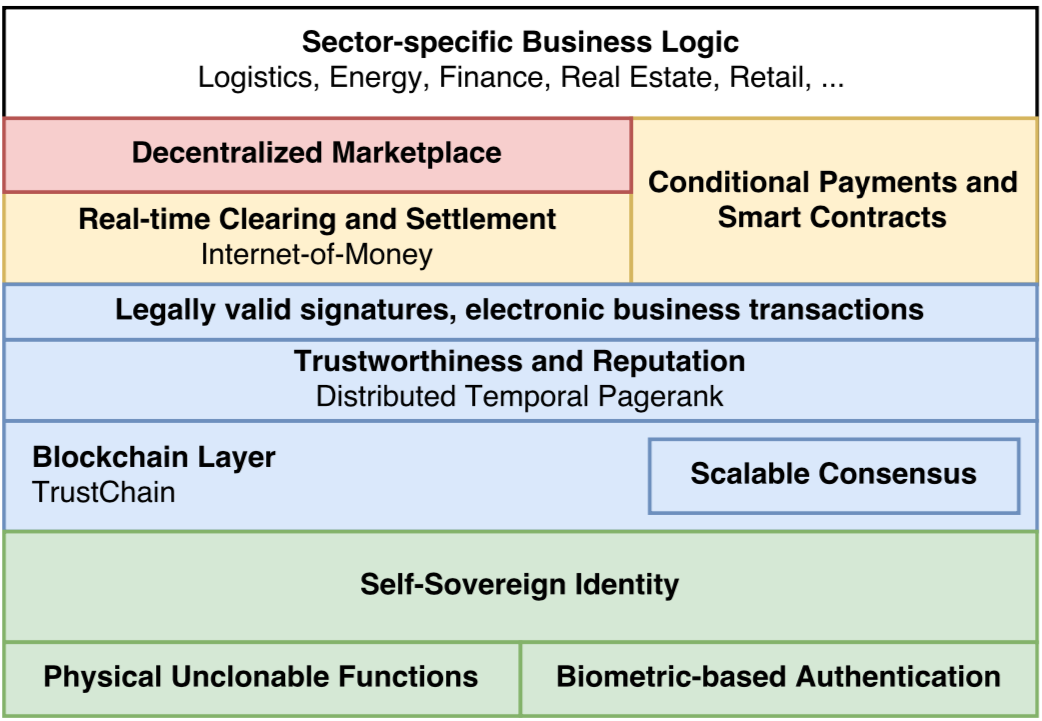
\includegraphics[width={0.8\textwidth}]{images/stack_ssi}}
    \caption{Detailed technology portfolio for trust creation in the blockchain age \cite{pouwelse}. As shown in the bottom of this figure, Physical Unclonable Functions and biometric-based authentication are utilized to secure the self-sovereign identity.}
    \label{fig:trust-creation}
\end{figure}

An example of PUF type is SRAM PUF. SRAM, stands for \textit{static random-access memory}, is a type of semiconductor memory that uses bistable latching circuitry (flip-flop) to store each bit. When a static RAM (SRAM) is turned on, the memory cells have undefined states \cite{tuyls_2010}. The initialized values on the memory cells are also random and unique to each SRAM. Based on these properties, SRAM is considered as a reasonable candidate for PUF. The value of these bits itself is determined by the SRAM cell which consists of two cross-coupled inverters along with two access transistors. This concept was first introduced by Guajardo and Holcomb in 2007 \cite{guajardo_kumar_schrijen_tuyls}. In order for SRAM to be used as a cryptographic security key, SRAM PUFs need to have certain characteristics such as the key generated by every SRAM should be reliable and unique. Reliable means the generated key should always be consistent, while unique refers to there should be no correlation between one device and another.
Unfortunately, SRAM PUF is also problematic since it contains noise in its bit value. To handle the noise, error correction code is usually utilized.

% \chapter{\chapterThree}
% \label{chp:3}
\section{Problem Statement}


Since introduced by Guajardo and Holcomb in 2007, there have been many innovations in SRAM PUF field. A simple patent search using patents.google.com with query 'sram; puf' results in 546 results \cite{google_patents}. The number of articles in \seqsplit{scholar.google.com} also exhibit a high occurrences, shown 2,120 articles (citations and patents are not included) \cite{google_scholar}.
Even though these facts indicate a promising future for this concept, one also should notice that current state-of-the-art in this field mostly consists of one-off prototypes or specific proprietary implementations.
To get an SRAM PUF product from the market, one has to order a specific request from a company. For example, Intrinsic-ID, one of the main leaders in SRAM PUF technology, has a software-based solution which able to generate unique keys and identities for nearly all microcontrollers without a need for security-dedicated silicon \cite{broadkey}. Even though this solution exists and seems easy to use, unfortunately, they don't say specifically how much will it cost to use this solution.
They also have another solution for SRAM PUF which is focused on hardware IP (and supporting software/firmware) to enable designers to implement PUFs within their design. This solution has a high possibility to obstruct a small company or a single user to use their solution since usually this type of product are intended to use with an expensive contract. Similar to the software-based solution they offer, they also don't put the explicit price to use this product. An example of a product that uses this solution is FPGA Microsemi Polarfire \cite{polarfire}.

The SRAM PUF field lacks an Arduino, Linux, or GCC type of open reference implementation. A quick lookup in Github shows that there's no extensive open source project related to SRAM PUF there. There are projects corresponding to PUF concepts, but most of them also only delve into a simulation.
The communities seem to haven't established a wide agreement on which approach yields the strongest security properties.

An additional issue that we would like to address is SRAM PUF's application. As mentioned in Chapter 1, the importance of securing key and user's data is getting higher, especially with the introduction of self-sovereign identity. There are already many SRAM PUF applications published, but sadly, there isn't any example working project that tries to integrate SRAM PUF in self-sovereign identity concept. Most PUF applications are designed for authentication \cite{Tuyls2007} \cite{delvaux} \cite{Suh:2007:PUF:1278480.1278484} \cite{10.1007/978-3-642-04474-8_22} \cite{10.1007/978-3-642-10838-9_22} \cite{10.1007/978-3-319-29078-2_5}
and generating cryptographic keys \cite{Suh:2007:PUF:1278480.1278484} \cite{10.1007/978-3-642-33027-8_18}.

Based on these facts, we believe the next challenge for this field is to discover a common approach. The field needs to move beyond isolated single-person projects and single-company approaches towards a mature and sharing ecosystem. The field SRAM PUF requires a single implementation which is continuously improved upon for many years to come and is supported by the majority of the academic and commercial parties.
Furthermore, we also try to initiate an attempt of integration between PUF and self-sovereign identity by providing a scheme to protect user's data and key. This project will be useful in the process of self-sovereign identity development.

To understand our intention in this thesis better, this thesis' problem statement is presented here. The problem statement of this thesis is:

\begin{adjustwidth}{1cm}{1cm}
		\textit{How to develop an open source secure data protection and key storage scheme using off-the-shelf SRAM component and software-based SRAM PUF technology?}
		% \textit{How to develop an open source secure data protection and key storage scheme using off-the-shelf SRAM component based on SRAM PUF technology?}
    % \textit{How to develop a secure software-only SRAM PUF-based data protection and key storage scheme using off-the-shelf SRAM while providing a mature and sharing ecosystem for continuous SRAM PUF development?}
\end{adjustwidth}

Derived from the problem statement, there are two goals defined in this thesis. The first goal is to devise a secure data protection and key storage scheme based on SRAM PUF technology. The data and the key protected by the scheme has to be safe even though the PUF device is lost. Moreover, the scheme should work using off-the-shelf SRAM. This sub-goal leads us to another question, can we build SRAM PUF using off-the-shelf SRAM? If it is possible, what characteristics need to be fulfilled by off-the-shelf SRAM to be eligible as a PUF candidate?
In addition, the constructed SRAM PUF has to work without any hardware design, or in other words, software-based construction. The data protection and key storage functions inside the scheme will be helpful in addressing the problem of self-sovereign identity and keeping the secret key.
The next goal is to create a sharing ecosystem for the evolution of our data protection and key storage scheme. The ecosystem should be easily accessed and understood to encourage the academics and commercial parties to use and develop the ecosystem together. The easiest step to achieve this goal is by making our thesis as an open source project.


\section{Contributions}
In our work, we strongly believe in open source idea and communities involvement when developing a system. Combined with the problems and potential of SRAM PUF mentioned before,
% and also driven by passions, willing to learn, and extensive brainstorming,
this thesis generates several additions into the state of the art of SRAM PUF knowledge. This thesis' contributions are explained below:
\begin{itemize}
    \item \textit{The first open source project on software-based SRAM PUF using off-the-shelf SRAM.}
    % This is the first open project on software-based SRAM PUF.
    % The project can be found on a Github repository \cite{repository}.
    This software-based SRAM PUF project consists of Arduino and Python codes and can be found on a Github repository \cite{repository}. It provides the off-the-shelf SRAM testing, enrollment and reconstruction mechanism which can be utilized to develop other applications. The testing part can be utilized to check whether an SRAM is capable to be a PUF root-of-trust or not. The enrollment stage will generate the helper data and the challenge which stored on a microSD connected to Arduino. The reconstruction part can generate a PUF-generated key based on the challenge and the helper data. In our construction, the selected off-the-shelf SRAM is Cypress CY62256NLL. We also tested another type of SRAM called Microchip 23LC1024 but we abandoned it due to insufficient results to be eligible as a PUF candidate. The enrollment stage also requires a bit selection algorithm called data remanence analysis. In the experiment part, there is another bit selection algorithm tested named neighbor analysis. This method is not selected due to worse performance than data remanence analysis.
    \item \textit{Procedure to develop an SRAM PUF-based application using any off-the-shelf SRAM.} The procedure consists of three main steps. First, one should test the off-the-shelf SRAM quality to be a PUF component. If passed, the procedure continues to the next step which consists of enrollment and reconstruction mechanism which will be able to create a PUF-generated key. Last, using the PUF-generated key, one can develop any PUF-based application.
    % Based on our SRAM PUF construction, we also come up with an idea on how to develop an SRAM PUF-based application
    \item \textit{A scheme to enable secure data and key storage using off-the-shelf SRAM and software-based SRAM PUF.} This scheme is influenced by multi-factor authentication. Using a combination of the PUF-generated key and user's password, a derived key is produced and utilized as the final key to protecting user's data or/and user's key.
    % \item \textit{An open ecosystem to develop SRAM PUF using off-the-shelf SRAM.} The ecosystem consists of source code (Arduino and python code) and recommendations on how to test a possible SRAM candidate that might be used as an SRAM PUF. Using the system, we present testing results of two off-the-shelf SRAMs; Microchip 23LC1024 and Cypress CY62256NLL. Both SRAMs are tested on voltage variation and time interval between enrollment testing. The system also provides a bit selection algorithm; data remanence. This algorithm is also tested on these two SRAMs along with another bit selection algorithm, neighbor stability analysis. Neighbor stability analysis is not included in the final version of the project due to worse performance compared to data remanence analysis.
    \item \textit{A concept to devise numerous CRPs using SRAM PUF.} One of SRAM PUF drawbacks is the limitation of possible challenge-response pairs. We propose to use a set of bit locations as the challenge since when using this concept, the number of possible pairs is the permutation of total bit locations over the required number of bit locations. The total possible CRPs using this concept is a significant large number which can be bigger than the total number of atom in earth.
    % \item \textit{A concept to devise a strong PUF using SRAM PUF.} Normally, SRAM PUF is considered a weak PUF due to the limitation of possible challenge-response pairs. We propose to use a set of bit locations as the challenge since when using this concept, the number of possible pairs is the permutation of total bit locations over the required number of bit locations. The total possible CRPs using this concept is a significant large number which may lead to a \textit{strong PUF} definition.
\end{itemize}


\section{Outline}
After explaining a brief review of SRAM's potentials and problems, problem statement and our contributions in this chapter,
Chapter \ref{chp:2} continues with an overview of security, cryptography, symmetric encryption, key derivation function and multi-factor authentication. Explanations of PUF and SRAM PUF are also presented in that chapter. Chapter \ref{chp:4} describes our proposed SRAM PUF development system, our idea on how to create numerous CRPs using SRAM PUF, and a scheme to enable secure data and key storage using SRAM PUF. Chapter \ref{chp:5} shows our implementation, experiments and results. Last chapter, Chapter \ref{chp:6}, summarizes this thesis and also gives our view on possible improvements on this project.


% % CHAPTERS ... For instance: History/Prior Work, Design/Implementation, Experiments
% \include{chapter_2}

\chapter{Introduction}

\textit{This chapter starts by presenting background and motivation on doing this thesis project. Afterwards, the problem statement and thesis' goals will be explained. Explanations on our contributions to the state-of-the-art will continue this chapter. This chapter will be closed by description of thesis' outline.}

\section{Need for Self-Sovereign Identity}
Hardly anyone can live without having their identity. Identity is the one that defines who we are, something which helps to describe the uniqueness of everyone.
Identity's role in our daily life is unquestionable. Society requires identity systems to enable identity-requiring transactions at scale, allowing procedures that require the formal asking and answering of identity queries in place, allowing millions of transactions to occur.
In modern society, identity is commonly related to social security cards, driver's licenses, and other state-issued credentials. Centralized controlled by the government is the definition of these elements.

Along with the rise of the digital age, identity also redefines itself. Identity in the digital world, can be referred as digital identity, is split into multiple domains. Our Facebook identity does not correlate directly to our Twitter identity or to most other domains. Digital identities are scattered, vary from one Internet domain to another. Scattered identities which locked to multiple entities leads to a problem where users are helpless in front of an authority who can deny their identity or even confirm a false identity. This phenomenon ignites a problem where users are not in control of their identity.
There is no clear construction and agreement on how to build the digital identity which usable across platforms. This is an unfortunate since lack of digital identity also limits the development and delivery of efficient, secure, digital-based economy and society \cite{blueprint}. The failure to solved the digital identity problem issue even looks a bit strange since we already have \textit{public key cryptography} since 1984, introduced by Chaum \cite{chaum}, which enable secure communication between parties without the hassle of key distribution problem and also provide valid digital signatures. Using public key cryptography, anyone who wants to send any message to a recipient needs to encrypt their message using the recipient's public key. Afterwards, the recipient can read the message after decrypting the received message using its private key.

To fix the scattered identity issue, a solution was proposed: one should be able to store their encrypted data in their own devices. To use the data, a service has to ask the data owner for the private key which will be used to decrypt the data. Using this concept, everyone has to keep their secret keys secure and solely in their possession.
A centralized storage of private keys is out of question since it will be a honeypot for cyber attacks. Simply put, keeping secret keys secure is the cardinal problem to solve here.


All problems mentioned before lead to a thinking: identity and secure key storage need to be solved in a decentralized manner.
In 2012, a new concept called \textit{self-sovereign identity} (SSI) arise \cite{moxytongue}.
Self-sovereign identity is a decentralized identity concept which capable of authenticating statements, without any central organization, point-of-failure or any possibility of data tracking \cite{pouwelse}. Self-sovereign identity will be able to give users full control over their identity. In simple words, users can store their identity data on their devices, and decide whether to give access to anyone who is willing to use it or not. In addition, there will be no need for a centralized storage since each user database is distributed among themselves. A high possibility to get this concept popular is also present with the introduction of the European Union General Data Protection Regulation \cite{eur-lex}.

At the end of 2017, Johan Pouwelse and Martijn de Vos proposed an SSI design which focused on data protection \cite{pouwelse}.
Data protection itself is related to securing data against unauthorized access \cite{data_protection_scheme}.
Their proposal is described by a concept where the user data are encrypted and never leave the device/domain. Any operation which requires the data, such as authentication, will require symmetric encryption on the encrypted data. This encrypted data should be securely protected and the domain should be trustworthy. In addition, the key used to encrypt and decrypt data should be kept securely.

The most common way to store the key is by using a \textit{non volatile memory} (NVM). NVM is a type of computer memory that keep intact its information without requiring a continuous power supply. An example of a product which uses NVM to store the key is a debit card where it uses its chip to store information. Unfortunately, this NVM is prone to physical attack. Since the key is permanently stored in the memory, an attacker can use some technique to clone the memory, such as \textit{microprobing} \cite{skorobogatov_2011}.  An attacker may also use a side channel information to retrieve any information about the key.
% There are numerous other techniques for physical attack.
This attack can be even worse if someone that knows the system design is involved. Due to this problem, more secure, tamper-evident, tamper-proof solutions need to be presented.

\section{Rise of PUF as a Security Solution}
\label{ris_puf}
In 2001, Physical Unclonable Function (PUF) comes in handy as an inexpensive and yet effective security solution to overcome the mentioned problem before by a different way of generating and processing secret keys in security hardware. It was introduced by Pappu \cite{Pappu2026}. Unlike cryptographic algorithm security which usually relies on a hard-to-solve mathematical problem, PUF idea stems from using hardware features designed to utilize the physical random nanoscale disarray phenomena \cite{retrospective}. These disarray phenomena can be used as a derivation of keys without having to keep any security-critical information explicitly. This physical randomness is unclonable, even by the original manufacturer due to manufacturing process variations. Furthermore, since the secrets can only be produced when the PUF device is turned on, active manipulation of circuit structure will cause dysfunction of challenge-response mechanism and destroy the secret.

Related to self-sovereign identity concept, \cite{pouwelse} present an idea to use PUF and biometric-based authentication to securely protect the data in the self-sovereign identity. Figure \ref{fig:trust-creation} shows the detailed technology stack in their trust creation proposal on how to build trust in the blockchain era.

\begin{figure}[tph!]
    \centerline{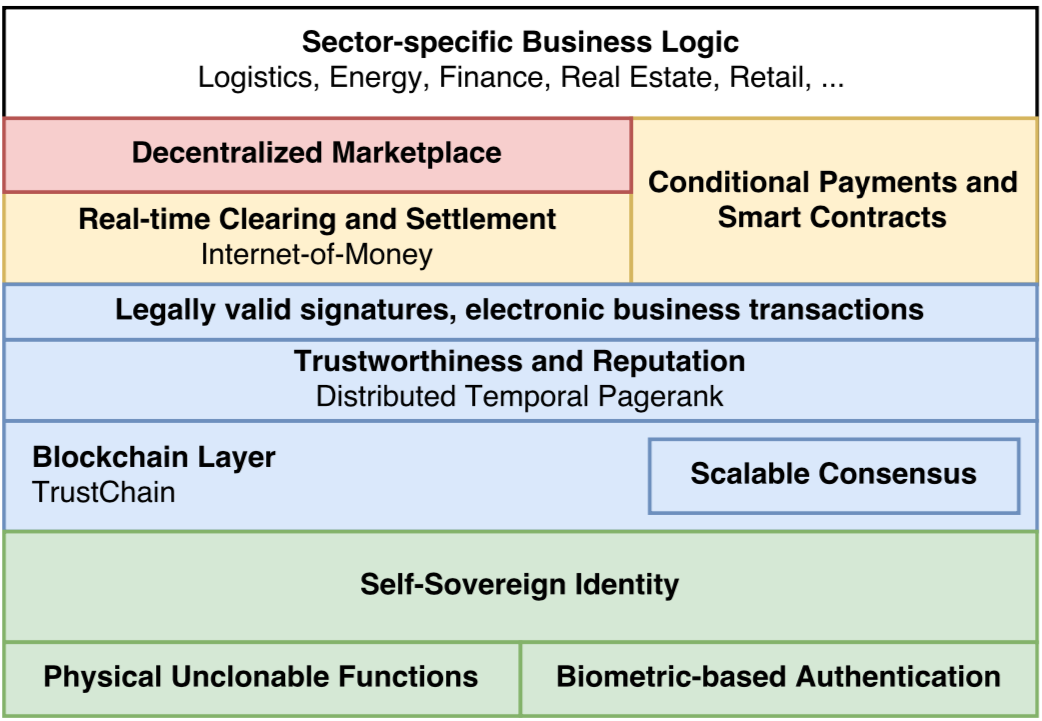
\includegraphics[width={0.8\textwidth}]{images/stack_ssi}}
    \caption{Detailed technology portfolio for trust creation in the blockchain age \cite{pouwelse}. As shown in the bottom of this figure, Physical Unclonable Functions and biometric-based authentication are utilized to secure the self-sovereign identity.}
    \label{fig:trust-creation}
\end{figure}

An example of PUF type is SRAM PUF. SRAM, stands for \textit{static random-access memory}, is a type of semiconductor memory that uses bistable latching circuitry (flip-flop) to store each bit. When a static RAM (SRAM) is turned on, the memory cells have undefined states \cite{tuyls_2010}. The initialized values on the memory cells are also random and unique to each SRAM. Based on these properties, SRAM is considered as a reasonable candidate for PUF. The value of these bits itself is determined by the SRAM cell which consists of two cross-coupled inverters along with two access transistors. This concept was first introduced by Guajardo and Holcomb in 2007 \cite{guajardo_kumar_schrijen_tuyls}. In order for SRAM to be used as a cryptographic security key, SRAM PUFs need to have certain characteristics such as the key generated by every SRAM should be reliable and unique. Reliable means the generated key should always be consistent, while unique refers to there should be no correlation between one device and another.
Unfortunately, SRAM PUF is also problematic since it contains noise in its bit value. To handle the noise, error correction code is usually utilized.

% \chapter{\chapterThree}
% \label{chp:3}
\section{Problem Statement}


Since introduced by Guajardo and Holcomb in 2007, there have been many innovations in SRAM PUF field. A simple patent search using patents.google.com with query 'sram; puf' results in 546 results \cite{google_patents}. The number of articles in \seqsplit{scholar.google.com} also exhibit a high occurrences, shown 2,120 articles (citations and patents are not included) \cite{google_scholar}.
Even though these facts indicate a promising future for this concept, one also should notice that current state-of-the-art in this field mostly consists of one-off prototypes or specific proprietary implementations.
To get an SRAM PUF product from the market, one has to order a specific request from a company. For example, Intrinsic-ID, one of the main leaders in SRAM PUF technology, has a software-based solution which able to generate unique keys and identities for nearly all microcontrollers without a need for security-dedicated silicon \cite{broadkey}. Even though this solution exists and seems easy to use, unfortunately, they don't say specifically how much will it cost to use this solution.
They also have another solution for SRAM PUF which is focused on hardware IP (and supporting software/firmware) to enable designers to implement PUFs within their design. This solution has a high possibility to obstruct a small company or a single user to use their solution since usually this type of product are intended to use with an expensive contract. Similar to the software-based solution they offer, they also don't put the explicit price to use this product. An example of a product that uses this solution is FPGA Microsemi Polarfire \cite{polarfire}.

The SRAM PUF field lacks an Arduino, Linux, or GCC type of open reference implementation. A quick lookup in Github shows that there's no extensive open source project related to SRAM PUF there. There are projects corresponding to PUF concepts, but most of them also only delve into a simulation.
The communities seem to haven't established a wide agreement on which approach yields the strongest security properties.

An additional issue that we would like to address is SRAM PUF's application. As mentioned in Chapter 1, the importance of securing key and user's data is getting higher, especially with the introduction of self-sovereign identity. There are already many SRAM PUF applications published, but sadly, there isn't any example working project that tries to integrate SRAM PUF in self-sovereign identity concept. Most PUF applications are designed for authentication \cite{Tuyls2007} \cite{delvaux} \cite{Suh:2007:PUF:1278480.1278484} \cite{10.1007/978-3-642-04474-8_22} \cite{10.1007/978-3-642-10838-9_22} \cite{10.1007/978-3-319-29078-2_5}
and generating cryptographic keys \cite{Suh:2007:PUF:1278480.1278484} \cite{10.1007/978-3-642-33027-8_18}.

Based on these facts, we believe the next challenge for this field is to discover a common approach. The field needs to move beyond isolated single-person projects and single-company approaches towards a mature and sharing ecosystem. The field SRAM PUF requires a single implementation which is continuously improved upon for many years to come and is supported by the majority of the academic and commercial parties.
Furthermore, we also try to initiate an attempt of integration between PUF and self-sovereign identity by providing a scheme to protect user's data and key. This project will be useful in the process of self-sovereign identity development.

To understand our intention in this thesis better, this thesis' problem statement is presented here. The problem statement of this thesis is:

\begin{adjustwidth}{1cm}{1cm}
		\textit{How to develop an open source secure data protection and key storage scheme using off-the-shelf SRAM component and software-based SRAM PUF technology?}
		% \textit{How to develop an open source secure data protection and key storage scheme using off-the-shelf SRAM component based on SRAM PUF technology?}
    % \textit{How to develop a secure software-only SRAM PUF-based data protection and key storage scheme using off-the-shelf SRAM while providing a mature and sharing ecosystem for continuous SRAM PUF development?}
\end{adjustwidth}

Derived from the problem statement, there are two goals defined in this thesis. The first goal is to devise a secure data protection and key storage scheme based on SRAM PUF technology. The data and the key protected by the scheme has to be safe even though the PUF device is lost. Moreover, the scheme should work using off-the-shelf SRAM. This sub-goal leads us to another question, can we build SRAM PUF using off-the-shelf SRAM? If it is possible, what characteristics need to be fulfilled by off-the-shelf SRAM to be eligible as a PUF candidate?
In addition, the constructed SRAM PUF has to work without any hardware design, or in other words, software-based construction. The data protection and key storage functions inside the scheme will be helpful in addressing the problem of self-sovereign identity and keeping the secret key.
The next goal is to create a sharing ecosystem for the evolution of our data protection and key storage scheme. The ecosystem should be easily accessed and understood to encourage the academics and commercial parties to use and develop the ecosystem together. The easiest step to achieve this goal is by making our thesis as an open source project.


\section{Contributions}
In our work, we strongly believe in open source idea and communities involvement when developing a system. Combined with the problems and potential of SRAM PUF mentioned before,
% and also driven by passions, willing to learn, and extensive brainstorming,
this thesis generates several additions into the state of the art of SRAM PUF knowledge. This thesis' contributions are explained below:
\begin{itemize}
    \item \textit{The first open source project on software-based SRAM PUF using off-the-shelf SRAM.}
    % This is the first open project on software-based SRAM PUF.
    % The project can be found on a Github repository \cite{repository}.
    This software-based SRAM PUF project consists of Arduino and Python codes and can be found on a Github repository \cite{repository}. It provides the off-the-shelf SRAM testing, enrollment and reconstruction mechanism which can be utilized to develop other applications. The testing part can be utilized to check whether an SRAM is capable to be a PUF root-of-trust or not. The enrollment stage will generate the helper data and the challenge which stored on a microSD connected to Arduino. The reconstruction part can generate a PUF-generated key based on the challenge and the helper data. In our construction, the selected off-the-shelf SRAM is Cypress CY62256NLL. We also tested another type of SRAM called Microchip 23LC1024 but we abandoned it due to insufficient results to be eligible as a PUF candidate. The enrollment stage also requires a bit selection algorithm called data remanence analysis. In the experiment part, there is another bit selection algorithm tested named neighbor analysis. This method is not selected due to worse performance than data remanence analysis.
    \item \textit{Procedure to develop an SRAM PUF-based application using any off-the-shelf SRAM.} The procedure consists of three main steps. First, one should test the off-the-shelf SRAM quality to be a PUF component. If passed, the procedure continues to the next step which consists of enrollment and reconstruction mechanism which will be able to create a PUF-generated key. Last, using the PUF-generated key, one can develop any PUF-based application.
    % Based on our SRAM PUF construction, we also come up with an idea on how to develop an SRAM PUF-based application
    \item \textit{A scheme to enable secure data and key storage using off-the-shelf SRAM and software-based SRAM PUF.} This scheme is influenced by multi-factor authentication. Using a combination of the PUF-generated key and user's password, a derived key is produced and utilized as the final key to protecting user's data or/and user's key.
    % \item \textit{An open ecosystem to develop SRAM PUF using off-the-shelf SRAM.} The ecosystem consists of source code (Arduino and python code) and recommendations on how to test a possible SRAM candidate that might be used as an SRAM PUF. Using the system, we present testing results of two off-the-shelf SRAMs; Microchip 23LC1024 and Cypress CY62256NLL. Both SRAMs are tested on voltage variation and time interval between enrollment testing. The system also provides a bit selection algorithm; data remanence. This algorithm is also tested on these two SRAMs along with another bit selection algorithm, neighbor stability analysis. Neighbor stability analysis is not included in the final version of the project due to worse performance compared to data remanence analysis.
    \item \textit{A concept to devise numerous CRPs using SRAM PUF.} One of SRAM PUF drawbacks is the limitation of possible challenge-response pairs. We propose to use a set of bit locations as the challenge since when using this concept, the number of possible pairs is the permutation of total bit locations over the required number of bit locations. The total possible CRPs using this concept is a significant large number which can be bigger than the total number of atom in earth.
    % \item \textit{A concept to devise a strong PUF using SRAM PUF.} Normally, SRAM PUF is considered a weak PUF due to the limitation of possible challenge-response pairs. We propose to use a set of bit locations as the challenge since when using this concept, the number of possible pairs is the permutation of total bit locations over the required number of bit locations. The total possible CRPs using this concept is a significant large number which may lead to a \textit{strong PUF} definition.
\end{itemize}


\section{Outline}
After explaining a brief review of SRAM's potentials and problems, problem statement and our contributions in this chapter,
Chapter \ref{chp:2} continues with an overview of security, cryptography, symmetric encryption, key derivation function and multi-factor authentication. Explanations of PUF and SRAM PUF are also presented in that chapter. Chapter \ref{chp:4} describes our proposed SRAM PUF development system, our idea on how to create numerous CRPs using SRAM PUF, and a scheme to enable secure data and key storage using SRAM PUF. Chapter \ref{chp:5} shows our implementation, experiments and results. Last chapter, Chapter \ref{chp:6}, summarizes this thesis and also gives our view on possible improvements on this project.

% \chapter{Introduction to Security}

\section{Secure System Necessity}
How valuable is our data? How much would company for accessing those information? These questions might be silly but if we consider that there are many companies which thrived using our data (e.g. Facebook, Twitter, and Uber), we should reconsider how much should we value our data. I know these data if we value each element might not worth much, most will worth significant when these data is combined together to bring a more insight information. But what about the sensitive data which its value can worth millions of dollars, such as the bitcoin key? In \cite{bitcoin}, the highest bitcoin address is worth 1.4B US\$ and there are 513,562 addresses which has value more than 10000 US\$. Due to their high values, these data, the key to these addresses, must be protected.

Before going further, we should understand first what kind of attacks possibly affecting these data. Similar like in the physical world, in the digital world, adversaries' intention can be either mischievious, non-malicious or accidental. Some example of mischievious activities are stealing information and modifying the data. Accidental can happen due to human error. These three types of adversaries' intention can lead to a significant number of attacks and threats.

Now, two questions are arised. Is there are a way that guarantee 100\% of these data protection? Is there any bullet-proof secure system? Unfortunately, there is no such thing as a 100\% secure system. Fortunately, there are ways to design a system to be as secure as possible in a limited scope, usually defined as secure 'from who' and 'from what'. According to \cite{Pfleeger}, computer security is "the protection of the items you value, called the assets of a computer or a computer system." In the scope of data mentioned before, the assets are the bitcoin keys and addresses.

To help defining a secure system, common security requirements are mentioned.
According to \cite{cryptography_decrypted}, there are four elements on common security, which are:
\begin{itemize}
  \item \textit{Confidentiality}: a piece of information should be accesible only to an authorized users. For example, an encrypted data can only be decrypted by the secret key owner.
  \item \textit{Authentication}: assurance of the sender of a message, date of origin, data content, time sent, data information, etc. are correctly identified.
  \item \textit{Integrity}: any assets can only be modified by an authorized subjects. For example, data should be keep intact during transmission
  \item \textit{Non-repudiation}: a subject should be prevented from denying previous actions. For example, a sender cannot deny the data which it sent.
\end{itemize}

\section{Cryptography}
One way to achieve these four security requirements is by using cryptography. In traditional definition, cryptography can be defined as the art of writing or solving codes \cite{Oxford_dictionary}. But this definition is inaccurate to use nowadays because instead of depending on creativity and personal skill when constructing or breaking codes, the modern cryptography focus their definition using science and mathematics. According to \cite{modern_cryptography}, modern cryptography can be defined as "the scientific study of techniques for securing digital information, transactions, and distributed computations." The algorithm which use cryptography as their main point is called cryptographic algorithm.

Since the birth of cryptography, its main concerned is usually related on securing communication which can be achieved by constructing \textit{ciphers} to provide secret communication between parties involved. The construction of ciphers to ensure only authorized parties also can be called as encryption schemes.
There are two types of cryptographic algorithm, symmetric and asymmetric algorithm. Symmetric, also known as private key encryption or private key cryptography, requires the same key for encryption and decryption. Meanwhile in asymmetric algorithm (can be referred as public key encryption or public key cryptography), there are two keys utilized; private key and public key. Public key is utilized for encryption and private key is used for decryption. One of the main advantage of symmetric encryption over asymmetric encryption is it requires less computational power which make it suitable to use in embedded devices.
Further explanation on symmetric encryption algorithm will be provided in the next chapter.

% \input{chapter/chapter3}
% \chapter{Background Theory}
\chapter{\chapterTwo}
\label{chp:2}

\textit{This chapter examines some background theory related to security, cryptography, and PUF. A brief review of security is presented, followed by explanations on symmetric cryptography, key derivation function and multi-factor authentication.
Then, theories related to PUF and SRAM PUF are described, continued by evaluation on some PUF-based applications. We also present previous publications which related to SRAM PUF built using off-the-shelf SRAM.}

\section{Security Requirements and Cryptography}
\label{chapter2.1}

A perfect and 100\% secure system is the holy grail of all computing system. Unfortunately, such thing does not exist. The best way to achieve that goal is by designing a system to be as secure as possible in a limited scope.
To help defining a secure system, common security requirements are mentioned.
According to \cite{cryptography_decrypted}, there are four elements on common security, which are:
\begin{itemize}
  \item \textit{Confidentiality}: a piece of information should be accessible only to an authorized user. For example, an encrypted data can only be decrypted by the secret key owner.
  \item \textit{Authentication}: assurance of the sender of a message, date of origin, data content, time sent, data information, etc. are correctly identified.
  \item \textit{Integrity}: any assets can only be modified by authorized subjects. For example, data should be kept intact during transmission.
  \item \textit{Non-repudiation}: a subject should be prevented from denying previous actions. For example, a sender cannot deny the data which it sent.
\end{itemize}

One way to achieve these four security requirements is by using cryptography. In traditional definition, cryptography can be defined as the art of writing or solving codes \cite{Oxford_dictionary}. But this definition is inaccurate to use nowadays because instead of depending on creativity and personal skill when constructing or breaking codes, the modern cryptography focuses their definition using science and mathematics. According to \cite{modern_cryptography}, modern cryptography can be defined as "the scientific study of techniques for securing digital information, transactions, and distributed computations." The algorithm which uses cryptography as their main point is called cryptographic algorithm.

Since the birth of cryptography, its main concerned is usually related to securing communication which can be achieved by constructing \textit{ciphers} to provide secret communication between parties involved. The construction of ciphers to ensure only authorized parties also can be called as encryption schemes.
There are two types of cryptographic algorithm; symmetric and asymmetric algorithm. Symmetric, also known as private key encryption or private key cryptography, requires the same key for encryption and decryption. Meanwhile, in the asymmetric algorithm (can be referred as public key encryption or public key cryptography), there are two keys utilized; private key and public key. A public key is utilized for encryption and a private key is used for decryption. One of the main advantages of symmetric encryption over asymmetric encryption is it requires less computational power which makes it suitable to use in embedded devices.

\section{Symmetric Encryption}

According to \cite{modern_cryptography}, symmetric encryption consists of three algorithms which are:
\begin{itemize}
    \item \large{\textit{Gen}}: key-generation algorithm
    \item \large{\textit{Enc}}: encryption algorithm
    \item \large{\textit{Dec}}: decryption algorithm
\end{itemize}
To illustrate this better, an example using two parties, Alice and Bob are given. Before using the encryption or decryption algorithm, both parties will agree on a shared secret key $k$. This phase can be referred as \large{Gen}.
Afterwards, Alice can use the encryption algorithm (\large{Enc}) $E_k$ using the shared secret key $k$ on a message $m$ which will generates a ciphertext $c$. This procedure can be noted as $c\ =\ E_k(m)$. Bob can read the message by using the decryption algorithm (\large(Dec)) $Dec_k$ using the same shared secret key $k$. Decryption will result in the plaintext message $m$. This can be noted as $m\ =\ D_k(c)$.


There are many examples of symmetric encryption algorithms, such as RC2, DES, 3DES, RC6, Blowfish, and AES. AES algorithm will be explained below.

\subsubsection{AES}
AES, stands for Advanced Encryption Standard, is an encryption algorithm based on a substitution-permutation network and established by the U.S. National Institute of Standards and Technology (NIST) in 2001.
The block size inside AES has a size of 128 bits, while the key size can be either 128, 192, or 256 bits. The key size  itself describes the number of rounds which convert the plaintext into the ciphertext. If 128-bit key is used, there are 10 rounds utilized. 192-bit key leads to 12 rounds, while 14 rounds is used when 256-bit key is applied.


There are four major parts inside AES; \textit{KeyExpansions}, \textit{InitialRound}, \textit{Rounds} and \textit{FinalRound}. In KeyExpansions, the round keys are generated using Rijndael's key schedule
 based on the AES key.
Inside a normal round, there are four stages required to do; \textit{SubBytes}, \textit{ShiftRows}, \textit{MixColumns}, and \textit{AddRoundKey}.
SubBytes refers to a non-linear substitution procedure using a lookup table. ShiftRows means an act of shifting cyclically the last three rows of the state. MixColumns contains a mixing activity on the columns of the state.
AddRoundKey involves a fusing process of each byte of the state with a block of the round key utilizing bitwise xor operation. The difference between InitialRound, Rounds, and FinalRound is InitialRound only contain AddRoundKey, FinalRound does not has MixColumns inside, and Rounds just filled with those four stages.

An encryption can be done by following all these four parts. To convert ciphertext into the original plaintext, it is only required to apply a set of reverse rounds using the same encryption key.

\section{Key Derivation Function}
Besides the encryption algorithm, a \textit{key derivation function} (KDF) is one of the most utilized components of cryptographic applications. Its importance is due to its ability to convert a stable secret, usually contain sufficient amount of randomness but non-uniformly distributed,  $Z$ into one or more cryptographically strong secret keys $k\ \epsilon\ {0,1}^K$.
Cryptographically strong itself refers to indistinguishability by reasonable computation from a random uniform string with similar length \cite{key_derivation}.
KDF can also be referred as a strong extractor.

A popular example of KDF is a keyed cryptographic hash function (can be referred as \textit{HMAC}, stands for hash-based message authentication code).
% The difference between keyed cryptographic hash function and a normal hash function is a keyed hash function requires an additional \textit{salt} as an input (besides the key to derived).
The formula for HMAC is shown below \cite{rfc2104}:
\begin{equation}
  {\displaystyle \operatorname {HMAC} (K,m)=H{\Bigl (}(K'\oplus opad)\|H{\bigl (}(K'\oplus ipad)\|m{\bigr )}{\Bigr )}}
\end{equation}
There are three elements which defined the cryptographic strength of the HMAC; the utilized hash function's cryptographic strength, the output size, and the key's size and quality. Currently, the latest cryptographic hash function standard published by the National Institute of Standards and Technology (NIST) as a U.S. Federal Information Processing Standard (FIPS) is SHA-3 (introduced in 2015). SHA-3 (Secure Hash Algorithm 3) is a part of another cryptographic primitive family called Keccak \cite{10.1007/978-3-642-38348-9_19}. Keccak is built on top of an method called sponge construction. Sponge construction itself is based on multiple layers of pseurandom function where each layer is able of absorbing (receiving input) and squeezing (generating output) any amount of data.

There are three requirements need to be fulfilled as a secure cryptographic hash function; \textit{preimage resistant, second preimage resistant, and collision resistant}. Preimage resistant means it should be hard to find a message with a given hash value. In second preimage resistant, if one message is provided, it should be hard to find another message with the same hash value.
Last, collision resistant refers to difficultness to find two messages with the same hash value. HMAC built using SHA-3 with key length of 256 bits has collision resistance of 128 bits, preimage resistance of 256 bits, and second preimage resistant of	256 bits \cite{technology2015sha}.

\section{Multi-factor Authentication}
\label{chp:2.mfa}
As mentioned in Section \ref{chapter2.1}, authentication refers to assuring any piece of information is correctly identified. Authentication can be done using any of these elements/factors; knowledge (a piece of information which only known by the user, e.g. password), possession (any object which only owned by the user, e.g. RFID card), or inherence (something which uniquely describe the user, e.g. fingerprint). If two or more elements are combined together for authentication, this leads to \textit{multi-factor authentication}. To understand the security level among all possible combinations, Figure \ref{fig:authentication} is provided. The highest possible security level is when these three factors are combined together.

\begin{figure}[tph!]
    \centerline{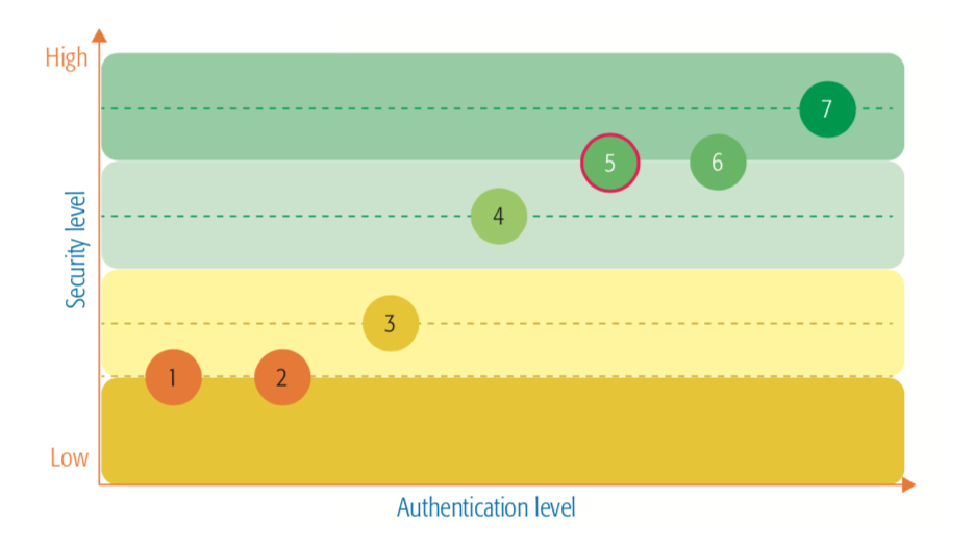
\includegraphics[width={0.5\textwidth}]{images/authentication}}
    \caption{Authentication systems security levels: (1) knowledge; (2) possession; (3) knowledge + inherence; (4) inherence; (5) possession + inherence; (6) knowledge + inherence; (7) knowledge + possesion + inherence \cite{Galdi2018ExploringNA}.}
    \label{fig:authentication}
\end{figure}


\section{Physically Unclonable Function}
A physically unclonable function (PUF) is an entity that utilizes manufacturing variability to produce a device-specific output. The idea to build PUF arise from the fact that even though the mask and manufacturing process is the same among different ICs, each IC is actually slightly different due to normal manufacturing variability \cite{retrospective}. PUFs leverage this variability to derive secret information that is unique to the chip. This secret can be referred as a silicon biometric.
In addition, due to the manufacturing variability that defines the secret, one cannot manufacture two identical chips, even with full knowledge of the chip’s design. PUF architectures exploit manufacturing variability in multiple ways. For example, one can utilize the effect of gate delay, the power-on state of SRAM, threshold voltages, and many other physical characteristics to derive the secret.

Due to this feature, PUFs are a promising innovative primitive that is used for authentication and secret key storage without the requirement of secure hardware. Currently, the best practice for providing a secure memory or authentication source in such a mobile system is to place a secret key in a nonvolatile electrically erasable programmable read-only memory (EEPROM) or battery-backed static random-access memory (SRAM) and use hardware cryptographic operations such as digital signatures or encryption.

There are two main parts of PUF, physical part, and operational part. Physical part refers to a physical system that is very difficult to clone due to uncontrollable process variations during manufacturing. Operational part means a set of \textit{challenges} (PUF input) $C_i$ has to be available to which the system responds with a set of sufficiently different \textit{responses} (PUF output) $R_i$. This combination of challenge and response is called \textit{challenge-response-pair} (CRP).
\begin{equation}
R_i <- PUF(C_i)
\end{equation}

The common application on using PUF usually requires two phases; the first phase is called \textit{enrollment} and the second one is usually referred as \textit{validation}. In enrollment, a number of CRPs are gathered from a PUF and then stored. In validation phase, a challenge from the stored CRPs is given to the PUF. Afterwards, the PUF response from this challenge is compared with the corresponding response from the database. The response is considered to be valid if there's a CRP from the stored CRPs related to this challenge and response. The validation phase can also be referred as \textit{reconstruction} phase since this phase involves a reconstruction of a response given a challenge.

According to \cite{retrospective}, to be qualified as PUF, a device should fulfill several characteristics below :
\begin{itemize}
\item \textit{Reliable}: A response to the same challenge should be able to be reproduced over time and over a various range of conditions.
\item \textit{Unpredictable}: A response to a challenge on a PUF device should be unrelated to a response to another challenge from the same device or the same challenge from a different device.
\item \textit{Unclonable}: Challenge-response pairs mapping of a device should be unique and cannot be duplicated.
\item \textit{Physically Unbreakable}: Any physical attempts to maliciously modify the device will result in malfunction or permanent damage.
\end{itemize}

\subsection{PUFs Classification} \label{lbl:puf-classification}

In this subsection, two subtypes of PUFs so-called "Weak PUFs" and "Strong PUFs" are presented.  The explanations on both types can be found below \cite{6800561}:
\begin{itemize}
\item Strong PUFs\newline
Strong PUFs can be recognized by possessing a tremendous number of CRPs which prevent an adversary to read all possible CRPs even if he has open access to the challenge-response interface. Anyone can freely give any challenge and read the response without affecting its security. In addition, even if he has a large subset of CRPs, he still cannot predict another yet unknown CRPs. Strong PUFs typically used for authentication.
\item Weak PUFs\newline
Weak PUFs can be identified by having few CRPs. Unlike the strong PUFs, weak PUFs require an access-restricted to the challenge-response mechanism. This means that even if an adversary holds a possession of the PUF device, he cannot read the response from a challenge or give any challenge to the PUF device. Weak PUFs commonly used for key storage and key generation.
\end{itemize}

Besides the number of CRPs, PUFs can also be categorized based on their physical design. There are two major categories, extrinsic and intrinsic PUFs \cite{maes_2016}.

Extrinsic means that it needs extra hardware added to the PUF component. The extra hardware is required to access the PUF component. There are two subcategories of extrinsic PUFs, non-electronic and analog electronic PUFs. Some examples in non-electronic PUFs are optical PUF, paper PUF, CD PUF, RF-DNA PUF, magnetic PUF, and acoustic PUF. Some design instances in analog electronic PUFs are VT PUF, power distribution PUF, coating PUF, and LC PUF.

In intrinsic, the PUF component has to be available naturally during the manufacturing process. In addition, PUF and the measurement equipment should be fully integrated with intrinsic PUF. There are two subcategories in intrinsic PUFs, delay based and memory based PUFs. An example of delay based PUF is arbiter PUF. The main principle of arbiter PUF is by presenting a race condition on two different routes on a chip where the winner will be decided by an arbiter circuit \cite{study_of_the_art_puf}. As in memory based PUFs, some examples of this design are SRAM PUF, butterfly PUF and latch PUF. SRAM PUF utilized the random physical mismatch in the cell introduced by manufacturing variability which controls the power-up behavior (can be zero, one, or no preference) \cite{study_of_the_art_puf}. Butterfly PUF use the effect of cross coupling between two transparent data latches. Using the functionalities of the latches, an unsteady condition can be initiated after which the circuit resolves back to one of the two stable states \cite{study_of_the_art_puf}. In latch PUF, the concept is based on using two NOR gates which are cross-coupled. These gates will lead to a stable condition depending on the internal discrepancy between the electronic components.

\subsection{Hamming Distances as an Identification Helper}

As explained before, PUF main purpose is dedicated for identification, shown by having a device-specific output. In PUF, \textit{hamming distance} is commonly used as a way to help defining this idea. Hamming distance itself is the number of positions at which the corresponding symbols are different on two equal length strings \cite{hamming_distance}.
There are two types of hamming distance utilized, intra-chip and inter-chip hamming distance. Inter-chip hamming distance is the distance between two responses resulting from giving a similar challenge to two distinct PUF devices \cite{study_of_the_art_puf}. Intra-chip hamming distance refers to the difference between the two responses resulting from applying a challenge twice to a PUF device \cite{modeling_sram}. To ease the identification purpose, fractional hamming distance is also introduced. Fractional hamming distance is the number of differences between two strings divided by the length of the bit strings.
In ideal PUFs, the intra-chip fractional hamming distance (HD\textsubscript{intra}) is 0\% and inter-chip fractional hamming distance (HD\textsubscript{inter}) is 50\%. Due to noises, normally PUF devices has HD\textsubscript{intra} $\leq$ 10\% and HD\textsubscript{inter} ~50\%. The identification goal will not be achieved if there is an overlap between HD\textsubscript{intra} and HD\textsubscript{inter} \cite{impact_aging}. Overlap will happen if the HD\textsubscript{intra} is too large and HD\textsubscript{inter} is too small, e.g. HD\textsubscript{intra} is 35\% and HD\textsubscript{inter} is 30\%.

\subsection{Helper Data Algorithms and Fuzzy Extractor}

There are two issues if PUF raw responses are used as a key in cryptographic primitive. First, both weak and strong PUFs rely on analog physical properties of the fabricated circuit to derive secret information. Naturally, these analog properties have noise and variability associated with them.
This can be a problem due to sensitivity of cryptographic functions on noises of their inputs.
Another issue is the PUF raw responses usually are not uniformly distributed, which makes it unqualified as a cryptographically secure key. These two issues can be solved using \textit{Helper Data Algorithm} (HDA). One can also refer Helper Data Algorithm as \textit{fuzzy extractor} since both are capable of converting noisy information into keys usable for any cryptographic application \cite{efficient_helper} \cite{fuzzy_extractor}.

Fuzzy extractor solves both issues mentioned above by using two phases, \textit{information reconciliation} and \textit{privacy amplification}. In information reconciliation phase, possible bit errors are corrected to form a robust bit string \cite{soft_decision}. Information reconciliation is tightly related to error correction. In fact, a procedure to do information reconciliation based on error-correcting codes is called code-offset technique \cite{fuzzy_extractor}. Using code-offset technique, one should be able to reconstruct a bit string \textit{w} from a noisy version \textit{w'} as long as the Hamming distance between \textit{w} and \textit{w'} is limited to \textit{t}.
The second phase, privacy amplification, is a process to evolve this robust bit string into a full entropy key. Privacy amplification, also can be called as randomness extraction \cite{information_reconciliation}, can be done by utilizing two-way hash function.

Beside these two phases, fuzzy extractor also consists of two procedures, \large{Gen} and \large{Rep}. \large{Gen}, stands for \textit{generation}, is a probabilistic procedure which outputs an "extracted" string / key (secret) $R$ and a string (public) \textit{helper data} $P$ on input fuzzy data $w$. \large{Rep}, stands for \textit{reproduction}, is a deterministic function capable of recovering secret key $R$ from the string \textit{helper data} $P$ and any vector $w'$ as long as the Hamming distance between \textit{w}and \textit{w'} is limited to \textit{t}.
In \cite{stable_key_generation}, Taniguchi et. al illustrated the generation and reproduction procedure of fuzzy extractor on PUF which is shown in Figure \ref{fig:scheme-key-generator}.

\begin{figure}[tph!]
    \centerline{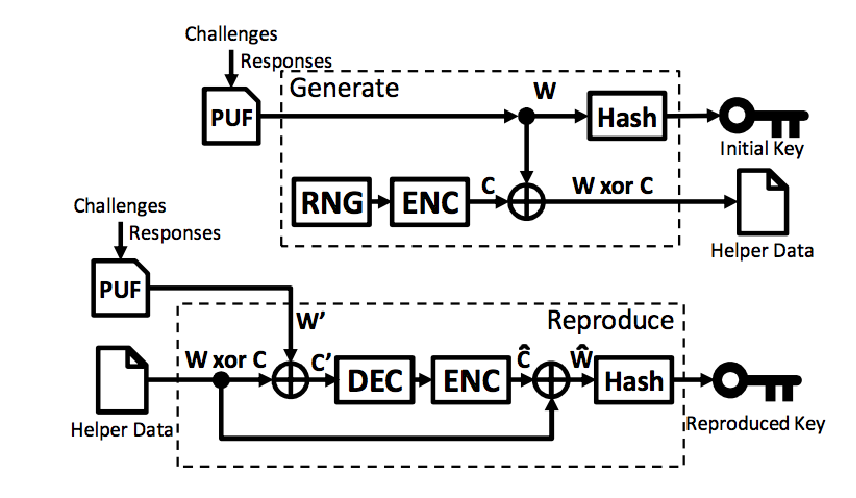
\includegraphics[width={0.8\textwidth}]{images/scheme_stable_key_generation}}
    \caption{Two procedures inside fuzzy extractor; generation and reproduction \cite{stable_key_generation}.}
    \label{fig:scheme-key-generator}
\end{figure}

\subsection{Error Correcting Codes}
To handle noises occurred inside a PUF, error-correcting codes (ECC) is employed.
Error-correcting codes are a class of schemes for encoding messages in an attempt to enable message recovery when there is noise introduced in the sending or receiving of the message. ECC can be divided into two subcategories, hard-decision and soft-decision. Hard-decision works on a predetermined set of values (usually 0 or 1 in a binary code), while a soft-decision decoder may take inputs on a span of values in-between (usually refers to float value).

There are some well-known ECC, such as in hard-decision code, Reed-Solomon code and BCH code; while in soft-decision, Viterbi code and turbo code. Soft-decision code has an advantage over hard-decision code where it can process extra information which indicates the reliability of each input data point and used to form better estimates of the original data. But it has drawback where one should provide a probability function on the data (on SRAM, a probability function on each cell should be provided) to enable a good decoding result.
% This is a problem if applied on this thesis goal where the system should work on any SRAM off-the-market. Calculating the probability on each SRAM cell will take an extra step, overcomplicate the system and the procedure on using the constructed system. Thus, the hard-decision code is preferred.

One of the popular hard-decision error correcting code is BCH codes. BCH, stands for \textit{Bose}–\textit{Chaudhuri}–\textit{Hocquenghem}, codes are a family of cyclic error correcting codes which constructed using polynomials over a finite field and work in a binary field.
BCH codes are a very flexible set of codes in that within certain bounds there is a great amount of choice in code parameters and are relatively efficient in message length and error correction. The code parameters are as follows:
\begin{itemize}
\item $q$: The number of symbols used (e.g., in binary field, $q = 2$)
\item $m$: The power to which to raise $q$ to generate a Galois Field for the construction of the code.
\item $d$: The minimum Hamming distance between distinct codewords.
\end{itemize}

These parameters lead to several derived parameters which are standard parameters of linear codes:
\begin{itemize}
\item $n$: The block length of the code; for our special case, $n = q*m \minus 1$
\item $t$: The number of errors that can be corrected, $d \geq 2t + 1$
\item $k$: The number of message bits in a codeword, $k \geq n - mt$
\end{itemize}

Both BCH codes and Reed-Solomon codes have the capability to correct multiple errors. Reed-Solomon codes are also a flexible ECC and have similar parameters as BCH codes, e.g. $n$, $k$, $d$.  Unlike BCH codes, Reed-Solomon codes can work in both binary and non-binary fields. Reed-Solomon codes also perform better in correcting burst errors while BCH codes are better at fixing random errors. BCH codes have an advantage where it requires less computing resource when working on the same parameter compared to Reed-Solomon codes.

\section{SRAM PUF}

SRAM PUF was first proposed by Guajardo and Holcomb in 2007. SRAM PUF uses existing SRAM blocks to generate chip-specific data.
Normally, when using SRAM to store data, a positive feedback is given to force the cell into one of the two states (a '1' or a '0') available. Once it is there, the cell will be stable and prevented from transitioning out of this state accidentally.

SRAM can be used as a PUF by utilizing its start-up values.
After powering-up the circuit, each cell stabilizes at a state which is defined by the mismatches between the involved transistors and provides one bit of output data. Since this mismatch determines the value of the power-up state of an SRAM cell, the power-up state of a cell will be biased towards 0 or 1 depends on the mismatch value. Since all SRAM cells have been affected by random process mismatches and non-identical, these start-up SRAM values can be utilized to generate a unique fingerprint \cite{dargar_2011}.

\subsection{Requirements for SRAM to be a PUF Component}\label{ch:requirement_sram_puf}
To be eligible as a PUF component, an SRAM has to have stable outputs which means any noise has to have little effect on its start-up behavior (shown by the value of HD\textsubscript{intra}). In addition, the distribution of 1's and 0's in the SRAM values ideally has to be equal (around 50:50) to ensure there is sufficient amount of randomness exist in the SRAM \cite{6865541}. The distribution of 1's and 0's can also be referred as \textit{hamming weight}. Moreover, the difference between responses from different chips given the same challenge should be large enough to show that each SRAM is unique (there should be no overlap between HD\textsubscript{intra} and HD\textsubscript{inter}).

\subsection{SRAM Cell}
SRAM uses its SRAM cells to store the binary information. The most common SRAM design is six-transistor (6-T) CMOS SRAM, shown in Figure \ref{fig:sram_cell}. This design utilizes the concept of cross-coupled inverters, constructed by two inverters, each established by two transistors; inverter 1 by Q2 and Q6, inverter 2 by Q1 and Q5. Using this design means the input of an inverter is the output of the other and vice-versa, which also indicates that the output of one inverter is exactly the opposite of the other inverter \cite{modeling_sram}.
Transistors Q3 and Q4, referred as the access transistors, are used as the entry gate to the cell every time a read or write operation will be performed. The bitline (BL), the compliment bitline (BLB) and the wordline (WL) are employed as an entry to the cell. In addition, an SRAM cell will lose its state shortly after power down \cite{maes_2016}.

\begin{figure}[tph!]
    \centerline{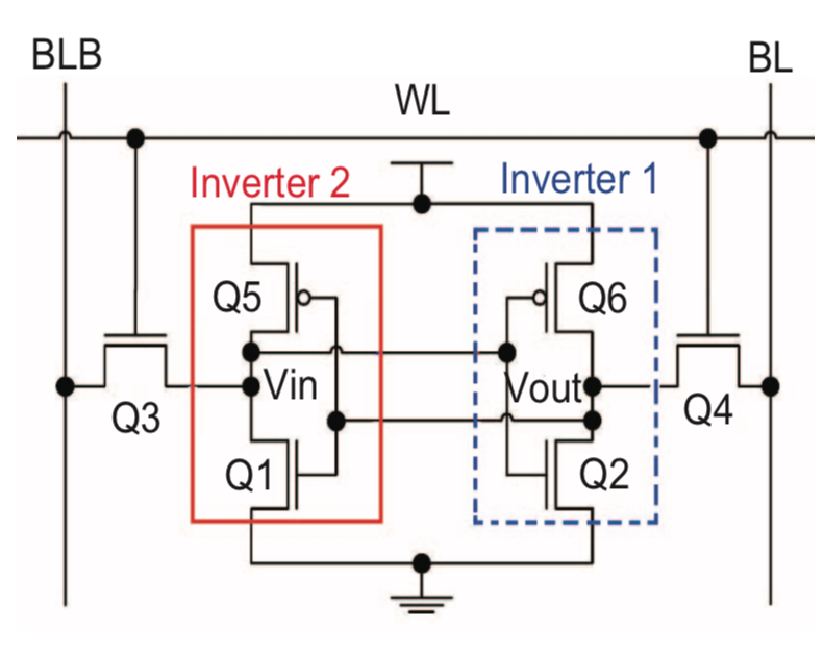
\includegraphics[width={0.5\textwidth}]{images/sram_cell}}
    \caption{A 6-T CMOS SRAM cell \cite{modeling_sram}.}
    \label{fig:sram_cell}
\end{figure}

During manufacturing, there are small differences between each SRAM cell due to process variation which leads to a mismatch in the cell \cite{dargar_2011}. This mismatch also means that the two inverters will always behave distinctly. The mismatch itself does not disturb the normal storage functionality of SRAM cell. Based on this bias, SRAM cells can be classified into three categories as shown below \cite{dargar_2011}:
\begin{enumerate}
\item Non-skewed cell\newline
A non-skewed cell has no preference during its startup due to the impact of process variations does not cause any mismatch between the two inverters. This cell has a heavily fluctuated start-up value depending upon the noise introduced in the system.
\item Partially-skewed cell\newline
A partially-skewed cell has a small mismatch between the inverters which lead to a preference over value '0' or '1' but the cell can flip its value upon variation in external parameters.
\item Fully-skewed cell\newline
A fully-skewed cell is a heavily mismatched SRAM cell in a way that the cell inclined towards value '1' or '0' and has a resistance against external influence/noises.
\end{enumerate}

In ideal SRAM PUF scenario, the utilized SRAM cells should be fully-skewed. Fully-skewed cells lead to a guarantee that the PUF response of a given challenge will have small or no difference even though noises present.


\subsection{Problem: Noise}\label{ch:sram_noise}

Similar to most electronic components, SRAM PUF is also affected by any external influence/noises. These noises will flip unstable bits inside the SRAM PUF. Below are some factors presenting noises:

\begin{itemize}
\item Voltage\newline
The noise introduced by voltage is called power supply noise \cite{wang_tehranipoor_2010}. This noise is related to changes in the delay characteristics of the gate. The changes will occur when there are switchings in the circuit after the device is turned on which increase dynamic power and cause a voltage drop on power lines and voltage increase on ground lines.
\item Temperature\newline
Temperature variation can be introduced by the surroundings or voltage variation. The preference of a cell inside SRAM has a high probability to be affected by temperature \cite{dargar_2011}.
% Temperature affects more than voltage on bit flipping.
\item Crosstalk\newline
Crosstalk appears when a signal transmitted on a circuit introduces unwanted side effects in another circuit. Crosstalk happens due to a tight gap between the SRAM cell (tiny interconnect spacing and width). This event becomes more popular due to wider use of faster-operating speeds and smaller geometries (advancement in nanometer technologies) which lead to higher density. Crosstalk is a major contributor to signal integrity problems in modern designs \cite{wang_tehranipoor_2010}. In addition, higher density in SRAM also influences how environments affect SRAM performance (more prone to voltage and temperature difference) \cite{Abu-Rahma2013}.
\item Aging\newline
Aging is related to changes in the silicon after usage for a long time \cite{rao_mahmoodi_2011}. There are three main effects related to the aging of a circuit; time-dependent dielectric breakdown (TDDB), bias temperature instability (BTI) and hot carrier injection (HCI) \cite{Maricau2013}. TDDB is associated with the creation of a conduction path through the gate transistor structure which causes an increase in power consumption and the circuit delay \cite{impact_mosfet}.
BTI causes a degradation of the transistor threshold voltage \cite{temporal_performance}.
HCI generates a change in the transistor threshold voltage \cite{impact_hot_carriers}. HCI is caused by a high current in the transistor channel injecting charges into the gate oxide during the switching.
\end{itemize}

\subsection{Bit Selection Algorithm} \label{lbl:bit-selection}
As mentioned before, during enrollment, challenge-response pairs are gathered. In SRAM PUF, there are two types of challenges that can be applied to the system. The challenge can be either the whole SRAM memory or specific addresses. If a set of addresses is given as a challenge, an address in there can refer to an address of a byte, a bit, or a sequence of bytes or bits.

If specific addresses of SRAM cells are used for PUF challenge, one of the major steps on using SRAM PUF is looking for stable bits. Stable bits itself refers to fully skewed cells explained before.
Even though the error correction code is present to correct the noise of bit responses, it also has a limitation on how many bits it can correct.
% Since not every SRAM cell is stable, one should take a special caution on deciding which SRAM cell is gonna be the bits to use as PUF input.
Choosing the most stable bits is important to ensure that the PUF result is always the same throughout its lifetime.
Below we present two known algorithms to search for stable bits:
\begin{enumerate}
  \item Neighbor Analysis\newline
The first algorithm is using the rank of total stable neighbors which proposed by Xiao et. al. \cite{xiao_rahman_forte_huang_su_tehranipoor_2014}. They argue that the cells which are “most stable” across environmental conditions are surrounded by more stable cells during enrollment. A stable cell surrounded by more stable cells has a tendency to become more stable because its neighboring cells are likely to experience similar aging stress and operating conditions.
In this algorithm, all the stable cells are given weight according to the number of stable bits surrounding it.
The more stable neighbor cells it has, the higher weight it gets. For example, if a cell is not stable, it is given zero as its score. If it is stable, at least it will get score one. If it only has one stable neighbor on each left and right side, it will get score two as result of an addition of one from being a stable cell and one from having a stable neighbor on both sides. To get score three, it needs to be stable and has two stable neighbors on left and right sides.
After determining the weight of each cell, a heuristic algorithm that greedily chooses cells for the PUF ID/key with weight greater than a threshold is used.

Before the algorithm is performed, one should collect lots of SRAM cells value first. The data should be retrieved in various condition, for example, different voltages, temperatures, and time differences between enrollment.
Afterwards, using the data gathered, the location of all stable bits in SRAM need to be located. A stable bit has to has the same value in all enrollment.
Last, the neighbor analysis algorithm is performed to get the most stable bits in SRAM.

\item Data Remanence Approach\newline
Another bit selection algorithm is by using data remanence of SRAM cell \cite{liu_zhou_tang_parhi_kim_2017}.
There are only two remanence tests involved in this approach: first, writing a value (‘1’ or ‘0’) to the whole memory and second, briefly turning off the power until a few cells flip. The most robust cells are the cells which effortlessly flipped when written with the opposite data. Strong 1's are bits that are flipped fast after 0 is written to its location. On the contrary, if 1 is written to a bit location and the bit flipped fast, it means that the bit is a strong 0.
When using this approach, one should carefully determine the temporal power down time. On one hand, if the temporal power down period is too little, then the data will stay in the previously written state. On the other hand, if the temporal power down time is too lengthy, then the data written in the array will disappear and the SRAM values will go back to its uninitialized state.

A significant advantage using this algorithm compared to the previous one is a much shorter time required to locate stable bits. Using neighbor analysis, there are many SRAM values need to be gathered first which might take hours or days. Locating stable bits from hundreds of data probably also take time as well. If data remanence approach is utilized, there is no need to gather many data. One only need to determine the temporal power down required to get strong bits required. Since usually the temporal down period required is less than 0.5 seconds, this analysis only takes few minutes.
\end{enumerate}

\section{PUF Applications}
In this section, we present three applications which are constructed based on PUF technology. The first application is about generating a key using SRAM PUF, the second one is related to secret key binding based on fuzzy commitment scheme, and the last application is secure key storage using optical PUF and coating PUF.

\subsection{Key Generation using SRAM PUF}

In this section, there are two schemes for key generation presented. Both constructions were built by Hyunho Kang et. al. in 2014. The first construction, shown in Figure \ref{fig:cryptographic_key_generation_old}, utilizes random number generator (RNG). In this example, a key is produced by applying SHA256 hash function on a result of XOR operation between PUF response and a random number. The helper data is generated by XOR-ing PUF response with an encoding of a randomly generated number.
This design was perfected in the second design shown in Figure \ref{fig:cryptographic_key_generation}. In the second design, random number generator was removed to make the construction more efficient without affecting the security. In this design, a key is directly generated based on the PUF response while the helper data is created by XOR-ing the encoding result of PUF-generated key with the PUF response.
Both designs use BCH codes as the error correcting codes with block length ($n$) of 255.

\begin{figure}[tph!]
    \centerline{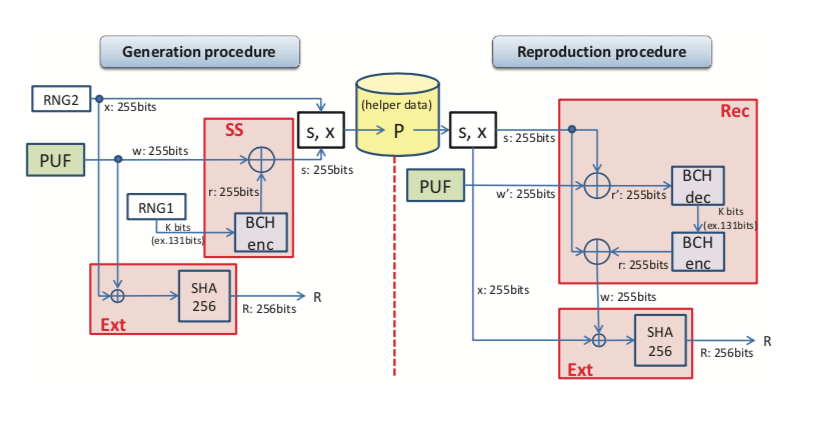
\includegraphics[width={\textwidth}]{images/crypt_key_generation_old}}
    \caption{Implementation diagram using fuzzy extractor (N = 255) \cite{cryptographic_key_generation_old}.}
    \label{fig:cryptographic_key_generation_old}
\end{figure}

\begin{figure}[tph!]
    \centerline{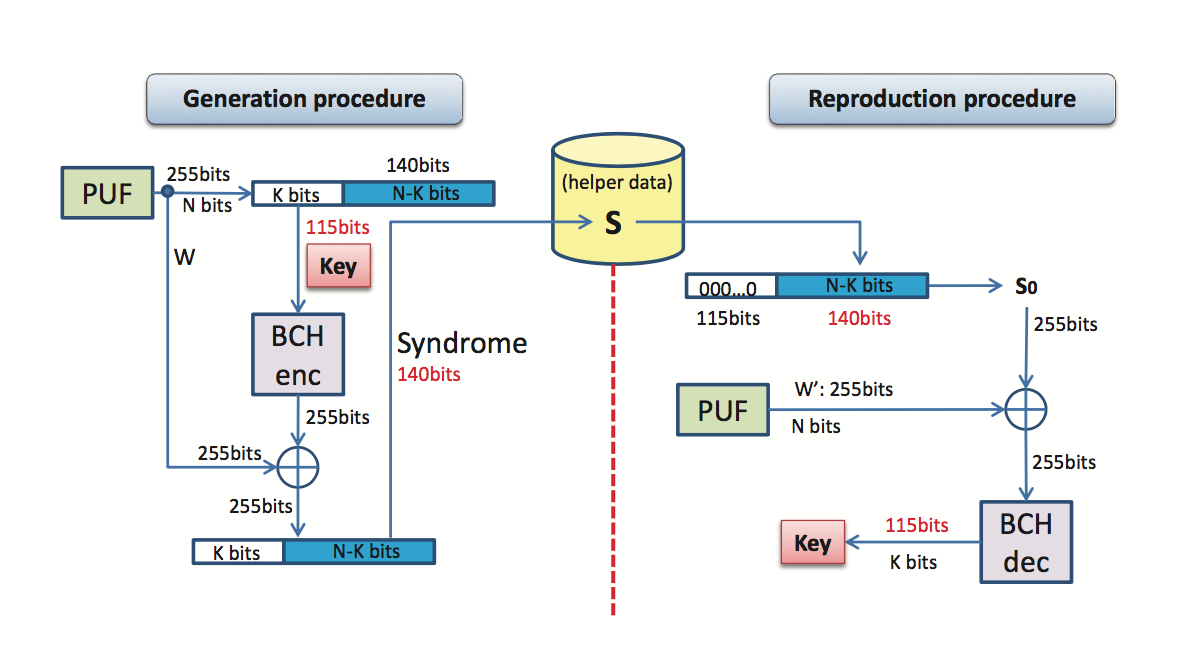
\includegraphics[width={\textwidth}]{images/crypt_key_generation}}
    \caption{Implementation diagram for efficient fuzzy extractor based on the syndrome (N = 255) \cite{cryptographic_key_generation}.}
    \label{fig:cryptographic_key_generation}
\end{figure}

\subsection{Secret Key Binding based on Fuzzy Commitment Scheme}
Fuzzy commitment was originally introduced by Juels and Wattenberg in 1999 \cite{Juels:1999:FCS:319709.319714}. An example of fuzzy commitment application in PUF domain is presented in \cite{8006840}. Figure \ref{fig:fuzzy_commitment} shows the flow of this scheme.
To securely bind the secret, the secret key $S^K$ needs to be chosen first. Afterwards, the secret key is encoded into a binary codeword $C^N$. Then, the helper data $M^N$ is generated by masking (XOR-ing) the codeword with the PUF value $X^N$.
To reconstruct the secret, a noisy version of the codeword $\widetilde{C}^N$ need be calculated by masking the helper data with the noisy version of PUF observation $Y^N$. The secret $\widehat{S}^K$ can be regenerated by decoding the $\widetilde{C}^N$.

\begin{figure}[tph!]
    \centerline{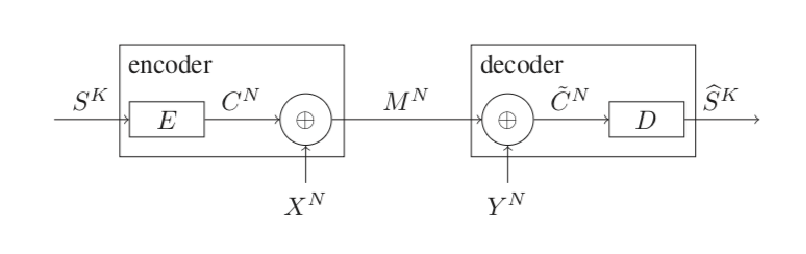
\includegraphics[width={0.8\textwidth}]{images/fuzzy_commitment}}
    \caption{Fuzzy commitment scheme \cite{8006840}.}
    \label{fig:fuzzy_commitment}
\end{figure}


\subsection{Secure Key Storage using Optical PUF and Coating PUF}
In \cite{Skoric2007}, Skoric et. al. present a secure key storage scheme using two extrinsic PUFs; coating PUF and optical PUF. Coating PUF technology is built upon on-chip capacitive quantifications of arbitrary dielectric characteristics of a covering layer which located on top of an IC \cite{10.1007/11894063_29}.  Optical PUF itself consists of a 3-D physical structure containing randomly distributed light-scattering particles that produces a speckle pattern (response) when irradiated with a laser beam \cite{Skoric2007}. This speckle pattern can be considered as the unique fingerprint of the structure. Both PUFs are also considered a strong PUF (has a large CRPs), but optical PUF is considered to be superior than coating PUF due to a much higher number of CRPs and more entropy per response.

% In their scheme, there are two main principle to protect a long term key against physical attacks. First, long term keys should not be stored in non-volatile memory. Second, never let significant portions of the key reside in the volatile memory.
In their scheme, to securely store the key, they proposed to store the long-term key in encrypted form. To access the long-term key, a short-term key extracted from the PUF is required.

\section{Previous Experiments on Off-The-Shelf SRAM PUF}\label{ch:prev_experiments}
There are many experiments related to SRAM PUF which are performed on off-the-shelf SRAM. Most of these experiments are using off-the-shelf SRAM that are embedded in a microcontroller. For example, in \cite{VanHerrewege:2013:DIP:2541806.2512493}, Herrewege et. al. demonstrate a testing of SRAM characteristics on five different microcontrollers; ARM Cortex-A, ARM Cortex-M, Atmel AVR, Microchip PIC16 and Texas Instruments MSP430. They show that not every SRAM embedded in a microcontroller is ideal for an SRAM PUF such as Microchip PIC16F1825. Fortunately, the other microcontroller's SRAMs show an acceptable result to be a PUF candidate (is stable, unique and has enough randomness).
Another example is a work done by Anagnostopoulos et. al. \cite{cryptoeprint:2016:769} in which they present low-temperature data remanence attacks against intrinsic SRAM PUFs, specifically ARM Cortex-M4F LM4F120H5QR microcontroller.

Even though not as many as experiments done on microcontroller's SRAM, there are also some related works that doing the experiments using off-the-shelf SRAM that is not embedded in a specific device. Akhundov in \cite{haji} presents a concept of using SRAM Microchip 23LC1024 as the root-of-trust of his public-key based authentication architecture. He shows the result of HD\textsubscript{intra}, HD\textsubscript{inter} and the distribution of 0's and 1's experiment of Microchip 23LC1024. Unfortunately, the testing was not performed in various condition (different voltage, temperature, and aging effect).
Schrijen and van der Leest in \cite{Schrijen:2012:CAS:2492708.2493033} shows a comparative analysis of seven different SRAMs which manufactured using different technology; Cypress \seqsplit{CY7C15632KV18} (65nm),
Virage HP ASAP SP ULP 32-bit (90nm), Virage HP ASAP SP ULP 64-bit (90nm), Faraday \seqsplit{SHGD130-1760X8X1BM1} (130nm), Virage \seqsplit{asdsrsnfs1p1750x8cm16sw0} (130nm), Cypress \seqsplit{CY7C1041CV33-20ZSX} (150nm), and IDT \seqsplit{71V416S15PHI} (180nm). All of them are tested on the reliability (temperature and voltage variance) and uniqueness (HD\textsubscript{inter} and hamming weight). The results between each SRAM type is different but it can be summarized that all of the tested SRAM memories are suitable as a PUF candidate. Another interesting result from these work is the fact that the most reliable SRAM is achieved by IDT 71V416S15PHI followed by Cypress CY7C1041CV33-20ZSX and Cypress CY7C15632KV18.
Another publication is presented by Holcomb et al. \cite{4674345} where they show start-up measurements from ISSI SRAM, TI microcontrollers, and Intel WISP devices. Unfortunately, the manufacturing technology on these devices is not mentioned.
% Another example is a work done by Zhang et.al in \cite{7459321} where they did an experiment of introducing a novel PUF implementation of the second category that exploits the effect of manufacturing process variations in SRAM read access current
% on SRAM ISSI IS62C256AL to explot Current based PUF Exploiting Random Variations in SRAM Cells


\section{Conclusion}
It is a challenging task to design a secure data and key storage based on SRAM PUF technology, especially since to solve this task, we need to understand the term of software and hardware security. Therefore, we investigate several background theory related to security, cryptography, and PUF. We started by presenting four elements on common security; confidentiality, authentication, integrity, and non-repudiation. Then, the history of cryptography is explained, followed by explanations on symmetric cryptography, key derivation function, and multi-factor authentication.
Later on, theories related to PUF, hamming distance, error correcting codes and SRAM PUF are described. We continue the chapter by a portrayal of several PUF applications, such as key generation and key storage. We also show some previous works which related to SRAM PUF built using off-the-shelf SRAM. In the next chapter, our proposed ideas on how to build a secure data and key storage using SRAM PUF and off-the-shelf SRAM will be explained.

% % \chapter{Related Works}
\chapter{SRAM PUF Applications}

\section{Key Generator}

In this section, there are two scheme for key generation produced by Hyunho Kang et. al. Both constructions were built on 2014. The first construction, shown in \ref{fig:cryptographic_key_generation_old}, is utilizing random number generator (RNG). This design was perfected in the second design shown in \ref{fig:cryptographic_key_generation}. In the second design, random number generator was removed without affecting the security.

\begin{figure}[tph!]
	\centerline{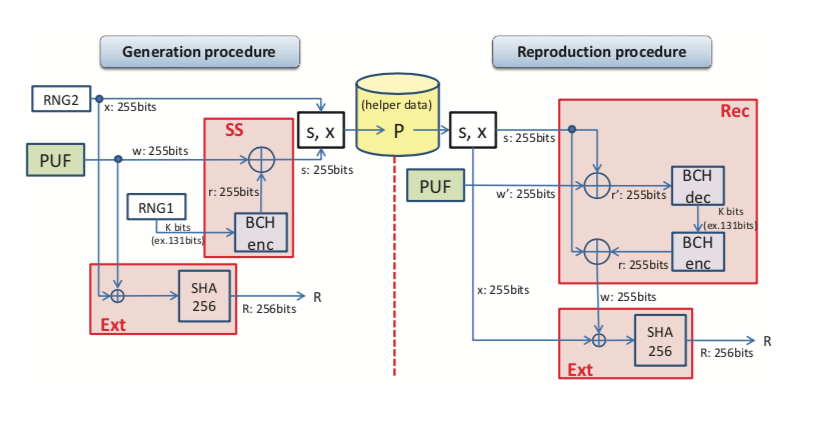
\includegraphics[width={0.5\textwidth}]{images/crypt_key_generation_old}}
% \centerline{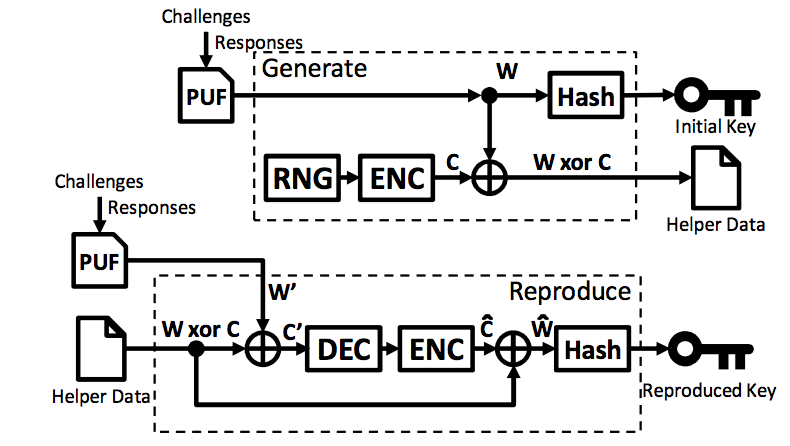
\includegraphics[totalheight=6cm]{images/scheme_stable_key_generation.png}}
    \caption{Implementation diagram using fuzzy extractor (N = 255) \cite{cryptographic_key_generation_old}}
    \label{fig:cryptographic_key_generation_old}
\end{figure}

\begin{figure}[tph!]
	\centerline{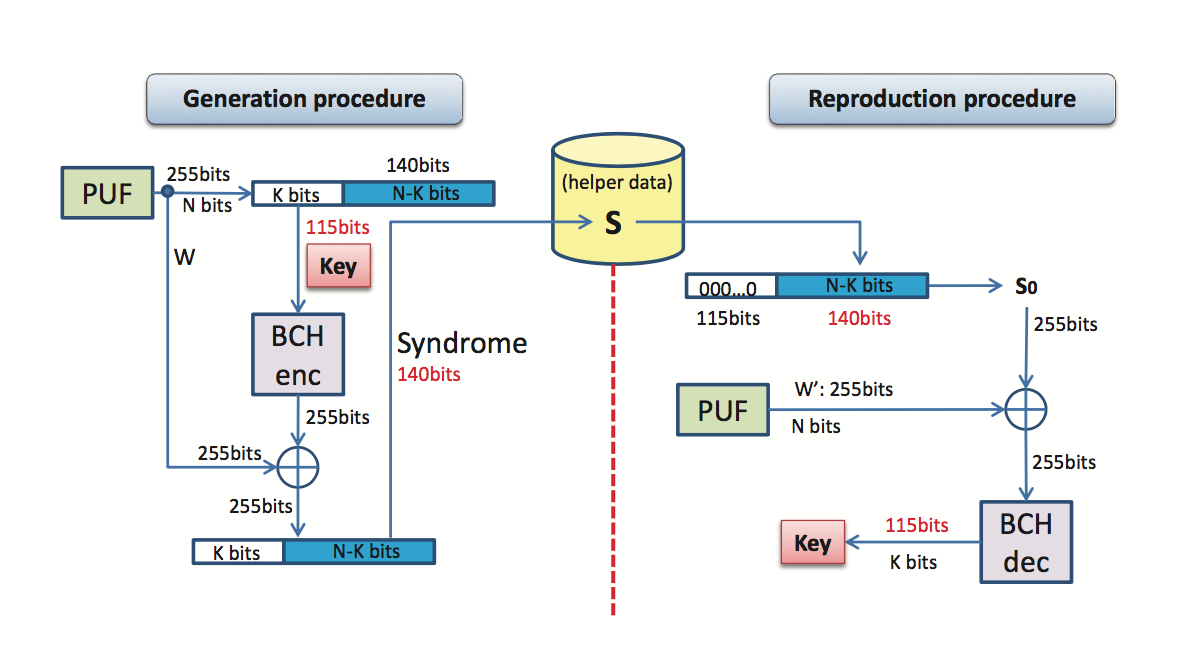
\includegraphics[width={0.5\textwidth}]{images/crypt_key_generation}}
% \centerline{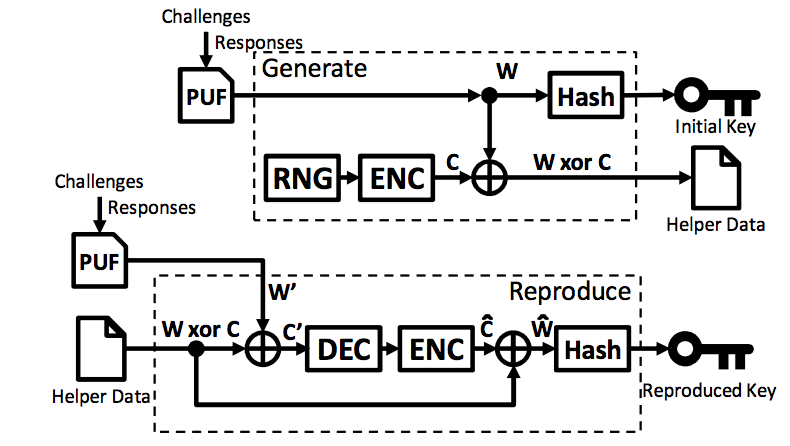
\includegraphics[totalheight=6cm]{images/scheme_stable_key_generation.png}}
    \caption{Implementation diagram for efficient fuzzy extractor based on the syndrome (N = 255) \cite{cryptographic_key_generation}}
    \label{fig:cryptographic_key_generation}
\end{figure}

% \begin{figure}[tph!]
% 	\centerline{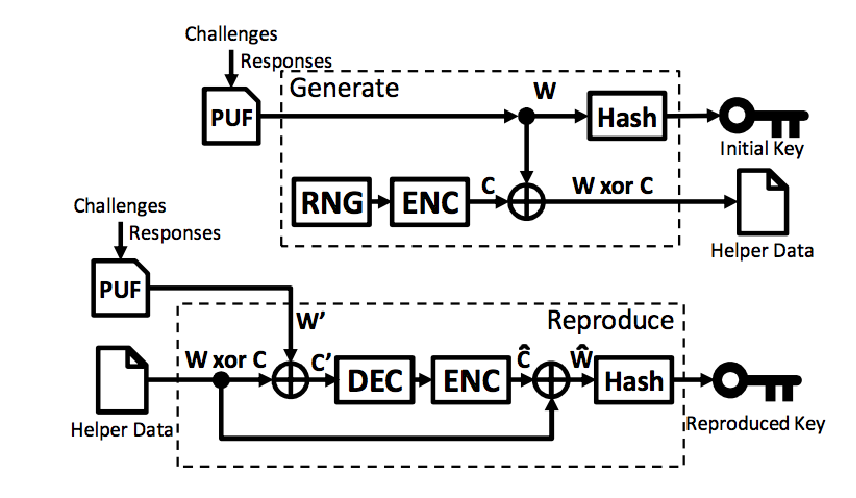
\includegraphics[width={0.5\textwidth}]{images/scheme_stable_key_generation}}
% % \centerline{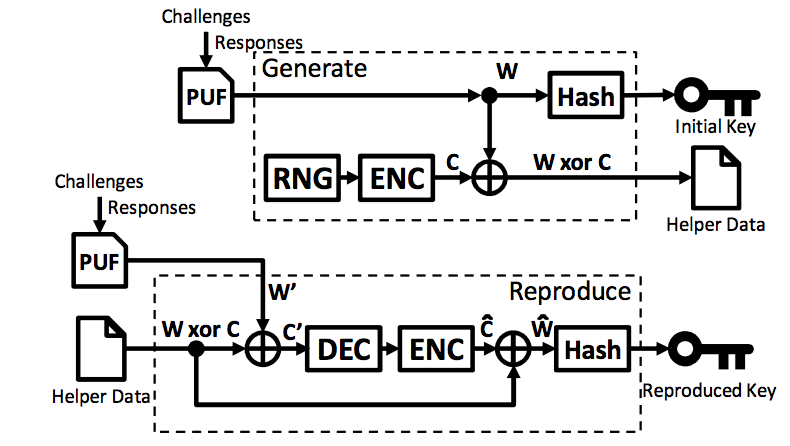
\includegraphics[totalheight=6cm]{images/scheme_stable_key_generation.png}}
%     \caption{Scheme of Stable Key Generation}
%     \label{fig:scheme-key-generator}
% \end{figure}


\section{Key Storage using PUF Scheme}

In a basic key storage scheme using PUF, it usually divided into two phases.  In the first phase, generally called enrollment, the helper data is constructed by XOR-ing PUF bits and the encoded key. In the second phase, which called reconstruction, the helper data is XOR-ed with the PUF bits, followed by decoding the result to reconstruct the key.

% \begin{figure}[tph!]
% \centerline{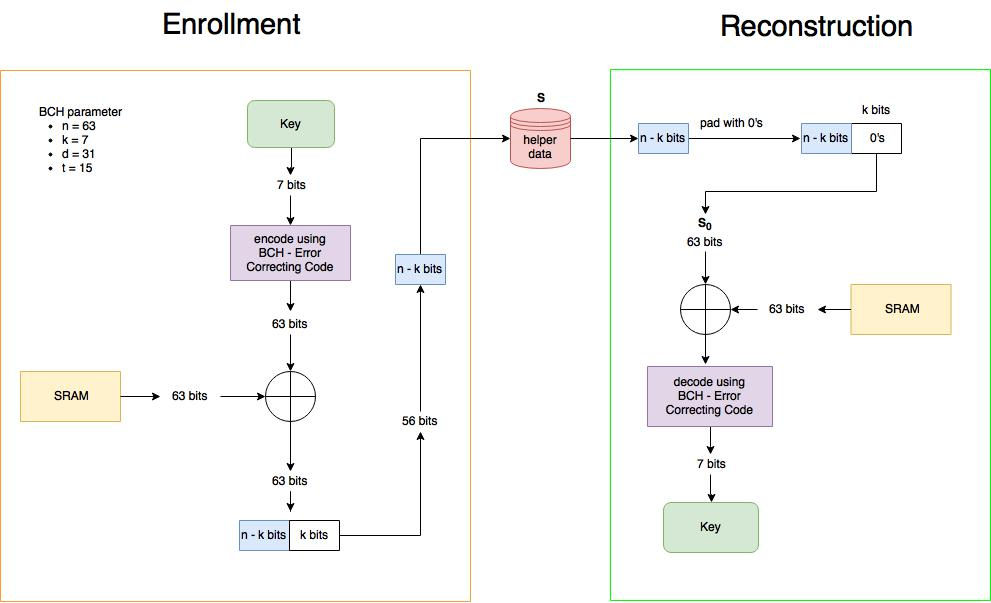
\includegraphics[totalheight=6cm]{images/key-storage-scheme.jpg}}
%     \caption{Scheme for Storing Key}
%     \label{fig:key-storage-scheme}
% \end{figure}


\section{Authentication using PUF Scheme}

In a basic authentication scheme using PUF, it usually divided into two phases.  In the first phase, generally called enrollment, CRPs are generated and stored in a CRP database. In the second phase, usually referred to verification, a challenge from the CRP database is applied to the PUF and the response produced by the PUF is compared with the corresponding response from the database.

% \input{chapter/chapter3}
\chapter{\chapterFour}
\label{chp:4}

\textit{This chapter contains our proposed system to achieved our goals which explained in Chapter 1. First, assumptions, requirements and steps to achieve thesis' main goal. on our system are presented. The chapter continues with reasonings on our chosen embedded platform, Arduino. Then, the selected error correcting code which will be used in the system is explained. Afterwards, we present our data and key storage scheme and also our way to generate key using SRAM PUF. Last, our idea to use bits locations as a PUF challenge is shown. }

\section{Assumptions, Requirements and Steps To Achieve Main Goal}\label{ch:use_case}

% As mentioned in the first chapter, a subset of this thesis goal is to provide a secure data protection and key storage scheme using SRAM PUF. This thesis goal describes the use case of our proposed system.
To focus the thesis approach, we have defined several assumptions. First, the field of the constructed SRAM PUF application is decided to be only available offline. Accessing the SRAM PUF requires the user to have the device next to his/her side. Second, an attacker cannot access the SRAM directly. An attacker may gain the knowledge of the helper data and challenge used in the PUF concept. Last, there is no analysis and/or solution against physical attacks, e.g side channel attacks, in our secure data and key storage scheme. The scheme is designed to be secure against theoretical attacks.

We also have define a set of requirements related to our system. Below are the requirements defined:

\begin{enumerate}
    \item Software-based construction\newline
    There should be no major hardware modification or hardware design to implement the project.
    \item Patent/license free\newline
    Any dependent component of the design should be in public domain.
    \item Open-source and collaboration oriented\newline
    If there's a reliable open source project which can be a foundation for this thesis project, instead of building our own software, it is preferred to use that project. This will significantly reduce the time consumed on constructing the whole project. Using other project source code can also increase the collaboration atmosphere. In addition, this requirement may help this project to be known by others since they might introduce our project as one of the projects that uses their code.
    \item Key-length security level\newline
    The goal on the key-length security level is 256-bits. The concept constructed should be able to use this level and the project's security should be uncompromised even though the key-length is only 256-bits.
    \item Off-the-shelf SRAM\newline
    The SRAM involved in the thesis should be easily available in the market and cost insignificant.
    \item Affordable\newline
    The total hardware required to produce the system should be inexpensive.
    \item Reproducible\newline
    Anyone should be able to reproduce this thesis experiment with no significant effort.
\end{enumerate}

Another thing that we would like to address is steps required to achieve this thesis' main goal which related to answering this thesis' problem statement. As shown in Section \ref{ch:problem}, the problem statement is "\problemStatement".
Below are several steps expected to be done as an attempt to achieve this goal:
\begin{enumerate}
  \item Choose embedded platform on where the system will be built.
  \item Select a type of error-correcting codes which will be used as an element in the key generation scheme. The memory required by the error correcting codes has to fit in the embedded platform's internal memory.
  \item Search and analyze existing SRAM PUF-based key generation schemes. Propose one of them to be used as the key generation procedure in this thesis and also calculate the maximum error rate that can be handled by the key generation scheme.
  \item Propose and construct a system to enable secure data and key storage based on the selected key generation scheme and SRAM PUF technology. Any library required in the system has to be open-source. In addition, the constructed system has to work without any explicit hardware design, in other words, \textit{software-based} construction.
  \item Get off-the-shelf SRAM components available in the market.
  \item Locate the stable bits inside each SRAM using bit selection algorithm.
  \item Test the reliability of SRAM's stable bits. The error rate of the stable bits (referred as HD\textsubscript{intra}) has to be lower than the maximum error rate that can be handled by the key generation scheme.
  \item If the SRAM's stable bits is reliable, continue using this SRAM as the root-of-trust in the proposed secure data and key storage.
  \item Test the complete secure data and key storage scheme in various scenarios.
\end{enumerate}

\section{Arduino Mega 2560 as the Embedded Platform}

One of the important details of our system is choosing the platform on where the system will be built.
There are two major candidates, Arduino and Raspberry Pi. Both are chosen due to its popularity, availability (easy to get), and various types available. High popularity means the debugging process can be done fast and many references are available online to help the system development. Availability is important because this thesis goal should be easily used by anyone. Low availability will reduce significantly reusability of this project and user's interest. Various types available is a good option for system flexibility. For example, if a user wants to develop a more complex system on top of this thesis' system or desire to use a more complex error correcting codes, he/she can choose a platform with higher computing capability.
Besides those three factors, another feature which lead on selecting Raspberry Pi and Arduino is their GPIO. GPIO availability will enable easy communication between the SRAM and the embedded platform.

Compared to Arduino, Raspberry Pi offers a higher computing capability and relatively easier development. This is because Raspberry Pi is basically a mini Linux computer. One can develop a software using C, C++, Python, etc. in Raspberry Pi which may fasten the project development, especially for a developer who already familiar with a specific programming language. Unfortunately, Raspberry Pi requires a longer startup time compared to Arduino. It also requires higher electrical power. If one wants to use the developed project in the embedded area, this two factor is a major trade-off.

Due to the above consideration, Arduino is chosen. Even though one has to construct the system in C++, this can be a positive thing since one can maximize the computing capability easily. Moreover, Arduino itself is an open-source project which enable anyone to develop their own boards and software libraries \cite{arduino}.

There are various Arduino types available on the market. The chosen Arduino type is Arduino Mega 2560. It is selected because it offers larger memory capability compared to other types, such as 256k bytes of Flash memory, 8k bytes internal SRAM, and 4k byte EEPROM.
Besides, it also has 54 digital I/O pins and 16 analog I/O pins which ease the communication to external SRAM.

\section{BCH Codes as Error Correcting Codes}
As shown in previous chapter, there are two major categories in ECC; soft-decision and hard-decision code. We choose to use hard-decision ECC over the soft decision one since there is no requirement to provide the error probability function on SRAM cells. Futhermore, between two examples of hard-decision ECC, we particularly pick BCH codes as the ECC due to lower computing resource required compared to Reed-Solomon Codes. BCH also better at correcting random errors than Reed-Solomon Codes.

As mentioned in the previous chapter, BCH codes are flexible Error Correcting Codes (ECC) shown by multiple parameters available. The only fixed parameter is $q$ since the problem is in binary form ($q=2$). The source code for BCH codes utilized in our construction is a modified version of Robert Morelos-Zaragoza's version which can be retrieved at \cite{bch_code}. This code is selected because it can support $m$ ranging from 2-20 which mean the length of the code that can be corrected ranging from 2 until 1048575. When using BCH codes, one should be careful on deciding the parameters that will be used, for example, larger $m$ or $n$ means a bigger memory needed.
These parameters should be determined with several considerations, such as the inner hamming distance of SRAMs and memory available on Arduino Mega 2560.

On deciding the value $m$, a further look on the memory required during the error correction computation need to be done. Inside the bch codes from \cite{bch_code}, the decoding method requires the largest memory compared to other procedures. There are six parameters that depend on $m$ which are $elp$, $d$, $l$, $u_lu$, $s$, and $err$. Table \ref{tab:memorybch} shows the required memory given the $m$ value.

\begin{table}[htbp]
  \centering
  \caption{Memory required (bytes) given the value of $m$.}
    \begin{tabular}{|l|l|l|l|}
    \hline
    \multicolumn{1}{|c|}{\textbf{m}} & \multicolumn{1}{c|}{\textbf{Bytes Required}} & \multicolumn{1}{c|}{\textbf{m}} & \multicolumn{1}{c|}{\textbf{Bytes Required}} \\
    \hline
    2     & 53    & 12    & 16805897 \\
    \hline
    3     & 129   & 13    & 67166217 \\
    \hline
    4     & 377   & 14    & 268550153 \\
    \hline
    5     & 1257  & 15    & 1073971209 \\
    \hline
    6     & 4553  & 16    & 4295426057 \\
    \hline
    7     & 17289 & 17    & 17180786697 \\
    \hline
    8     & 67337 & 18    & 68721311753 \\
    \hline
    9     & 265737 & 19    & 274881576969 \\
    \hline
    10    & 1055753 & 20    & 1099518967817 \\
    \hline
    11    & 4208649 &       &  \\
    \hline
    \end{tabular}%
  \label{tab:memorybch}%
\end{table}%

Since the internal SRAM in Arduino only has 8k bytes capacity, the chosen $m$ is 6 (requires 4553 bytes, around 55\% of total SRAM available in Arduino). This parameter will result in possible $n$ between 32 and 63. $n$ is chosen to be 63 to maximize the length code that can be encoded.
The combination of $m$ = 6 and $n$ = 63 results in various $k$ and $t$ that can be chosen. The combination of all parameter possible is shown on \ref{tab:bch}.

\begin{table}[htbp]
  \centering
  \caption{BCH parameter for $m$ = 6 and $n$ = 63.}
    \begin{tabular}{|r|r|}
    \hline
    \multicolumn{1}{|c|}{\textbf{k}} & \multicolumn{1}{c|}{\textbf{t}} \\
    \hline
    \multicolumn{1}{|l|}{57} & \multicolumn{1}{l|}{1} \\
    \hline
    51    & 2 \\
    \hline
    45    & 3 \\
    \hline
    39    & 4 \\
    \hline
    36    & 5 \\
    \hline
    30    & 6 \\
    \hline
    24    & 7 \\
    \hline
    18    & 10 \\
    \hline
    16    & 11 \\
    \hline
    10    & 13 \\
    \hline
    7     & 15 \\
    \hline
    \end{tabular}%
  \label{tab:bch}%
\end{table}%
To maximize the error correction capability, $k$ = 7 and $t$ = 15 is chosen. All these parameter combination will enable error correction capability 23.8\% of the data length. To summarize, here are the chosen parameters:
\begin{itemize}
\item $n$: 63
\item $k$: 7
\item $d$: 31
\item $t$: 15
\end{itemize}

\section{Data and Key Storage Scheme} \label{chp:data_protection_scheme}

Figure \ref{fig:scheme-data-protection} shows the scheme to protect user's data and key. On an attempt to protect the user's data and key, our proposal is divided into three major parts, first is generate the final key, and the rest is using the final key either to encrypt or decrypt data.
To prevent unauthorized person accessing the data with a stolen PUF, an idea from multi-factor authentication is utilized. Instead of just depending on the PUF device to access the key, a combination of PUF device and user knowledge is presented. User knowledge that used here is password.
User's password is combined with the PUF-generated key to generate a \textbf{final key} using HMAC. The input message to the HMAC is the user's password and the input key to the HMAC is the PUF-generated key. The HMAC function proposed to use is HMAC-SHA3 with key length 256 bits.
The final key can be used to encrypt and decrypt user data/key. To decrypt and encrypt the data, a symmetric encryption algorithm is preferred over the asymmetric one. The symmetric encryption algorithm used is AES with key length 256 bits.

\begin{figure}[tph!]
    \centerline{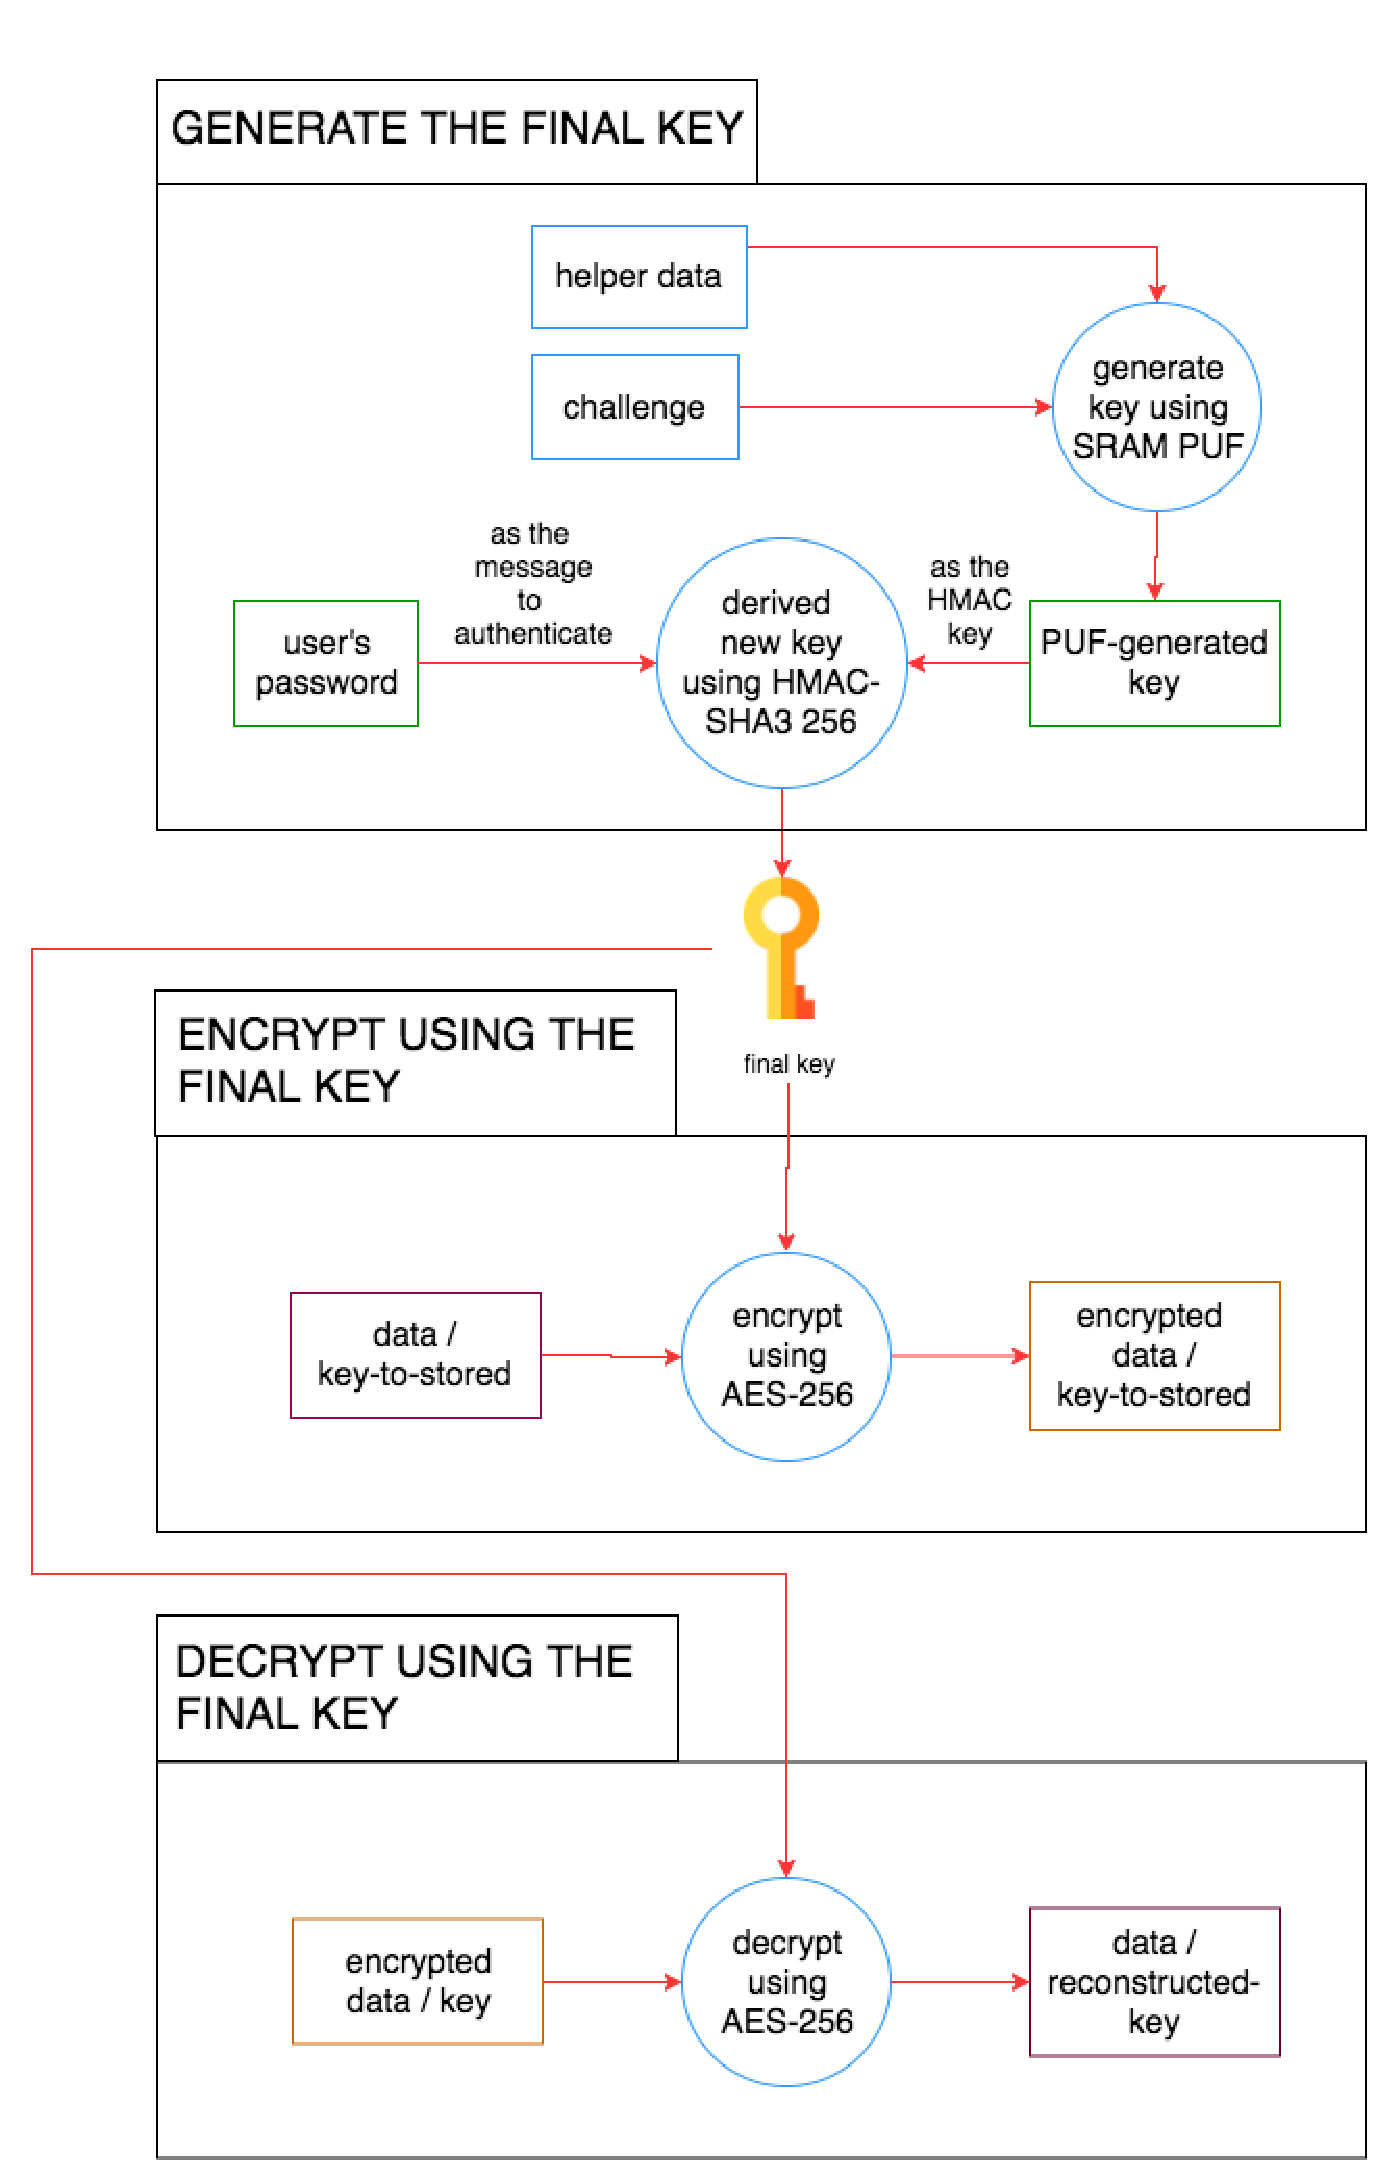
\includegraphics[width={0.9\textwidth}]{images/proposed}}
    \caption{Scheme for secure data and key storage. There are three stages in here; generate the final key, encrypt using the final key and decrypt also using the final key.}
    \label{fig:scheme-data-protection}
\end{figure}

% We believe this scheme is secure due to several assumption.
% First, if the attacker decides to attack the scheme by applying a cryptanalysis directly to the ciphertext, the attacker has to break the security level of AES-256. If brute-force attack is applied to AES-256, the attacker has to try all possibilities of $2^{256}$ keys which roughly equals to $1.157920892373163 \times 10^{77}$. Even if one can try ten thousands keys every second, the total time needed to try all combinations is still $3.67 \times 10^{65}$ years (longer than the age of the universe which is $14 \times 10^9$ years old).
% The attacker may also apply key-recovery attack using a technique called biclique attack \cite{10.1007/978-3-319-19962-7_3}. Even though this technique is the best known attack on AES-256, this technique still requires time complexity of $2^{254.27}$ and data complexity of $2^{40}$.

\section{Key Generation Scheme}

As shown in the previous section, the secure data and key storage scheme requires the PUF to generate the key which will be used to generate the final key. The key generation scheme used in this project is a modified version of Figure \ref{fig:cryptographic_key_generation} proposed in \cite{cryptographic_key_generation}. Instead of using $n$ = 255, the scheme used in this project will choose $n$ = 63. The parameter \textit{n, k, t, d} is similar to the parameter chosen in the previous section, BCH error correcting code. Figure \ref{fig:key-generation-scheme} illustrates the mentioned scheme.
Using this scheme, to generate a key with length 256-bits requires 37 blocks of this scheme, which lead to 2331 bits required. 37 blocks are calculated from $256\div7=36.57$, rounded-up resulting in 37. 7 comes from the key generated from 63 bits of data using this scheme. Since one block needs 63 bits of data, 37 blocks require $37\times63=2331$ bits.
In addition, if you look further into the scheme, there is an entropy loss as many as 7 bits every 63 bits input during the generation of helper data. Due to this entropy loss, this scheme can only correct errors on maximum 8 bits instead of 15 bits. Based on this reason, to ensure the key generation scheme always produced the same key, the SRAM component used as root-of-trust has to have maximum error rate (shown by HD\textsubscript{intra}) 12.7\% (calculated from $8\div63\times100\%$).

\begin{figure}[tph!]
    \centerline{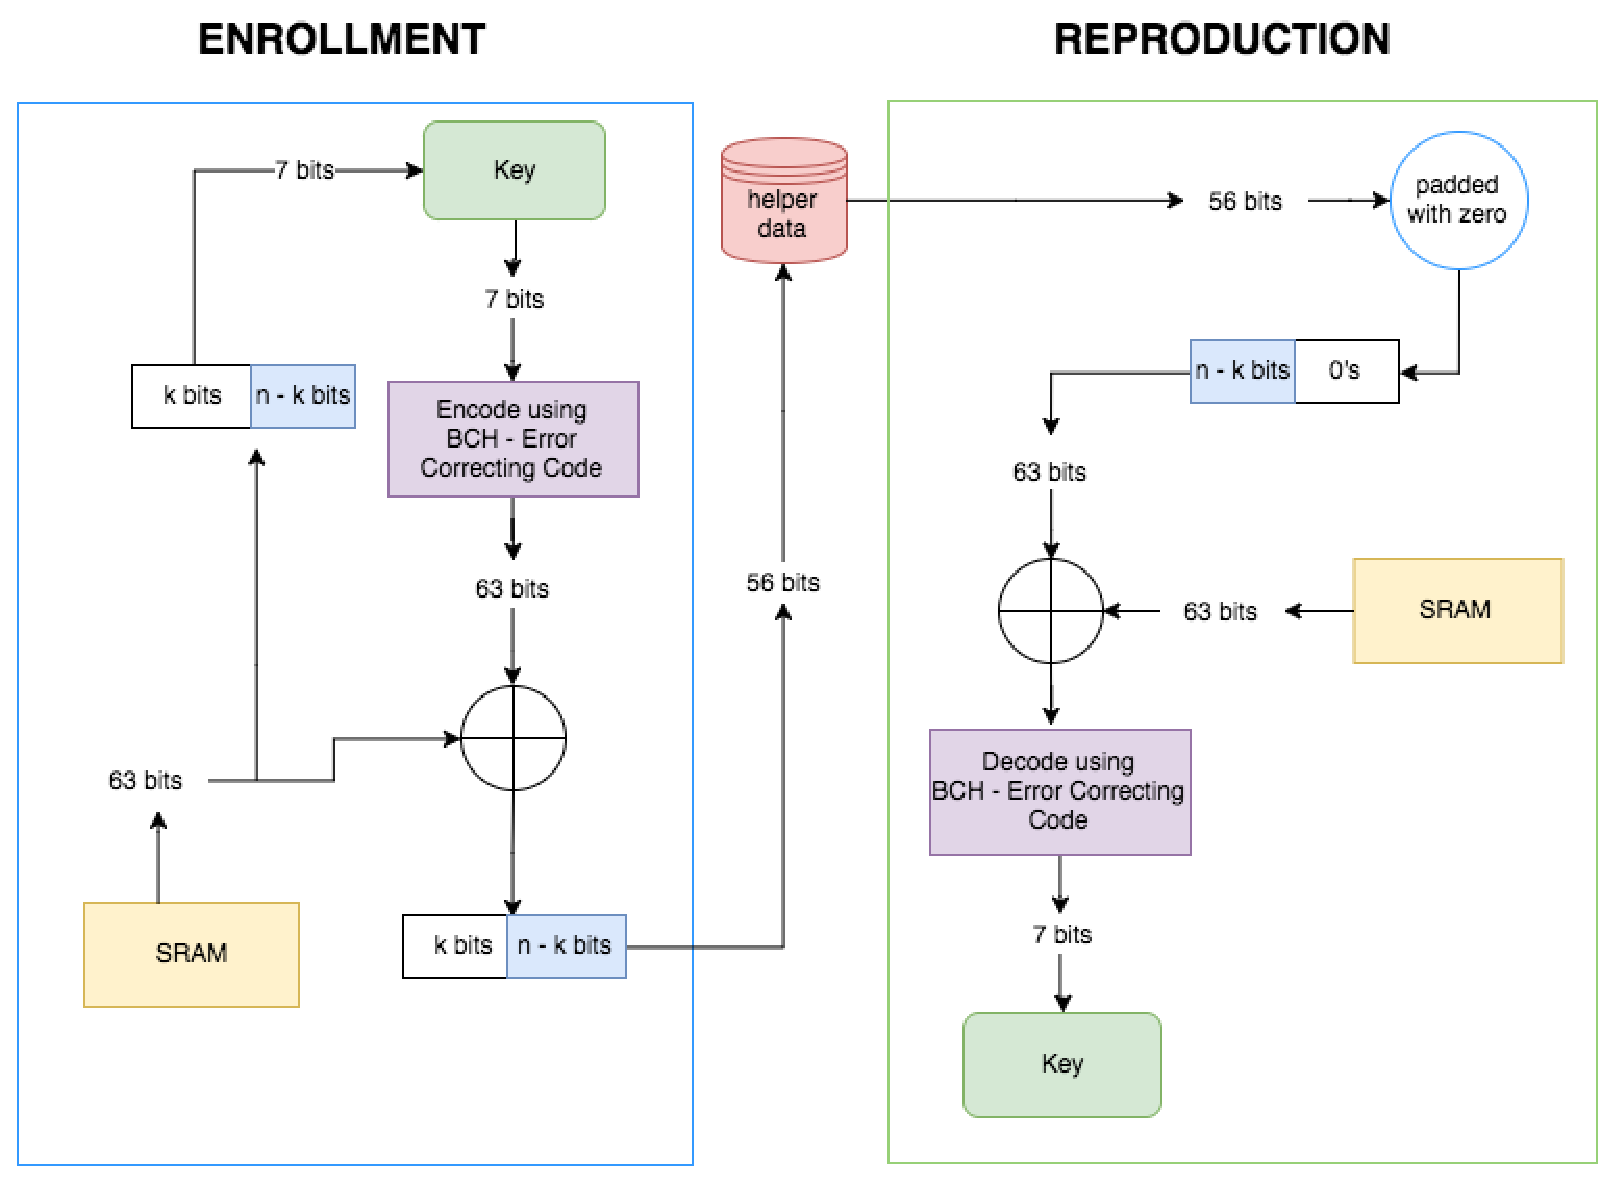
\includegraphics[width={\textwidth}]{images/key}}
    \caption{Scheme for key generation. $n$ = 63, $k$ = 7, $t$ = 15, $d$ = 31.}
    \label{fig:key-generation-scheme}
\end{figure}


\section{Bits Locations as the PUF Challenge - Numerous CRPs}
An example of a well known PUF construction which claimed to be resistant against brute force attack is Stanzione and Iannaccone's work \cite{Stanzione}. They mentioned that their PUF construction is resistant to $10^{25}$-trials brute force attack. Inspired by their work, we imagine having a stronger construction. We envision an SRAM PUF which has total challenge-response pairs possibilities more than the number of atoms on earth which predicted to be at least $10^{49}$ \cite{atoms_earth}. To achieve this goal, we come up with an idea to use bits locations as a PUF challenge.
Below are the reasons why this decision is taken:
\begin{enumerate}
    \item Stable bits tend to be scattered all around SRAM memory.
    \item If there's a burst error on a bit location inside the challenge, this error will not affect many locations in a challenge since this burst error may only lead to a single location. If a location related to multiple bits is used as the challenge, a burst error will affect many bits generated. For example, if locations of bytes are used as the challenge, a burst error might lead to 8 bits errors in the response generated.
    \item There are huge possibilities of challenge-response pairs. The number of possibilities is calculated from the \textit{permutation} of the required bits and the available bits using Equation \ref{bits}.
    \begin{equation}
        \label{bits}
        P(n,r)=\frac{n!}{\left( n-r \right) !}
    \end{equation}
\end{enumerate}
As an illustration, if the number of bits required to generate/reconstruct the key is 2331 bits (the length of the bits required to generate 256-bits key when using scheme shown in Figure \ref{fig:key-generation-scheme}), then a set of 2331 bits locations is required as an input (a challenge) to PUF device. And if the SRAM has a total capacity of 65536 bits, using Equation \ref{bits} explained before, there are $P(65536, 2331)=\frac{65536!}{\left( 65536-2331 \right) !}\approx 10^{11209}$ possible combinations. The total possible CRPs is even much higher compared to the total possibilities of the number of bits required ($2^{256}\approx5.02\times10^{701}$) or the number of possible keys ($2^{256}\approx1.16\times10^{77}$).
Due to these large possibilities of challenge-response pairs, this idea will lead to \textbf{numerous CRPs}.
% Due to these large possibilities of challenge-response pairs, this idea will lead to a \textbf{strong PUF} (as mentioned in section \ref{lbl:puf-classification}, a strong PUF can be identified by having a large number of CRPs).

Using this concept, before generating the challenge, the location of stable bits needs to be identified first. The location of stable bits can be detected by using bit selection algorithm mentioned in section \ref{lbl:bit-selection}.
After the location of stable bits is identified, during the generation of a challenge, the locations' order inside the challenge will be randomized.

\section{Security Analysis of The Proposed Scheme}
As mentioned in Section \ref{ch:use_case}, our scheme is designed to be secure against theoretical attacks. There are three elements in our scheme as the main parts on ensuring the scheme's security against such attacks; encryption using AES-256, key derivation function using HMAC SHA3-256, and the PUF-generated key. Based on these components, the attack scenarios are presented below:
\begin{itemize}
  \item The simplest way of attacking the scheme is by applying a cryptanalysis directly to the ciphertext produced by the scheme. If successful, this attempt will result in known final key used in the scheme and the plaintext.  In this way, the attacker has to break the security level of AES-256. If brute-force attack is applied to AES-256, the attacker has to try all possibilities of $2^{256}$ keys which roughly equals to $1.157920892373163 \times 10^{77}$. Even if one can try ten thousand keys every second, the total time needed to try all combinations is still $3.67 \times 10^{65}$ years (longer than the age of the universe which is $14 \times 10^9$ years old).
  The attacker may also apply key-recovery attack using a technique called biclique attack \cite{10.1007/978-3-319-19962-7_3}. Even though this technique is the best-known attack on AES-256, this technique still requires time complexity of $2^{254.27}$ and data complexity of $2^{40}$.
  \item Another attempt that may be taken by the attacker is by stealing the PUF device. Even though the attacker has the PUF device, he still cannot access the encrypted data directly since he has to guess the PUF owner's password. If PUF owner's password entropy is high enough, the chance for attacker to successfully gain the access to the encrypted data is small since he basically has to break the security level of HMAC SHA3-256 (which requires at least $min(2^k, 2^n)$ time complexity, where $k$ is the key size and $n$ is the hash output size. \cite{hmac_security}).
  \item The attacker may also try accessing the encrypted data by doing a social engineering to gain the information of PUF owner's password, then guess the PUF-generated key to get the final key which used to encrypt the data. To successfully predict the PUF generated key, it is also a hard work. For example, if one want to brute force all possible input combinations to the PUF key generation scheme, there are $2^{2331} \approx 5.02 \times 10^{701}$ possible combinations. It is actually easier to just try all possible combinations of the PUF-generated key which has 256-bits in length. Even though such fact exists, the number is not small either. The total possibilities still accounts for $2^{256}$ keys which roughly equals to $1.157920892373163 \times 10^{77}$ possibilities.
\end{itemize}
Based on these reasonings, we believe our proposed data protection and key storage scheme is secure. The only possible way for an attacker to gain information from the encrypted data is by having both PUF device and PUF owner's password.

% security of the schemes
% - relies on AES 256
%   - key generated using SHA3-256
%
% security of the bits locations as challenges

\section{Conclusion}
After presenting related works in previous chapter, this chapter continues with explanations of our proposed ideas to answer the thesis' problem statement and achieve our goals which explained in Chapter 1. In the beginning, use cases, assumptions, requirements and steps to achieve the thesis' main goal on our system are presented.
The chapter continues with reasonings on our chosen embedded platform, Arduino. Specifically, we choose a product type of Arduino called Arduino Mega 2560 because it offers larger memory capability compared to other types and has 54 digital I/O pins which ease the communication to external SRAM.
Then, the selected error correcting code which will be used in the system is explained. We choose to use hard-decision ECC over the soft decision since there is no requirement to provide the error probability function on SRAM cells. Between two examples of hard-decision ECC, we particularly pick BCH codes as the ECC due to lower computing resource required compared to Reed-Solomon Codes. BCH also better at correcting random errors. The parameter used in our BCH codes are $n$: 63, $k$: 7, $d$: 31, $t$: 15.
Afterwards, we present our secure data and key storage scheme. To secure the data, we encrypt the data with a final key which derived using HMAC SHA-3 256 as a KDF with input PUF-generated key and user password. To produce the PUF-generated key, we choose to use a modified version of key generation scheme proposed in \cite{cryptographic_key_generation}.
We continue by presenting our idea to use bits locations as a PUF challenge. Our proposed PUF challenge are based on the permutation of stable bits which lead to a numerous number of possibilities.
Last, we present security analysis of the proposed secure data and key application. There are three elements as the main parts of ensuring the security goal; encryption using AES-256, key derivation function using HMAC SHA3-256, and the PUF-generated key. Based on three elements, we displayed three different attack scenarios.
In the next chapter, the experiments done in this thesis will be explained.

% \chapter{Experiment}
\chapter{\chapterFive}
\label{chp:5}

\textit{After describing our proposed system as an attempt to achieve this thesis' goals in the previous chapter, this chapter continues with an explanation of several experiment setups and results. This chapter starts by a presentation on two chosen SRAMs that used in experiments; Microchip 23LC1024 and Cypress CY62256NLL. Afterwards, the testing results on two bit selection algorithms (neighbor analysis and data remanence approach) and the stable bits produced by these algorithms are displayed. The chapter continues with examination on our proposed PUF challenge and a presentation on our complete enrollment scheme. Then, we present the procedure to develop SRAM PUF-based applications using any off-the-shelf SRAM.
Next, testing on the designed secure data and key storage scheme is shown. Experiment outcomes on storing Bitcoin private key will conclude this chapter.}

\section{Chosen Off-The-Shelf SRAMs}
The first step to do in this thesis implementation is looking for off-the-shelf SRAM components to be the root-of-trust in our SRAM PUF project.
Due to numerous SRAM types available in the market, we need to define several requirements for the SRAM first. The main requirements on the SRAM are easy to get (a simple Google search should show some e-commerce websites to buy from), can be bought in small quantity ($\leq$ 5 pieces), stand-alone component (available without buying extra component, e.g. not embedded in an FPGA), inexpensive (cost less than \euro{}5), reasonable memory size ($\geq$ 64kb). These criteria are chosen due to some products only sold to a company or an entity that willing to buy in a big quantity or has to be custom made. There are two SRAM types purchased and tested here; Microchip 23LC1024 and Cypress CY62256NLL.

% As mentioned in Chapter 2, to be qualified as a PUF candidate, an SRAM has to be stable in various conditions. This means if it is given various power input or used in varied temperatures or utilized for a long time, the initialized SRAM values has to remain similar or only has little changes. Under any condition, there should be no overlap between HD\textsubscript{intra} and HD\textsubscript{inter}. Moreover, the SRAM has to have a sufficient amount of randomness, shown by having equal distributions between 1's 0's on its values.  To ensure the quality of these two SRAMs, there are several experiments performed on each SRAM, such as calculating HD\textsubscript{intra} and HD\textsubscript{inter} given the whole memory value as the challenge and also the distribution of 1's and 0's inside SRAM memory.
%
\subsubsection{Microchip 23LC1024}
The Microchip Technology Inc. 23A1024/23LC1024 is a 1024 kbit Serial SRAM device. This SRAM is very popular, shown by many references available online and several GitHub repositories intended just to access this SRAM. The reason of its popularity can be traced to its cheap price, small size, and easy-to-use. The price is ranging from \euro{}1.5-3.5. This device has eight pins which contribute significantly to its small footprint (it has dimension of 9.271 x 6.35 x 3.302 mm).
It is easy to use because it provides SPI connection which simplified the communication, and has three modes available; SPI (Serial Peripheral Interface), SDI (Serial Dual Interface) and SQI (Serial Quad Interface). Its voltage range also quite large, ranging from 2.5-5.5V. Figure \ref{fig:23LC1024} shows the Microchip 23LC1024.

\begin{figure}[tph!]
    \centerline{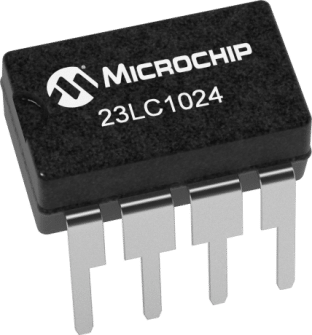
\includegraphics[width={0.2\textwidth}]{images/23lc1024}}
    \caption{SRAM Microchip 23LC1024 \cite{23lc1024}.}
    \label{fig:23LC1024}
\end{figure}

% There are ten SRAMs Microchip 23LC1024 that were available during the experiment. To check whether this SRAM is a justifiable candidate for PUF, several testings are performed.
% First, the number of 1's and 0's in memory after a start is calculated. Unfortunately, the average distribution of 1's and 0's are not similar, 1's occupy 70\% and 0's fill the remaining 30\%.
% Second, HD\textsubscript{intra} and HD\textsubscript{inter} are calculated on these chips. The calculation is done using twenty data of chip memory values on each chip which retrieved at room temperature, 5V input and 10 seconds interval between retrieval attempts. From these chips, the average HD\textsubscript{intra} is 6.18\% and the average HD\textsubscript{inter} is 42.54\%.
% Third, the effect of voltage variation on the HD\textsubscript{intra} and HD\textsubscript{inter} are also evaluated. The calculation is done using memory values on each chip which retrieved on room temperature and 10 seconds interval between retrieval attempts. The voltage range is between 2.5V and 5V with 0.5V increase on a step. On each step, there are three data retrieved. Using these data, voltage variation results in an average HD\textsubscript{intra} 8.21\% and an average HD\textsubscript{inter} 42.59\%.
%
% \begin{figure}[tph!]
%     \centerline{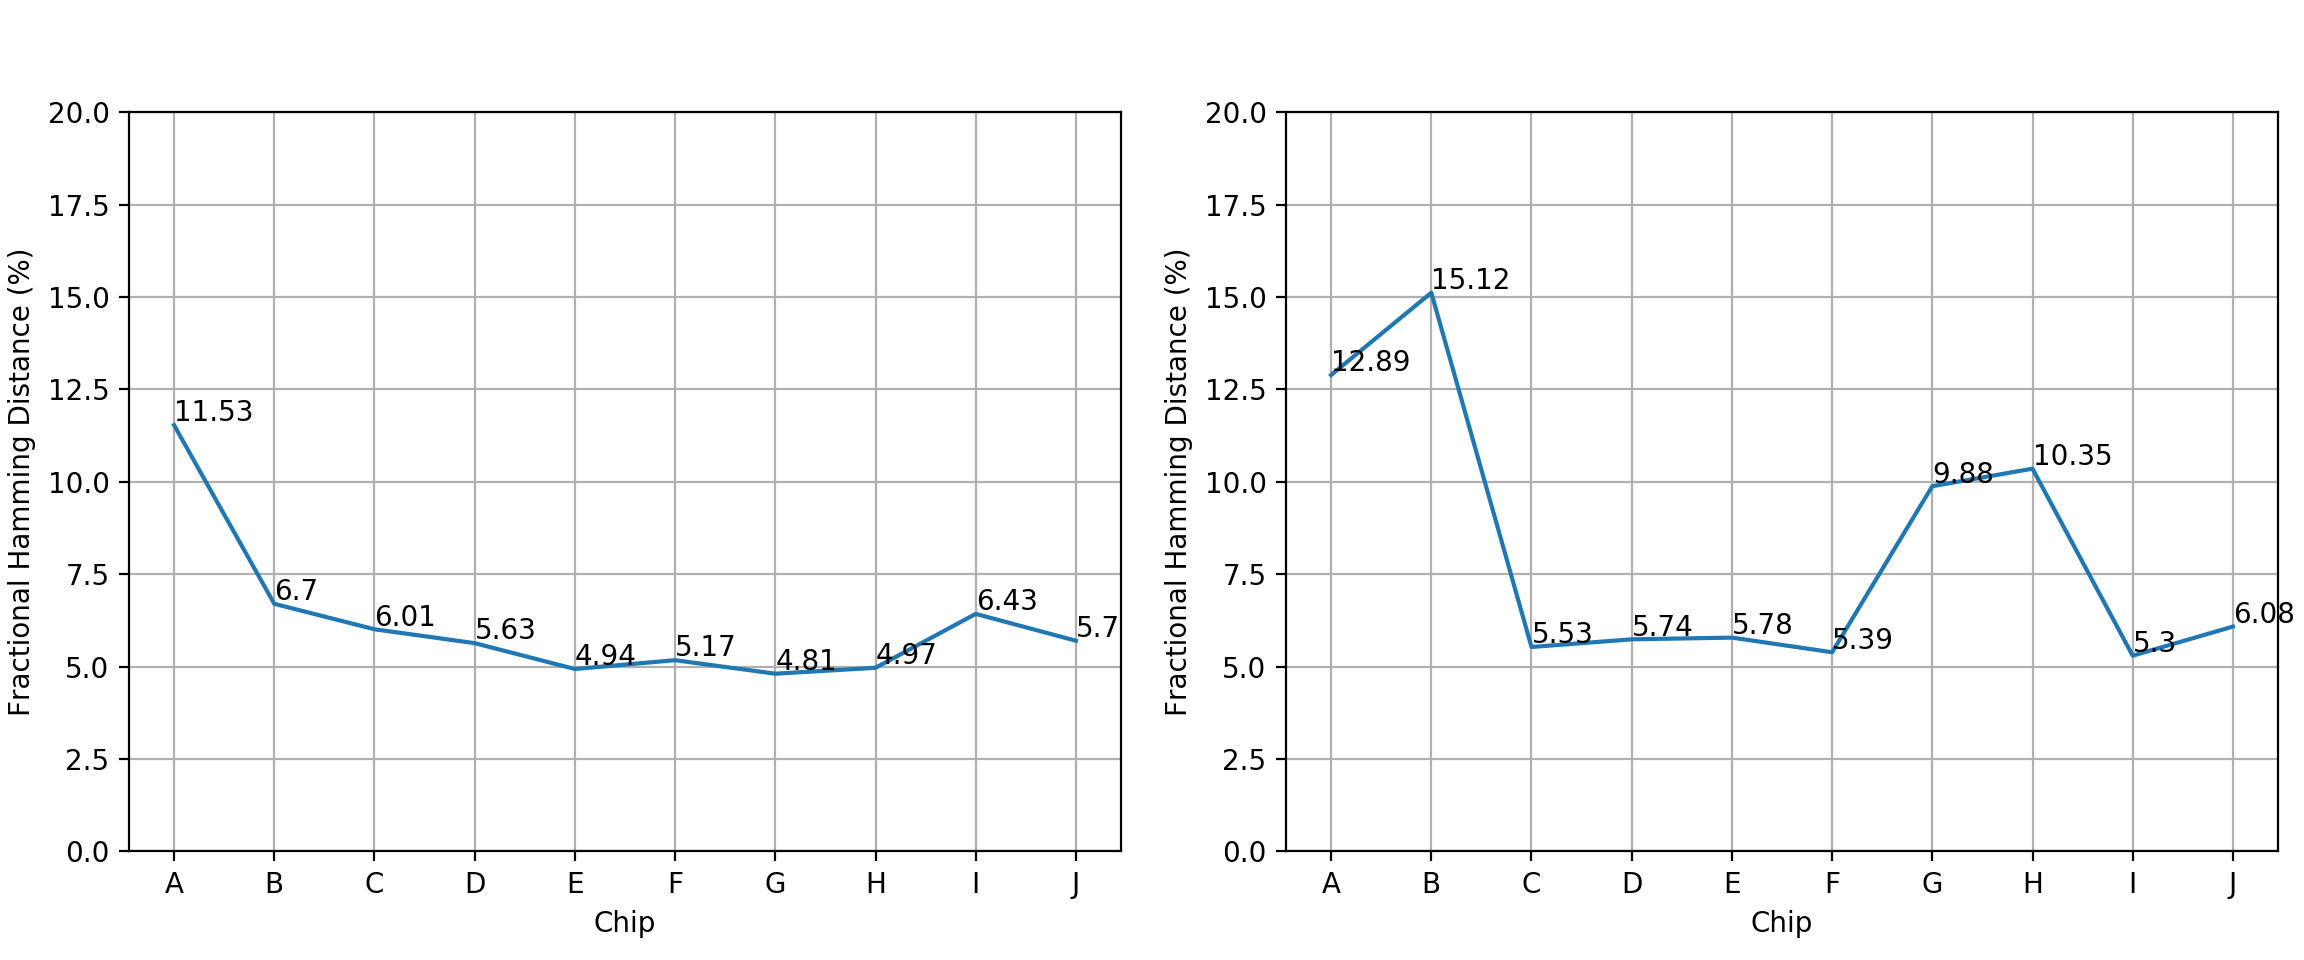
\includegraphics[width={\textwidth}]{images/23lc1024_hd_intra}}
%     \caption{HD\textsubscript{intra} of ten SRAMs Microchip 23LC1024. The left is HD\textsubscript{intra} with constant voltage, the right one is tested based on the voltage variation.}
%     \label{fig:23lc1024_hd_intra}
% \end{figure}
%
% Based on these experiments, SRAM Microchip 23LC1024 shows questionable results. First, the distribution of 1's and 0's inside the SRAM is not balanced. Second, a voltage variation shows that it significantly affects the  HD\textsubscript{intra}. Fortunately, there is no overlap between HD\textsubscript{intra} and HD\textsubscript{inter}. Even though these outcomes make us doubtful on this SRAM quality as an SRAM PUF candidate, we decided to continue using this SRAM in further experiments. Hopefully, when we locate the stable bits inside the SRAM, the experiments done on the stable bits will show a better result than this result.

\subsubsection{Cypress CY62256NLL}
The Cypress CY62256NLL is a 256 kbit SRAM device. Even though this device is less popular than Microchip 23LC1024, it is still widely used. One of the reason is that this device has an automatic power-down feature, reducing the power consumption by 99.9 percent when deselected. Unlike Microchip 23LC1024, Cypress CY62256NLL does not have an SPI connection which complicates the communication. To communicate, one should utilize its twenty-eight pins available. Since it has many pins, this contributes to its significantly larger size compared to Microchip 23LC1024. Specifically, its size is 37.592 × 13.97 × 4.953 mm and produced using 90nm technology. Its voltage range is ranging from 4.5V-5.5V. Figure \ref{fig:CY62256NLL} shows Cypress CY62256NLL.

\begin{figure}[tph!]
    \centerline{
\includegraphics[width={0.4\textwidth}]{images/cy62256nll}}
    \caption{SRAM Cypress CY62256NLL \cite{CY62256NLL}.}
    \label{fig:CY62256NLL}
\end{figure}

% There are five Cypress CY62256NLL SRAMs that were available during experiment. Similar like on previous SRAM, several testing are performed to check whether this SRAM is a justifiable candidate for PUF.
% First, the number of 1's and 0's in an initialization is counted. Fortunately, unlike the 23LC1024, the average distribution of 1's and 0's are similar, both occupy 50\% of total bits available.
% Next,
% HD\textsubscript{intra} and HD\textsubscript{inter} are calculated on both chips. The calculation is done using twenty data of chip memory values on each chip which retrieved at room temperature, 5V input and 10 seconds interval between retrieval attempts.
% From these chips, the average HD\textsubscript{intra} is 4.85\% and the average HD\textsubscript{inter} is 39.28\%.
% Last, the effect of voltage variation on the HD\textsubscript{intra} and HD\textsubscript{inter} are also evaluated. The calculation is done using chip memory values on each chip which retrieved on room temperature and 10 seconds interval between retrieval attempts. The voltage range is between 4.5V and 5V with 0.1V increase on each step. On each step, there are ten data enrolled.
% The average HD\textsubscript{inter} on voltage variation is 38.59\%, while HD\textsubscript{intra} is 3.58\%. Figure \ref{fig:cy62256nll_hd_intra} shows the HD\textsubscript{intra} between the constant and the variated voltage.
%
% \begin{figure}[tph!]
%     \centerline{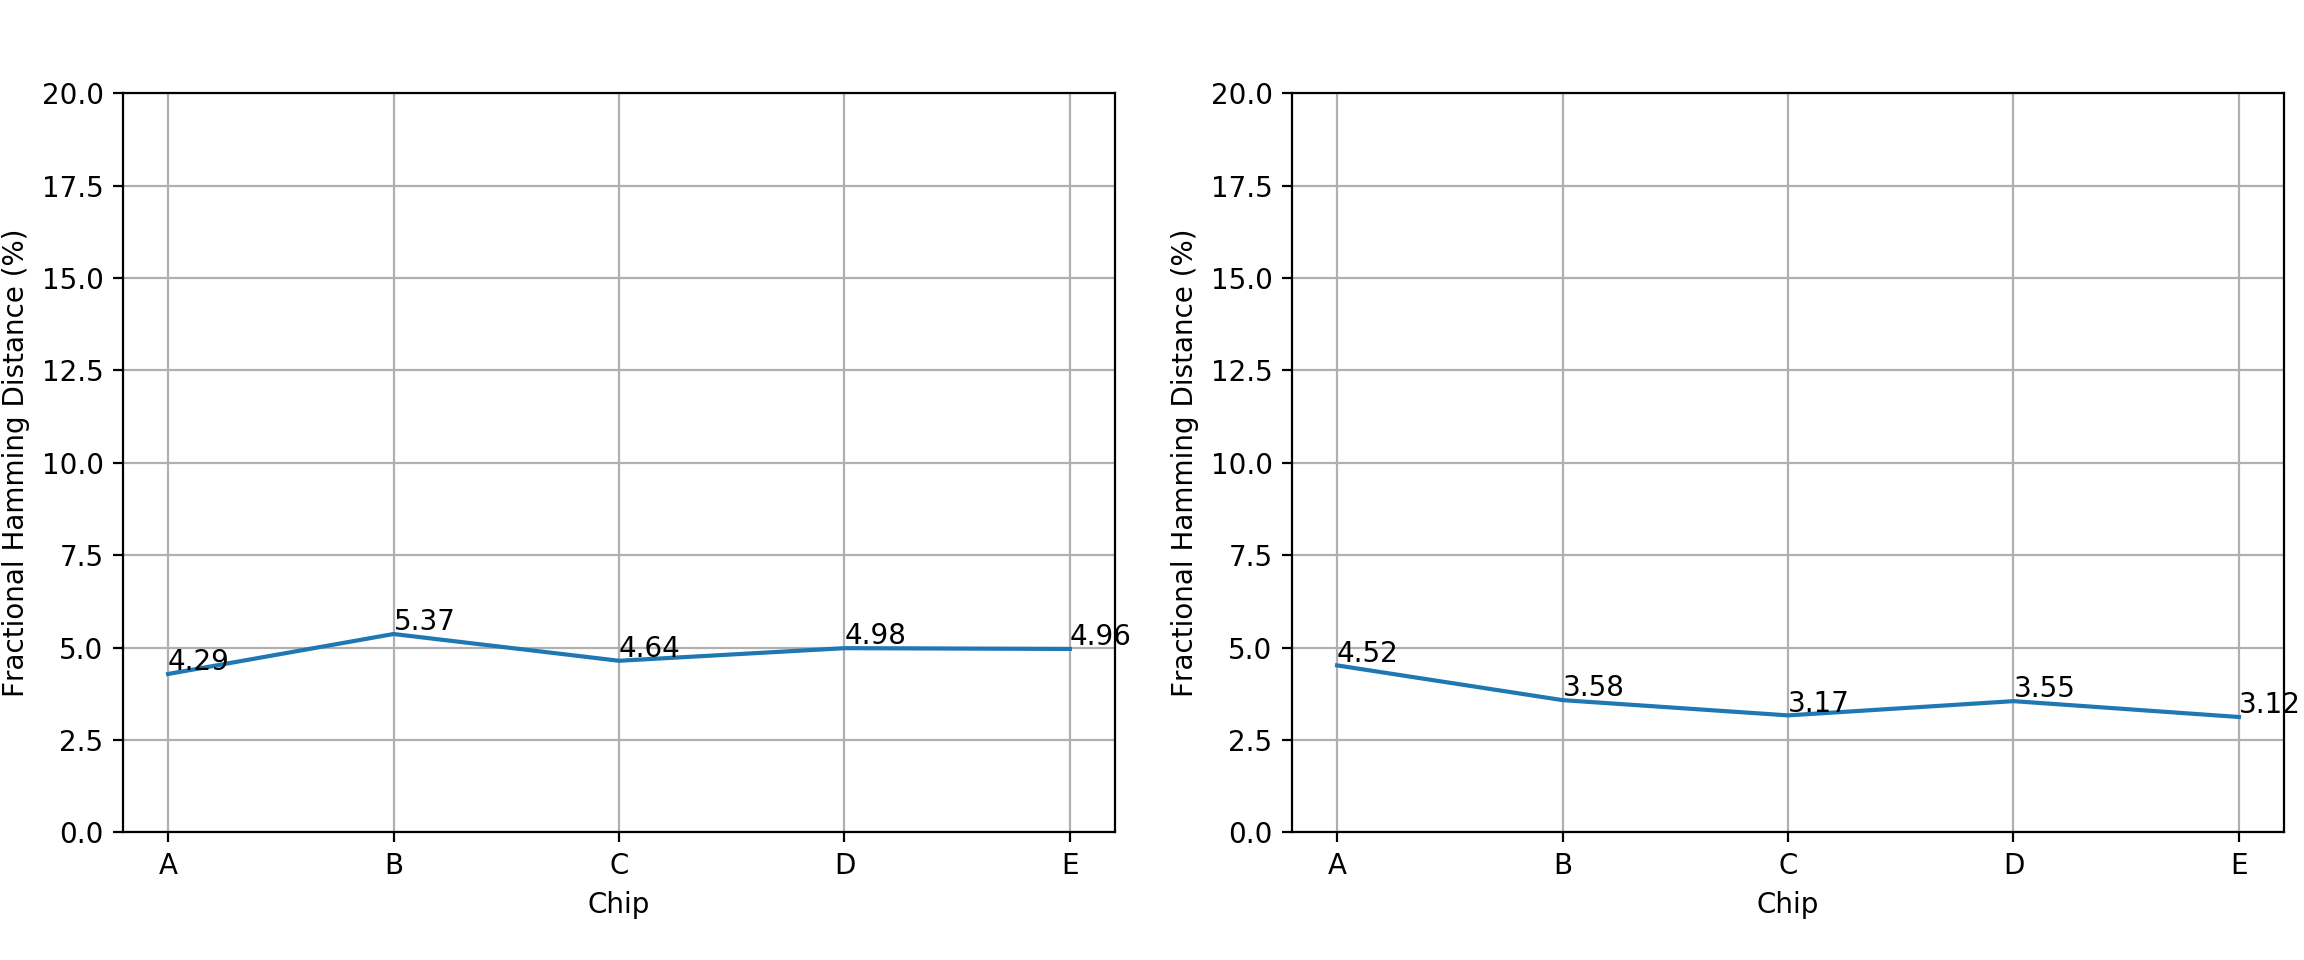
\includegraphics[width={\textwidth}]{images/cy62256nll_hd_intra}}
%     \caption{HD\textsubscript{intra} of five SRAMs Cypress CY62256NLL. The left is HD\textsubscript{intra} with constant voltage, the right one is tested based on the voltage variation.}
%     \label{fig:cy62256nll_hd_intra}
% \end{figure}
%
% The results shown above indicate that SRAM Cypress CY62256NLL is a qualified candidate for SRAM PUF. A well distributed 0's and 1's inside SRAM memory, voltage variation has little effect on HD\textsubscript{intra} and HD\textsubscript{inter}, and no overlap between HD\textsubscript{intra} and HD\textsubscript{inter} lead us to continue using this SRAM on further experiments.

\section{Automated PUF Profiling System}
To increase the experiment's efficiency, an automated PUF profiling system is constructed. The system consists of a PC, act as a master, and an Arduino connected to an external SRAM component which acts as a slave. A custom protocol was designed to communicate between them. It is specifically designed to be generic and usable for all types of PUF profiling measurements. The software on Arduino side waits for measurement commands sent by PC on the serial link after booting. The designed protocol is dedicated for read bytes, write bytes, and SRAM disable/enable. The system also supported parallel profiling which significantly increases the effectivity. Figure \ref{fig:puf_profiling} shows the setup and the schematic to profile four SRAMs Cypress CY62256NLL concurrently using four Arduino.

\begin{figure}[tph!]
    \centerline{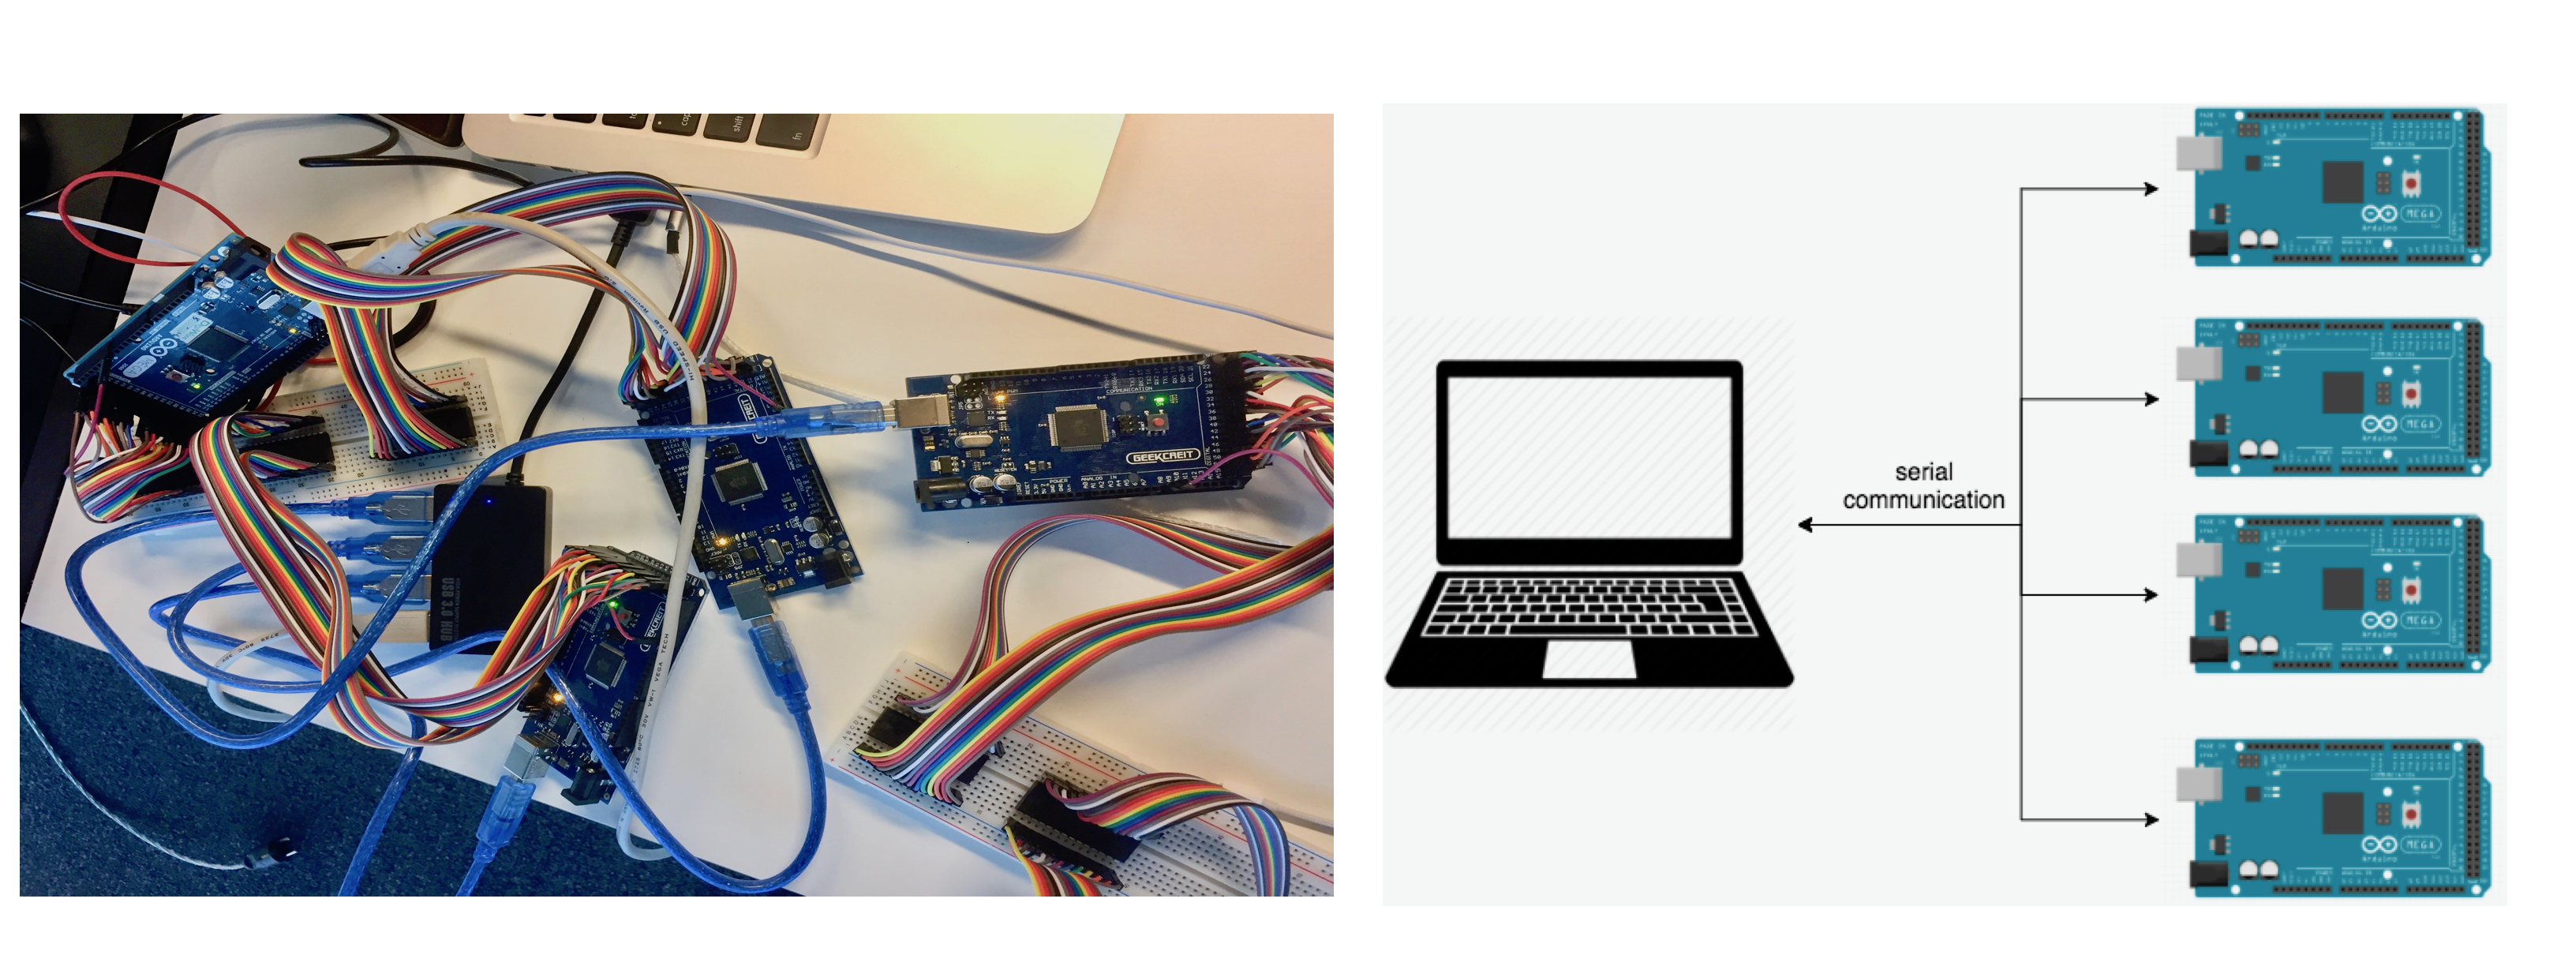
\includegraphics[width={\textwidth}]{images/setup}}
    \caption{Automated PUF profiling setup using a PC and four Arduino. Left picture shows the actual setup, while the right picture displays the schematic of such setup.}
    \label{fig:puf_profiling}
\end{figure}

\section{Testing on Chosen Off-The-Shelf SRAMs}

As mentioned in Chapter 2, to be qualified as a PUF candidate, an SRAM has to be stable in various conditions. This means if it is given various power input or used in varied temperatures or utilized for a long time, the initialized SRAM values has to remain similar or only has little changes (HD\textsubscript{intra} has to be lower than the maximum error correction capability of the key generation scheme mentioned in Section \ref{ch:key_generation_scheme}, 12.7\%). Under any condition, there should be no overlap between HD\textsubscript{intra} and HD\textsubscript{inter}. Moreover, the SRAM has to have a sufficient amount of randomness, shown by having equal distributions between 1's and 0's on its values.  To ensure the quality of these two SRAMs, there are several experiments performed on each SRAM, such as calculating HD\textsubscript{intra} and HD\textsubscript{inter} given the whole memory value as the challenge and also the distribution of 1's and 0's inside SRAM memory.

\subsubsection{Microchip 23LC1024}
There are ten SRAMs Microchip 23LC1024 that were available during the experiment. To check whether this SRAM is a justifiable candidate for PUF, several testings are performed.
First, the number of 1's and 0's in memory after a start is calculated. Unfortunately, the average distribution of 1's and 0's are not similar, 1's occupy 70\% and 0's fill the remaining 30\%.
Second, HD\textsubscript{intra} and HD\textsubscript{inter} are calculated on these chips. The calculation is done using twenty memory values on each chip which retrieved at room temperature, 5V input and 10 seconds interval between retrieval attempts. From these chips, the average HD\textsubscript{intra} is 6.18\% and the average HD\textsubscript{inter} is 42.54\%.
Third, the effect of voltage variation on the HD\textsubscript{intra} and HD\textsubscript{inter} are also evaluated. The calculation is done using memory values on each chip which retrieved on room temperature and 10 seconds interval between retrieval attempts. The voltage range is between 2.5V and 5V with 0.5V increase on a step. On each step, there are three data retrieved. Using these data, voltage variation results in an average HD\textsubscript{intra} 8.21\% and an average HD\textsubscript{inter} 42.59\%.

\begin{figure}[tph!]
    \centerline{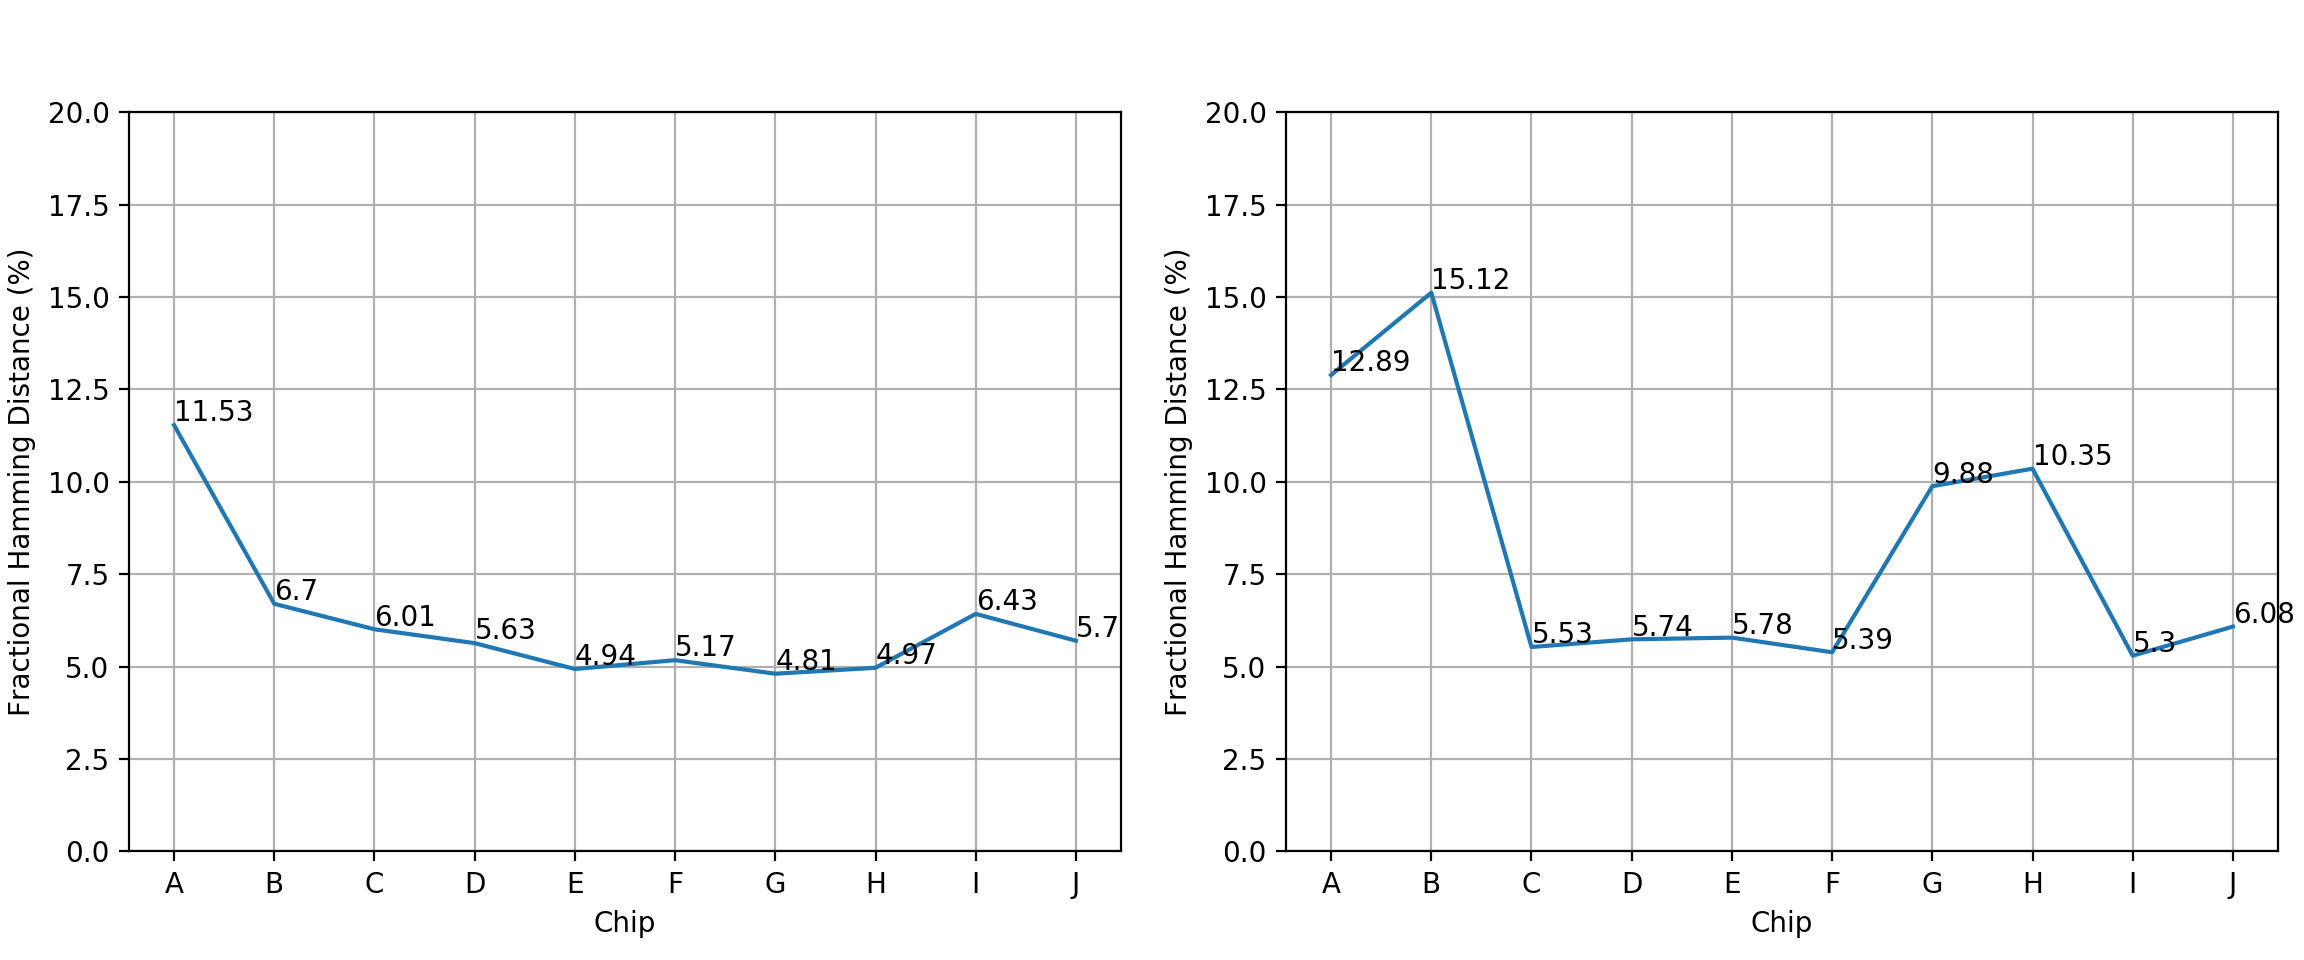
\includegraphics[width={\textwidth}]{images/23lc1024_hd_intra}}
    \caption{HD\textsubscript{intra} of ten SRAMs Microchip 23LC1024. The left figure is the testing result of HD\textsubscript{intra} with constant voltage, the right one is tested based on the voltage variation.}
    \label{fig:23lc1024_hd_intra}
\end{figure}

Based on these experiments, SRAM Microchip 23LC1024 shows questionable results. First, the distribution of 1's and 0's inside the SRAM is not balanced. Second, a voltage variation shows that it significantly affects the  HD\textsubscript{intra}. Third, there are two SRAMs Microchip 23LC1024 ('A' and 'B') that shows HD\textsubscript{intra} larger than the maximum error correction capability of the key generation scheme (12.7\%) when they are tested on the effect of voltage variation. Fortunately, there is no overlap between HD\textsubscript{intra} and HD\textsubscript{inter}. Even though these outcomes make us doubtful on this SRAM quality as an SRAM PUF candidate, we decided to continue using this SRAM in further experiments. Hopefully, when we locate the stable bits inside the SRAM, the experiments done on the stable bits will show a better result than this result.

\subsubsection{Cypress CY62256NLL}

There are five SRAMs Cypress CY62256NLL that were available during experiment. Similar like on previous SRAM, several testing are performed to check whether this SRAM type is a justifiable candidate for PUF.
First, the number of 1's and 0's in an initialization is counted. Fortunately, unlike the 23LC1024, the average distribution of 1's and 0's are similar, both occupy 50\% of total bits available.
Next,
HD\textsubscript{intra} and HD\textsubscript{inter} are calculated on both chips. The calculation is done using twenty memory values on each chip which retrieved at room temperature, 5V input and 10 seconds interval between retrieval attempts.
From these chips, the average HD\textsubscript{intra} is 4.85\% and the average HD\textsubscript{inter} is 39.28\%.
Last, the effect of voltage variation on the HD\textsubscript{intra} and HD\textsubscript{inter} are also evaluated. The calculation is done using chip memory values on each chip which retrieved on room temperature and 10 seconds interval between retrieval attempts. The voltage range is between 4.5V and 5V with 0.1V increase on each step. On each step, there are ten data enrolled.
The average HD\textsubscript{inter} on voltage variation is 38.59\%, while HD\textsubscript{intra} is 3.58\%. Figure \ref{fig:cy62256nll_hd_intra} shows the HD\textsubscript{intra} between the constant and the variated voltage.

\begin{figure}[tph!]
    \centerline{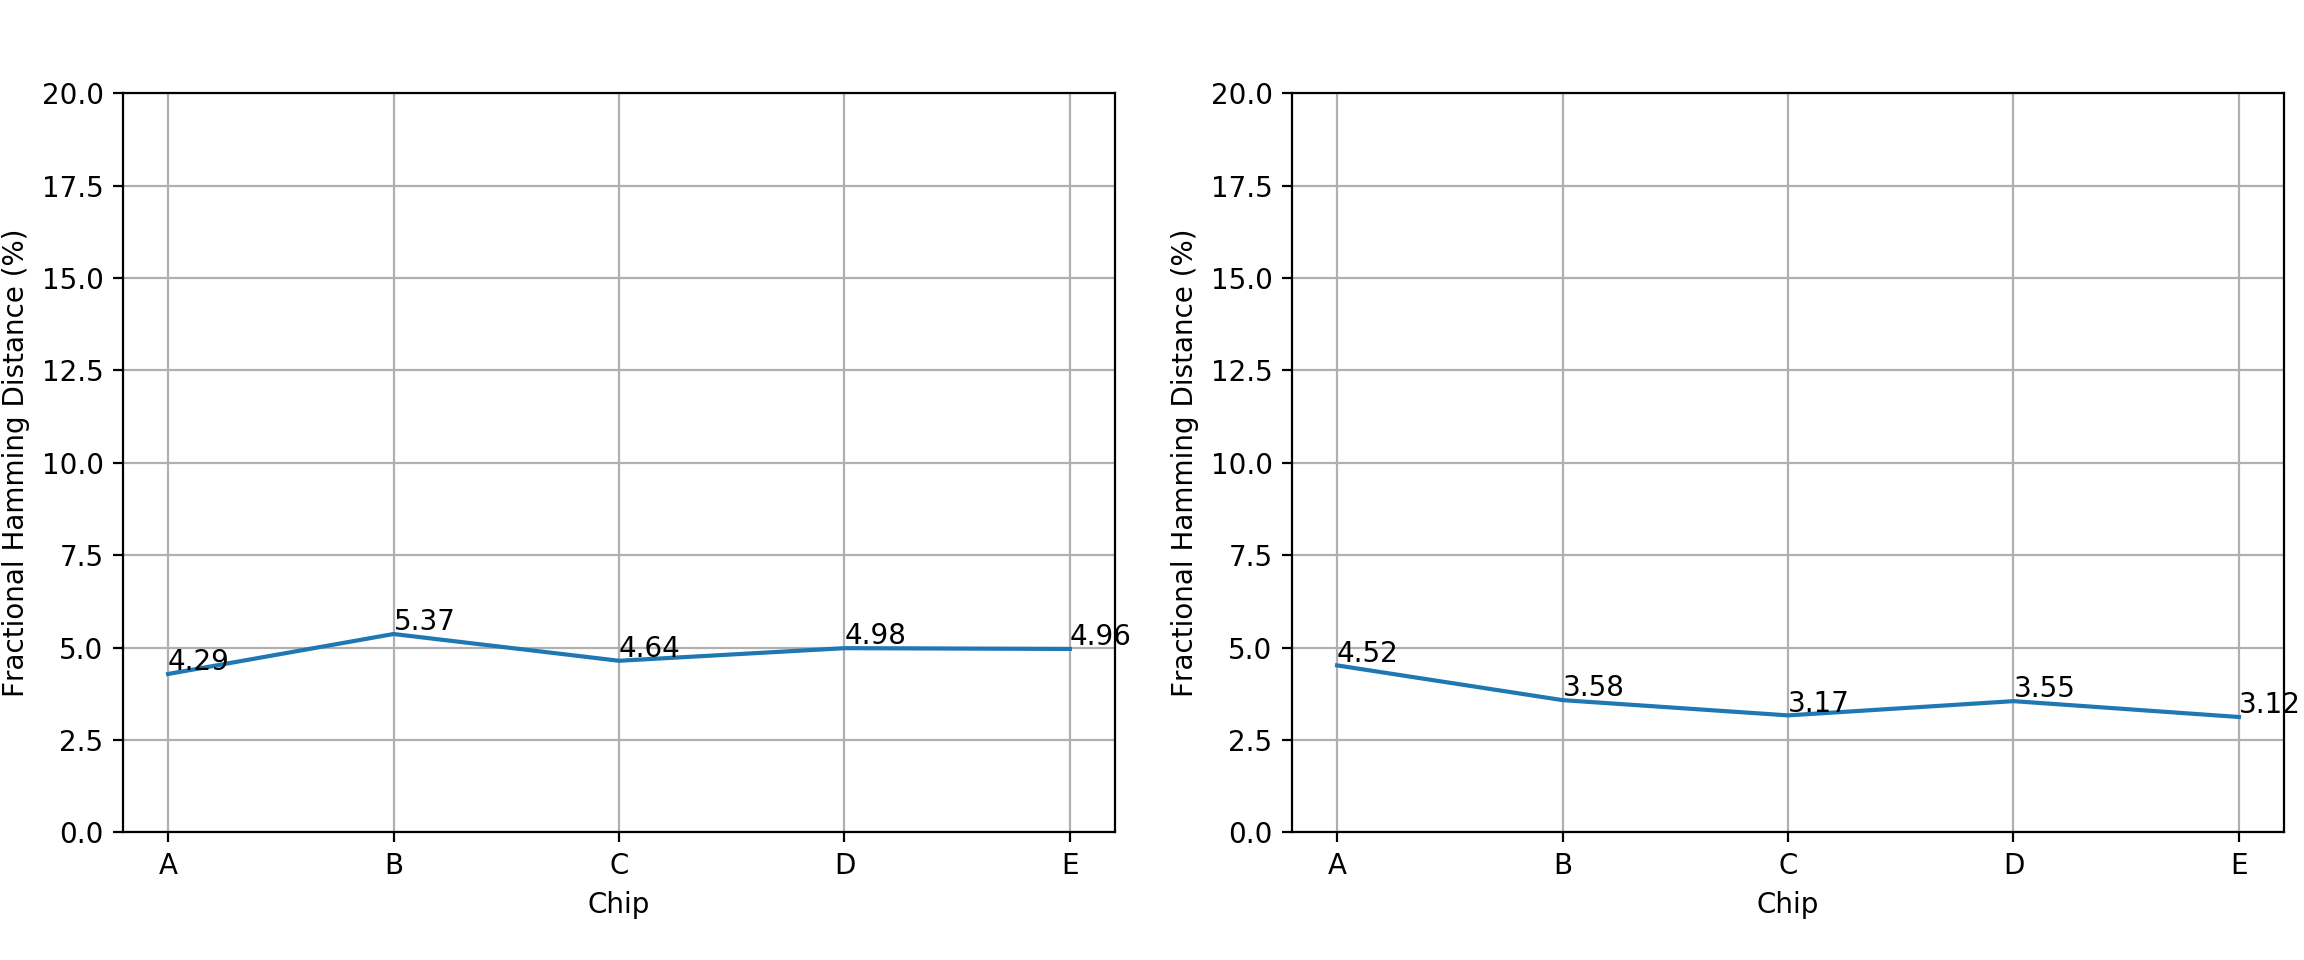
\includegraphics[width={\textwidth}]{images/cy62256nll_hd_intra}}
    \caption{HD\textsubscript{intra} of five SRAMs Cypress CY62256NLL. The left figure is the testing result of HD\textsubscript{intra} with constant voltage, the right one is tested based on the voltage variation.}
    \label{fig:cy62256nll_hd_intra}
\end{figure}

The results shown above indicate that SRAM Cypress CY62256NLL is a qualified candidate for SRAM PUF. A well distributed 0's and 1's inside SRAM memory, voltage variation has little effect on HD\textsubscript{intra} and HD\textsubscript{inter}, and no overlap between HD\textsubscript{intra} and HD\textsubscript{inter} lead us to continue using this SRAM for further experiments.

\section{Testing on Bit Selection Algorithms}

In this section, the test on stable bits produced by two algorithms, neighbor stability and data remanence analysis, is shown. The test was done on a single chip of each SRAM type.
% , one 23L1024 and one CY62256NLL.
The explanation of both algorithms can be found on Section \ref{lbl:bit-selection}.

\subsection{Neighbour Stability Analysis}
To use this algorithm, first, data of SRAM bits value from various conditions (voltages and time difference between data retrieval attempts) need to be gathered. Afterwards, the bits which remained stable over all retrieved data are located. Then, the rank of remained stable bits are calculated. Last, n bits with highest rank can be used according to the necessity. The higher the rank, the more stable that bit should be.

\subsubsection{Microchip 23LC1024}
As input for the algorithm, there are 500 data of SRAM bits value used for this chip. The voltage variation is randomized between 2.5V - 5.0V. The time difference between data retrieval attempts is ranging from 5 seconds until 1 hour.
SRAM Microchip 23LC1024 itself has capacity 1048576 bits. After doing the calculation from those five hundred data, there are 413374 remaining stable bits. From those remaining stable bits, the rank of each bit is calculated. The frequency of bits rank is shown in Figure \ref{fig:23lc1024_score_rank_bits}. As shown in this figure, the total bits with rank more than 5 is insignificant, only showing 493 bits. Bits with rank more or equal to six is merged into a single bar because the frequency among those rank is usually only a single digit.

\begin{figure}[tph!]
    \centerline{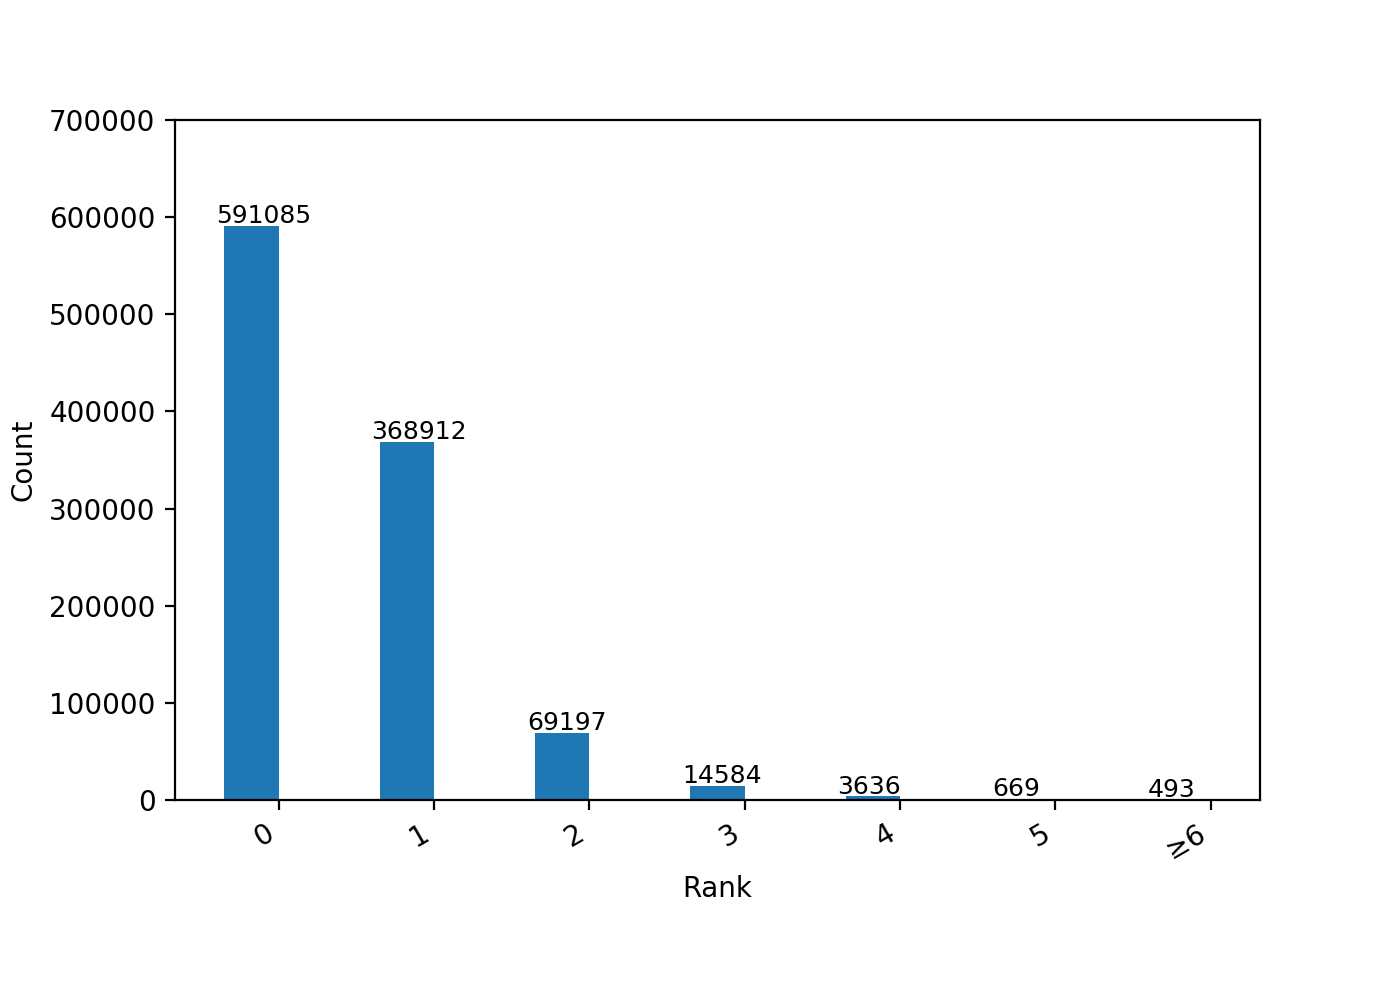
\includegraphics[width={0.9\textwidth}]{images/23lc1024_score_rank_bits}}
    \caption{Remaining stable bits count according to their rank in SRAM Microchip 23LC1024.}
    \label{fig:23lc1024_score_rank_bits}
\end{figure}

\subsubsection{Cypress CY62256NLL}
Similar like with SRAM Microchip 23LC1024, there are 500 memory values retrieved in SRAM Cypress CY62256NLL.
Cypress CY62256NLL is able to store 262144 bits in its memory. The remained stable bits after 500 data retrieval are 102708 bits (39,18\%).
The result of the calculation is shown on Figure \ref{fig:cy62256nll_score_rank_bits}. Compared to Microchip 23LC1024, this SRAM shows more promising result since there are many bits with ranks more than seven. Even to get two thousand stable bits, the lowest rank that can be included is twelve.

\begin{figure}[tph!]
    \centerline{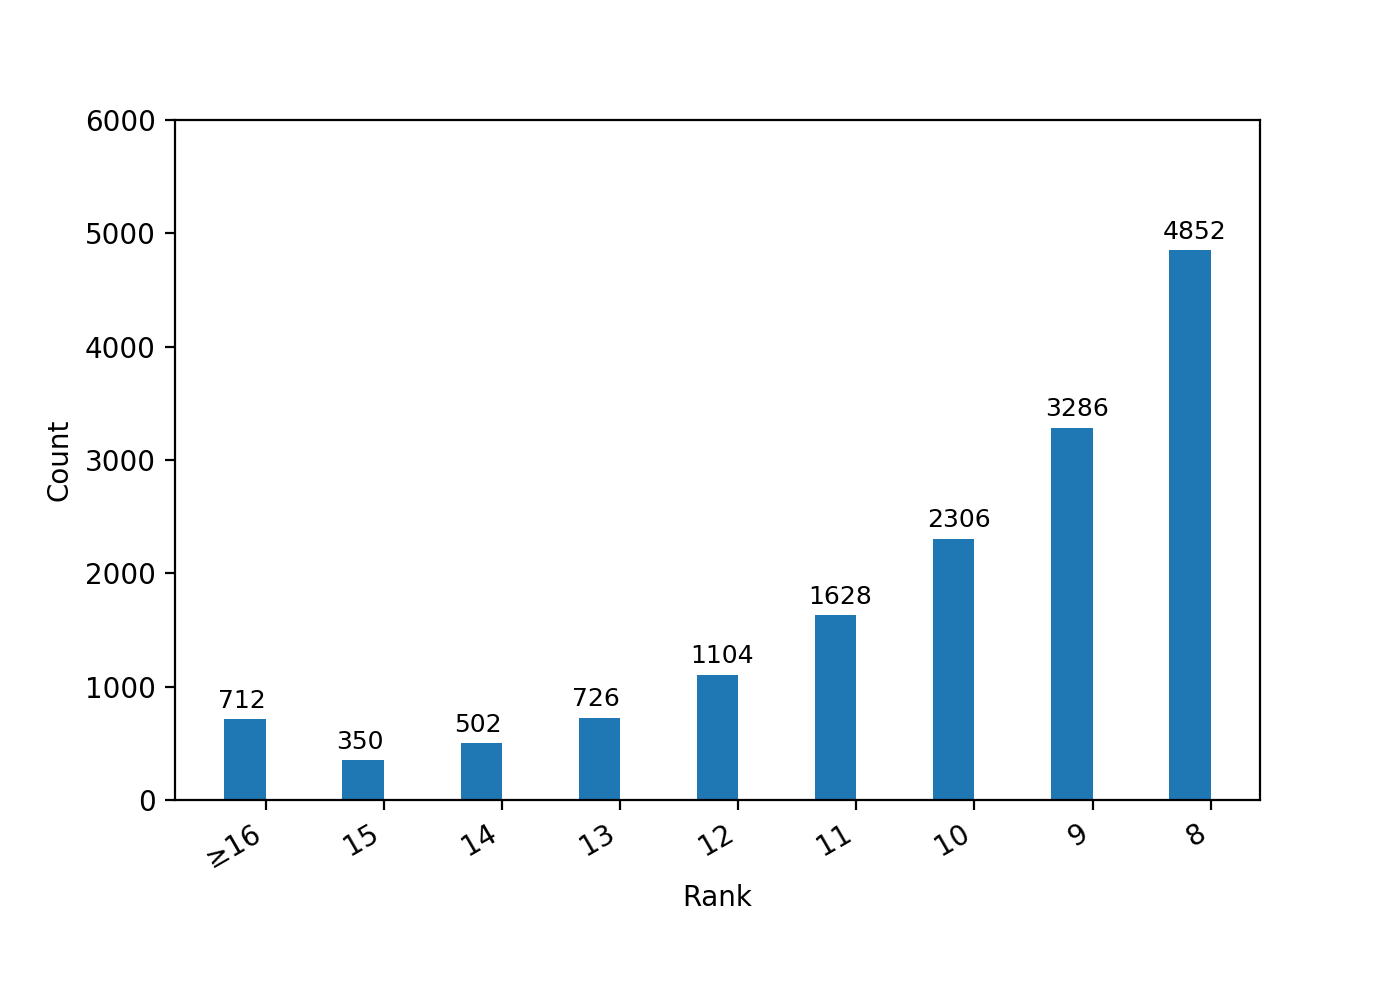
\includegraphics[width={0.9\textwidth}]{images/cy62256nll_score_rank_bits}}
    \caption{Remaining stable bits count according to their rank in SRAM Cypress CY62256NLL. There are 246678 bits with rank less or equal to seven.}
    \label{fig:cy62256nll_score_rank_bits}
\end{figure}

% \pagebreak
\subsection{Data Remanence Approach}

The result of data remanence analysis on both SRAMs is shown below.

\subsubsection{Microchip 23LC1024}

On SRAM Microchip 23LC1024, the data remanence analysis is done on time variance between 0-1.0 second. The result can be seen on Figure \ref{fig:23lc1024-remanence0}. In this figure, it is shown that
SRAM Microchip 23LC1024 will reach the uninitialized point if it is temporarily turn off for 0.7 seconds.

\begin{figure}[tph!]
    \centerline{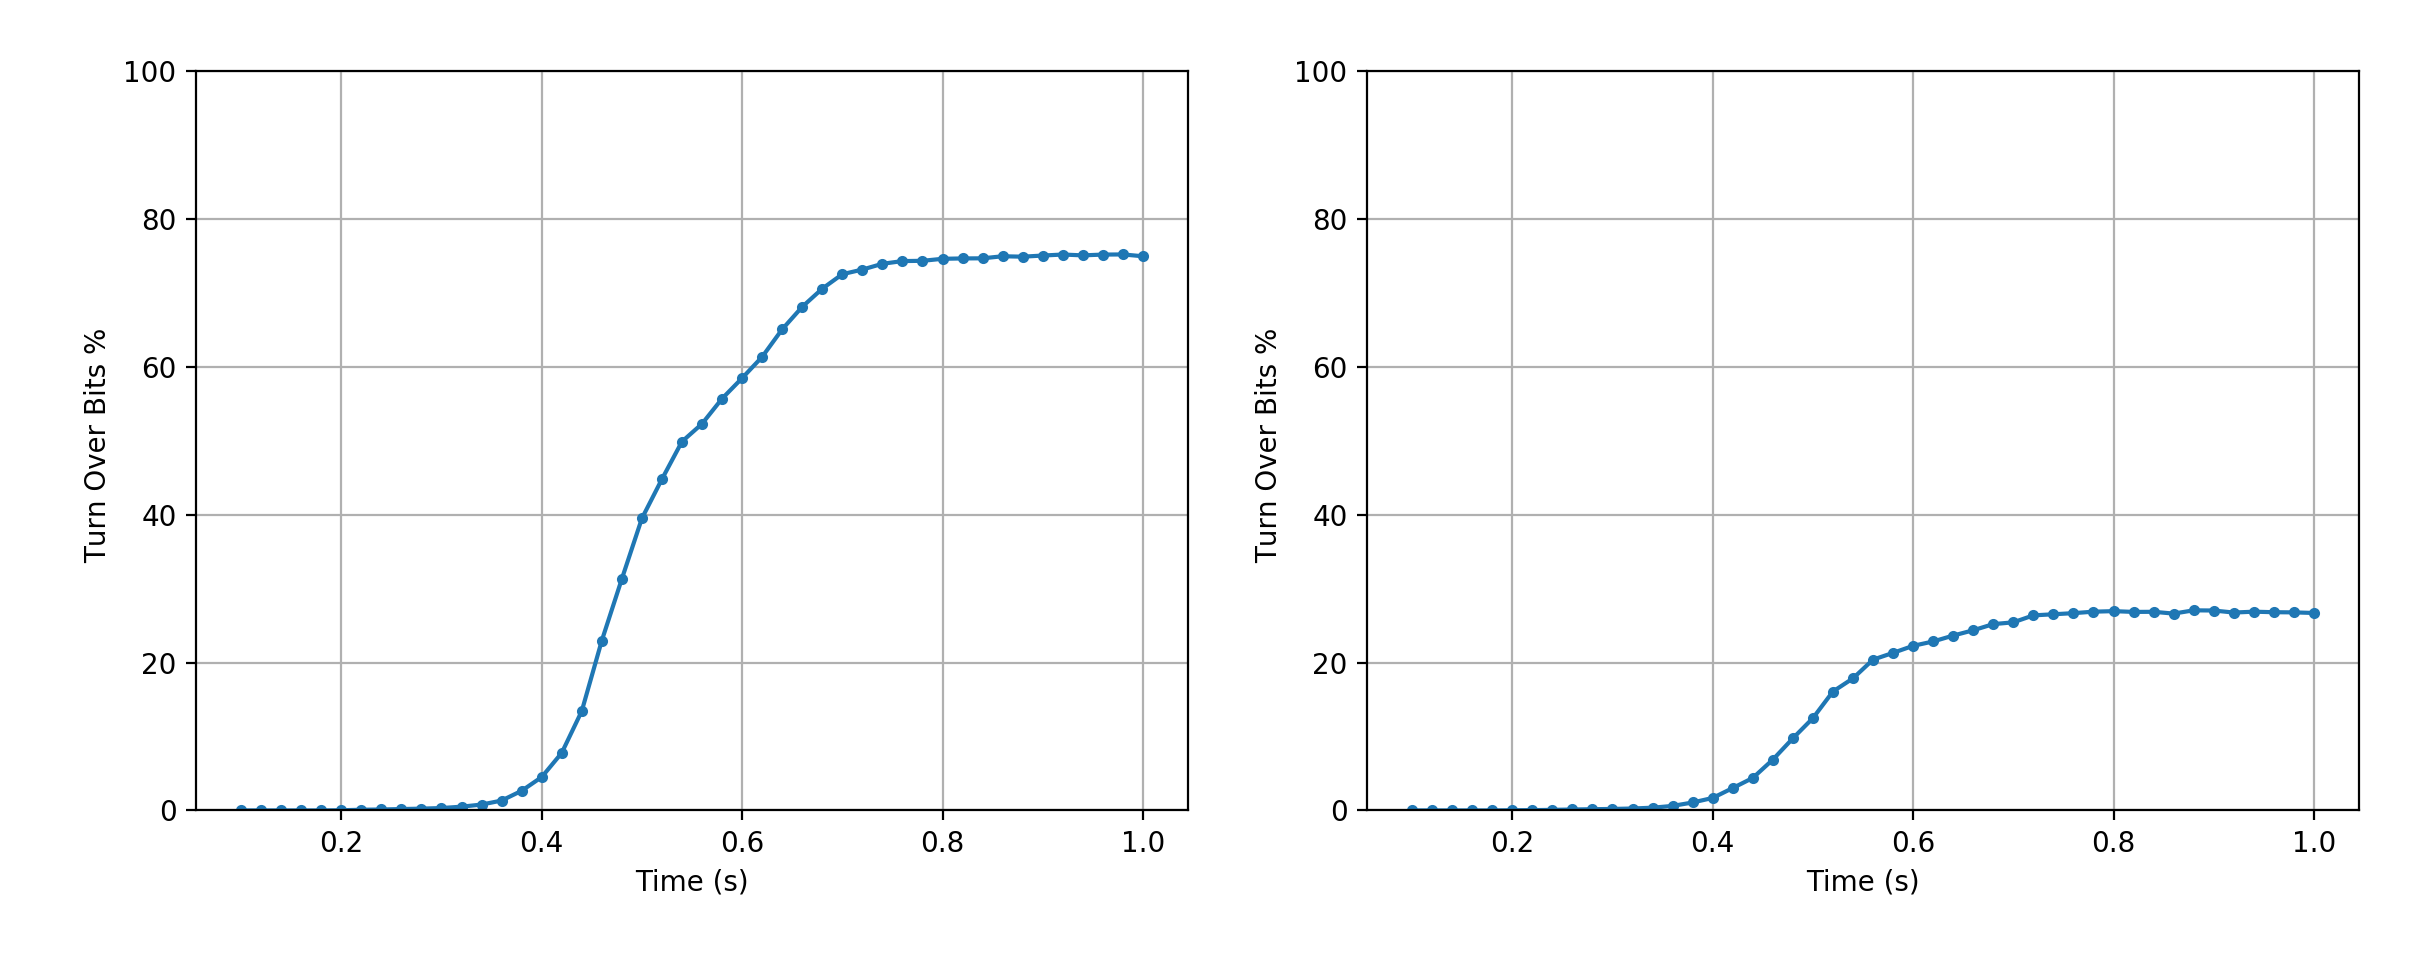
\includegraphics[width={\textwidth}]{images/remanence_23lc1024}}
    \caption{Measured SRAM Microchip 23LC1024 data remanence for data 0 (left) and data 1 (right).
    % Remanence Graph of SRAM Microchip 23LC1024. Left is remanence 0 and right is remanence 1.
    SRAM Microchip 23LC1024 will reach the uninitialized point if it is temporarily shut down for 0.7 second.}
    \label{fig:23lc1024-remanence0}
\end{figure}



\subsubsection{Cypress CY62256NLL}

On SRAM Cypress CY62256NLL, the data remanence analysis is done on time variance between 0-10 seconds. The result can be seen on Figure \ref{fig:23lc1024-remanence0}. In this figure, it is shown that
SRAM Cypress CY62256NLL will reach the uninitialized point if it is temporarily shut down for 5.0 second.

\begin{figure}[tph!]
    \centerline{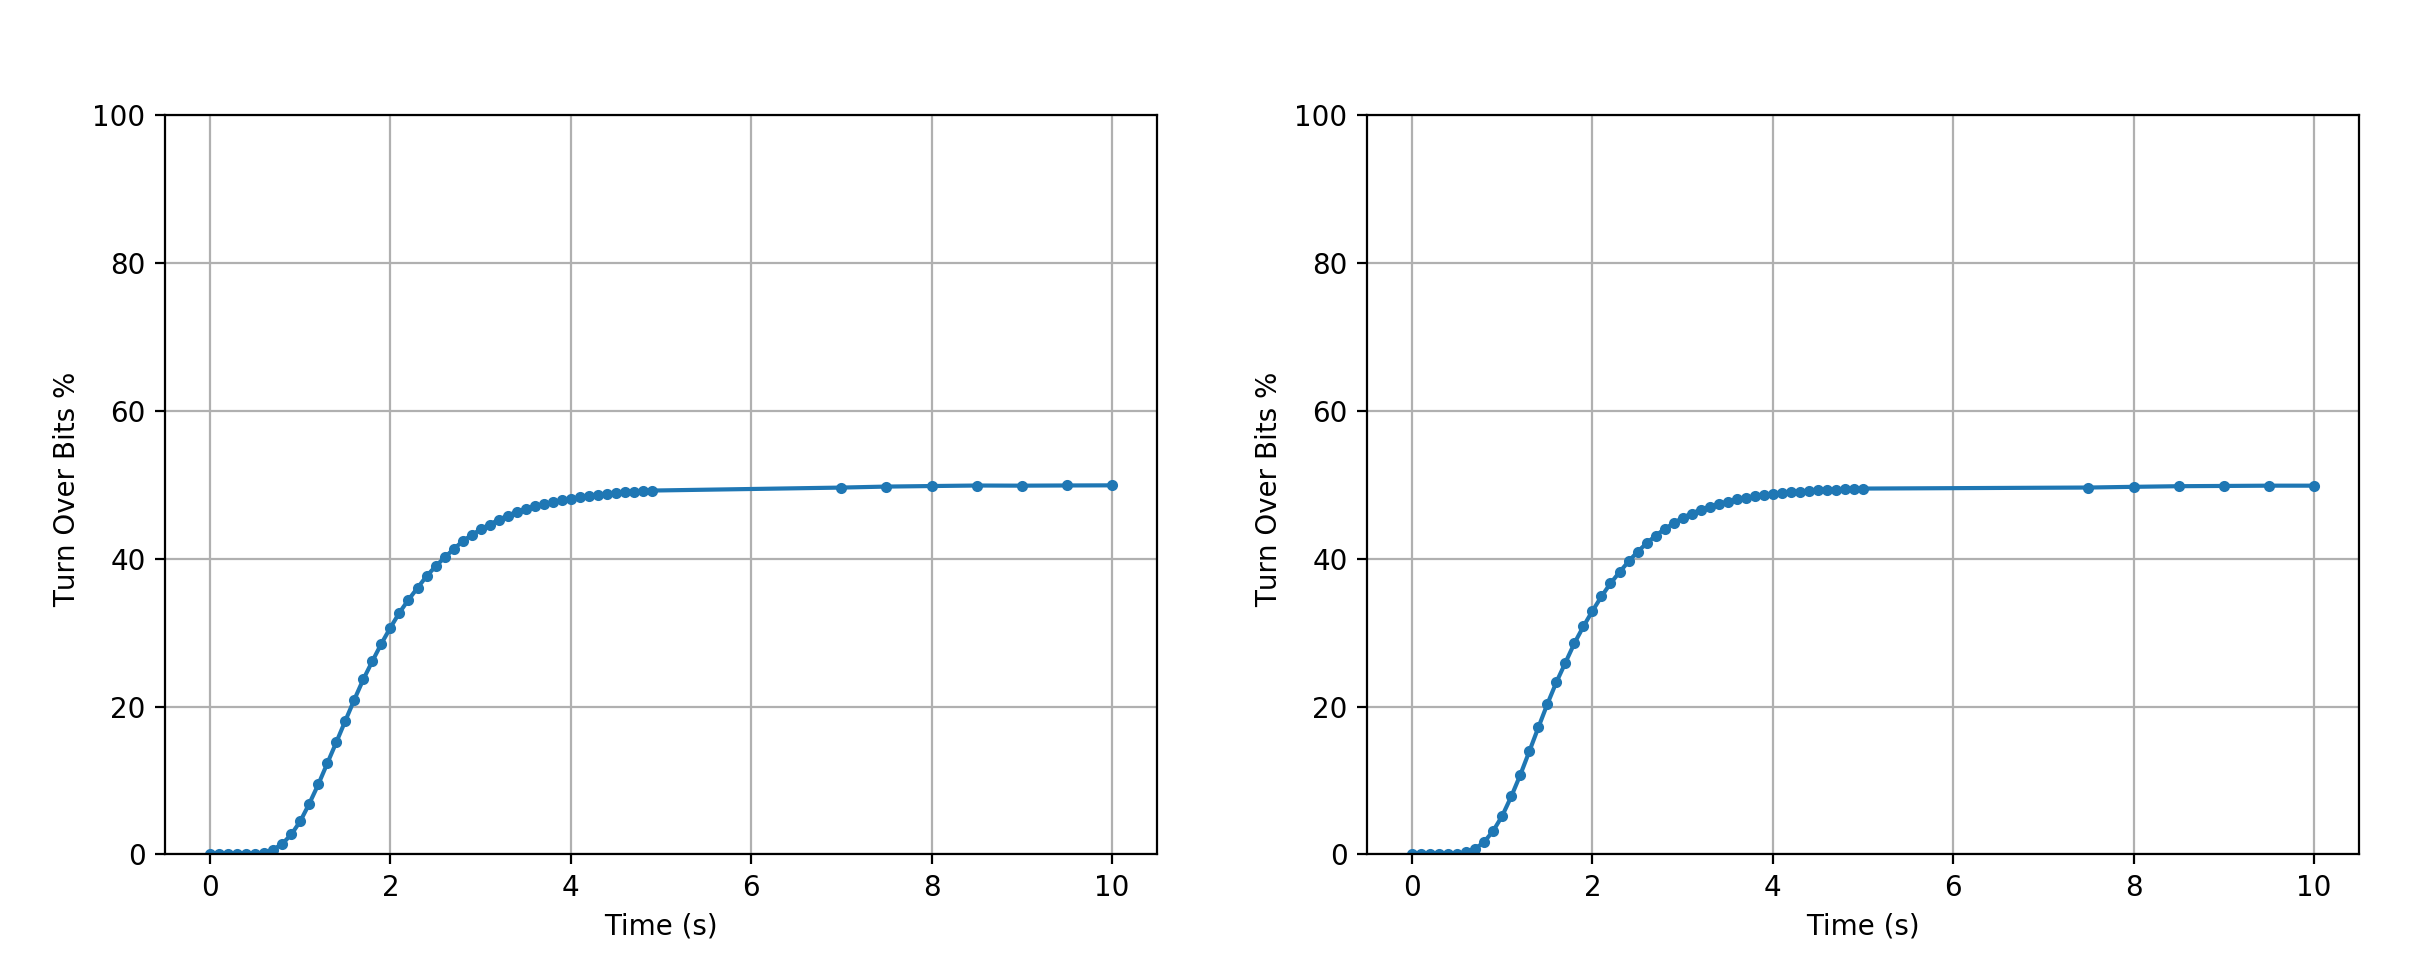
\includegraphics[width={\textwidth}]{images/remanence_cy62256nll}}
    \caption{Measured SRAM Cypress CY62256NLL data remanence for data 0 (left) and data 1 (right).
    % Remanence Graph of CY62256NLL. Left is remanence 0 and right is remanence 1.
    SRAM Cypress CY62256NLL will reach the uninitialized point if it is temporarily shut down for 5.0 second.}
    \label{fig:CY62256NLL-remanence0}
\end{figure}


\subsection{Stability Test on Stable Bits}\label{ch:hd_intra_stable}
In this section, test results on the effect of time interval and voltage on stable bits using both algorithms on each SRAM are shown. The effect of aging and temperature is not tested due to a limitation on time and equipment. For the effect of time interval testing, the enrollment was done on 16 days with one day gap between enrollment. Voltage effect testing was done on voltage ranging from 4.5V-5V for SRAM Cypress CY62256NLL and 2.5V-5V for SRAM Microchip 23LC1024. The test is done on 4662 bits which is twice the length of the bits required to generate 256 bits key when using scheme shown in Figure \ref{fig:key-generation-scheme}. The result of time interval testing on SRAM Microchip 23LC1024 is shown on Figure \ref{fig:test_stable_23lc1024}, while Figure \ref{fig:test_stable_cy62256nll} displays the result for SRAM Cypress CY62256NLL.

\begin{figure}[tph!]
    \centerline{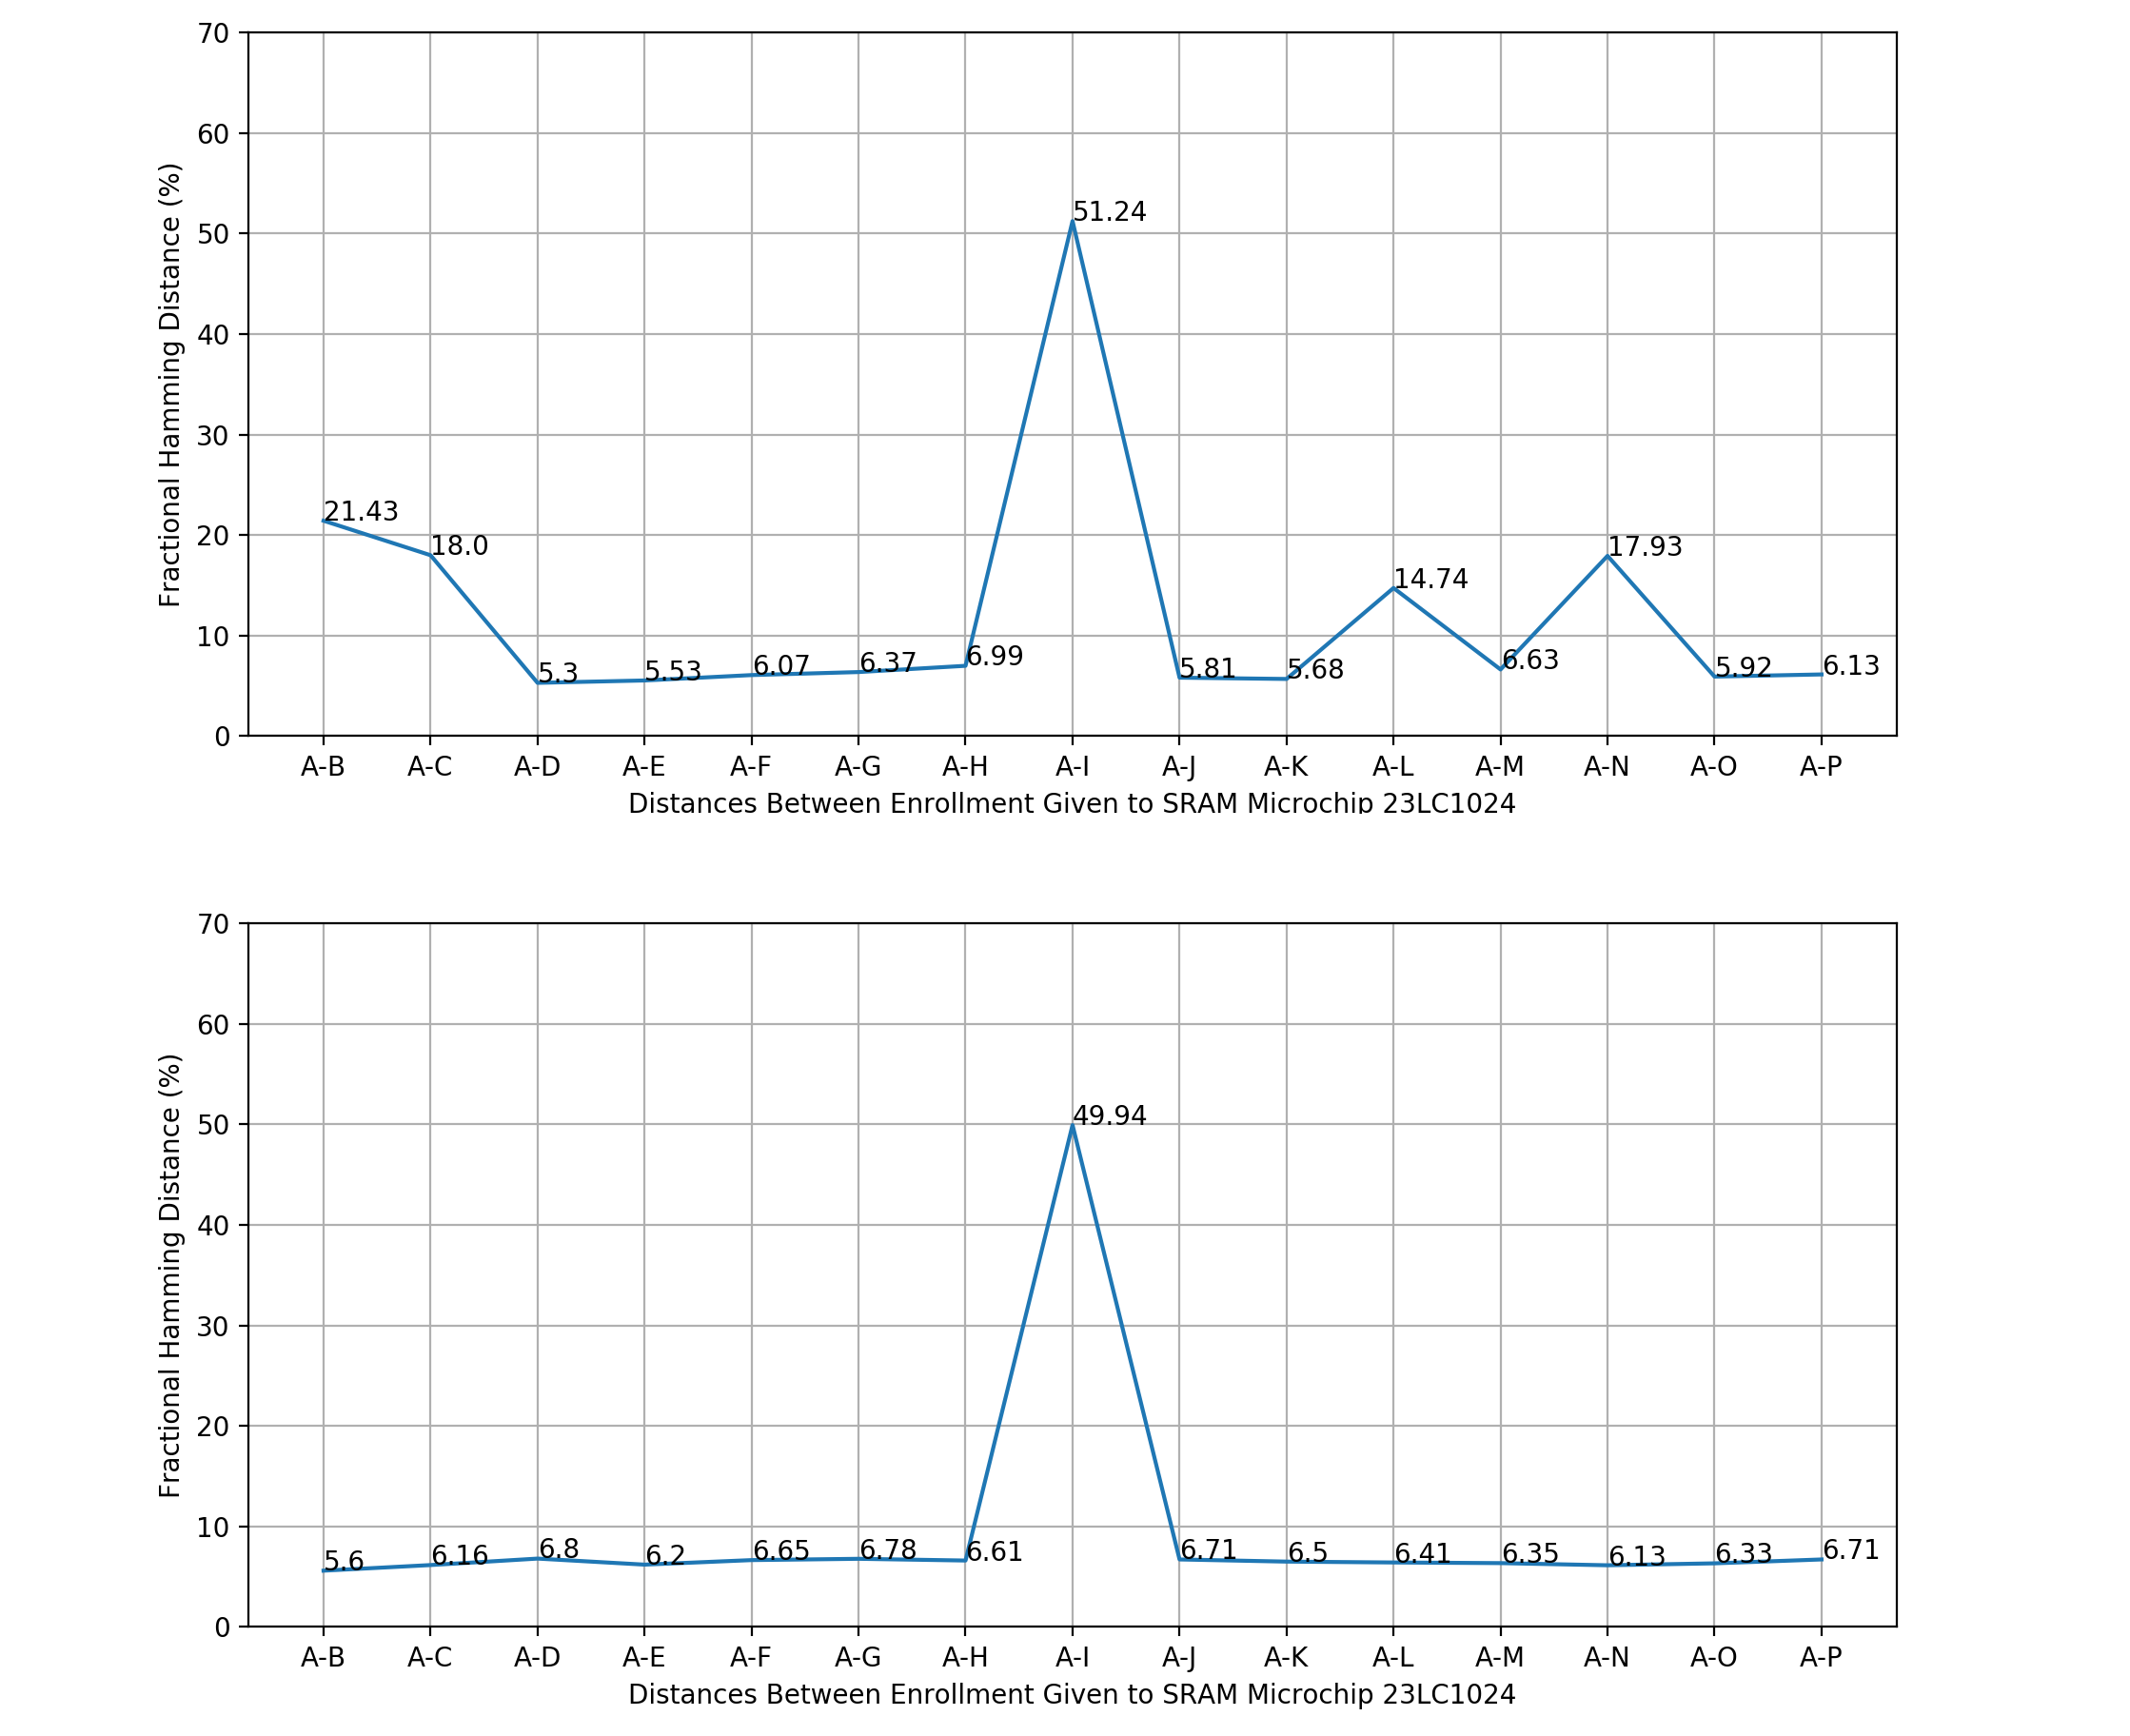
\includegraphics[width={1.1\textwidth}]{images/23lc1024_hd_intra_time_stable}}
    \caption{Time interval testing results on SRAM Microchip 23LC1024. The top figure is the testing result on stable bits generated using neighbor analysis, while the bottom one is tested on stable bits generated using data remanence approach. Index A on x-axis refers to enrollment on day 1, B on day 2, etc. Index A-B refers to fractional hamming distance between enrollment on day 1 and day 2.}
    \label{fig:test_stable_23lc1024}
\end{figure}

\begin{figure}[tph!]
    \centerline{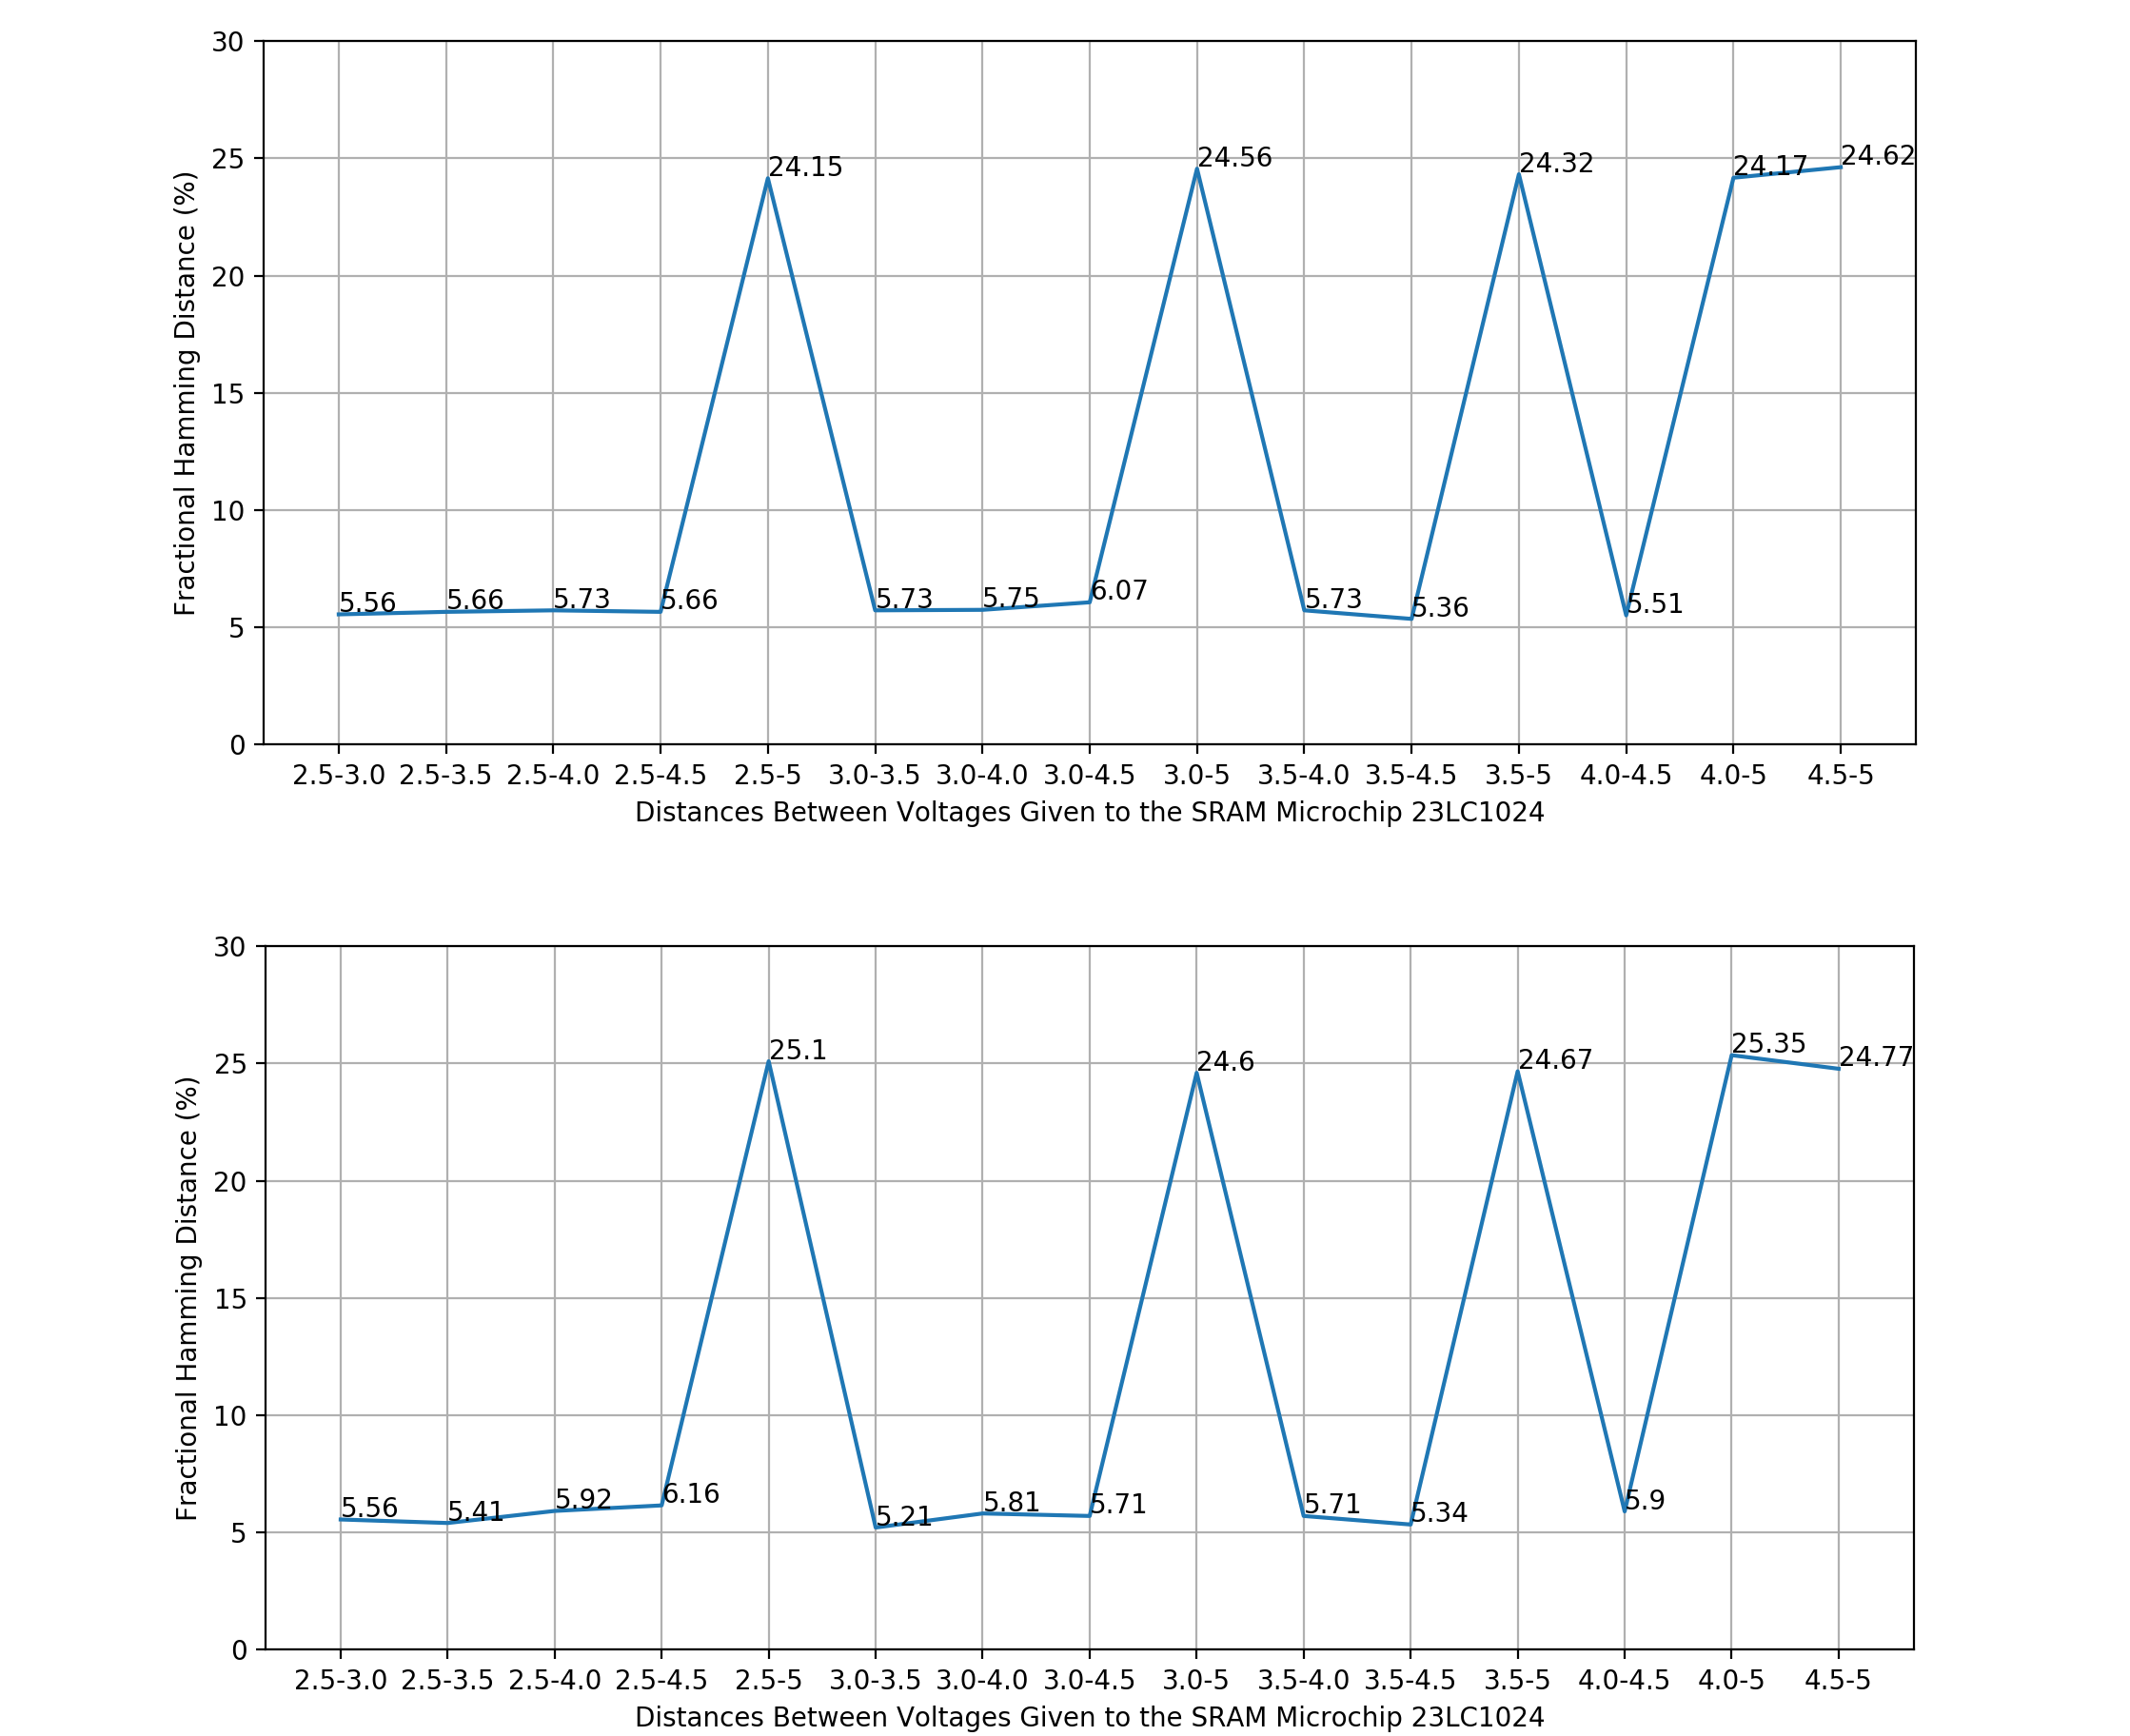
\includegraphics[width={1.1\textwidth}]{images/23lc1024_hd_intra_voltage_stable}}
    \caption{Voltage variation testing results on SRAM Microchip 23LC1024. The top figure is the testing result on stable bits generated using neighbor analysis, while the bottom one is tested on stable bits produced by data remanence analysis. Index on x-axis refers to two different voltages, e.g. 2.5-5.0 means the fractional hamming distance between enrollment on voltage 2.5V and voltage 5.0V.}
    \label{fig:test_stable_23lc1024_voltage}
\end{figure}

\begin{figure}[tph!]
    \centerline{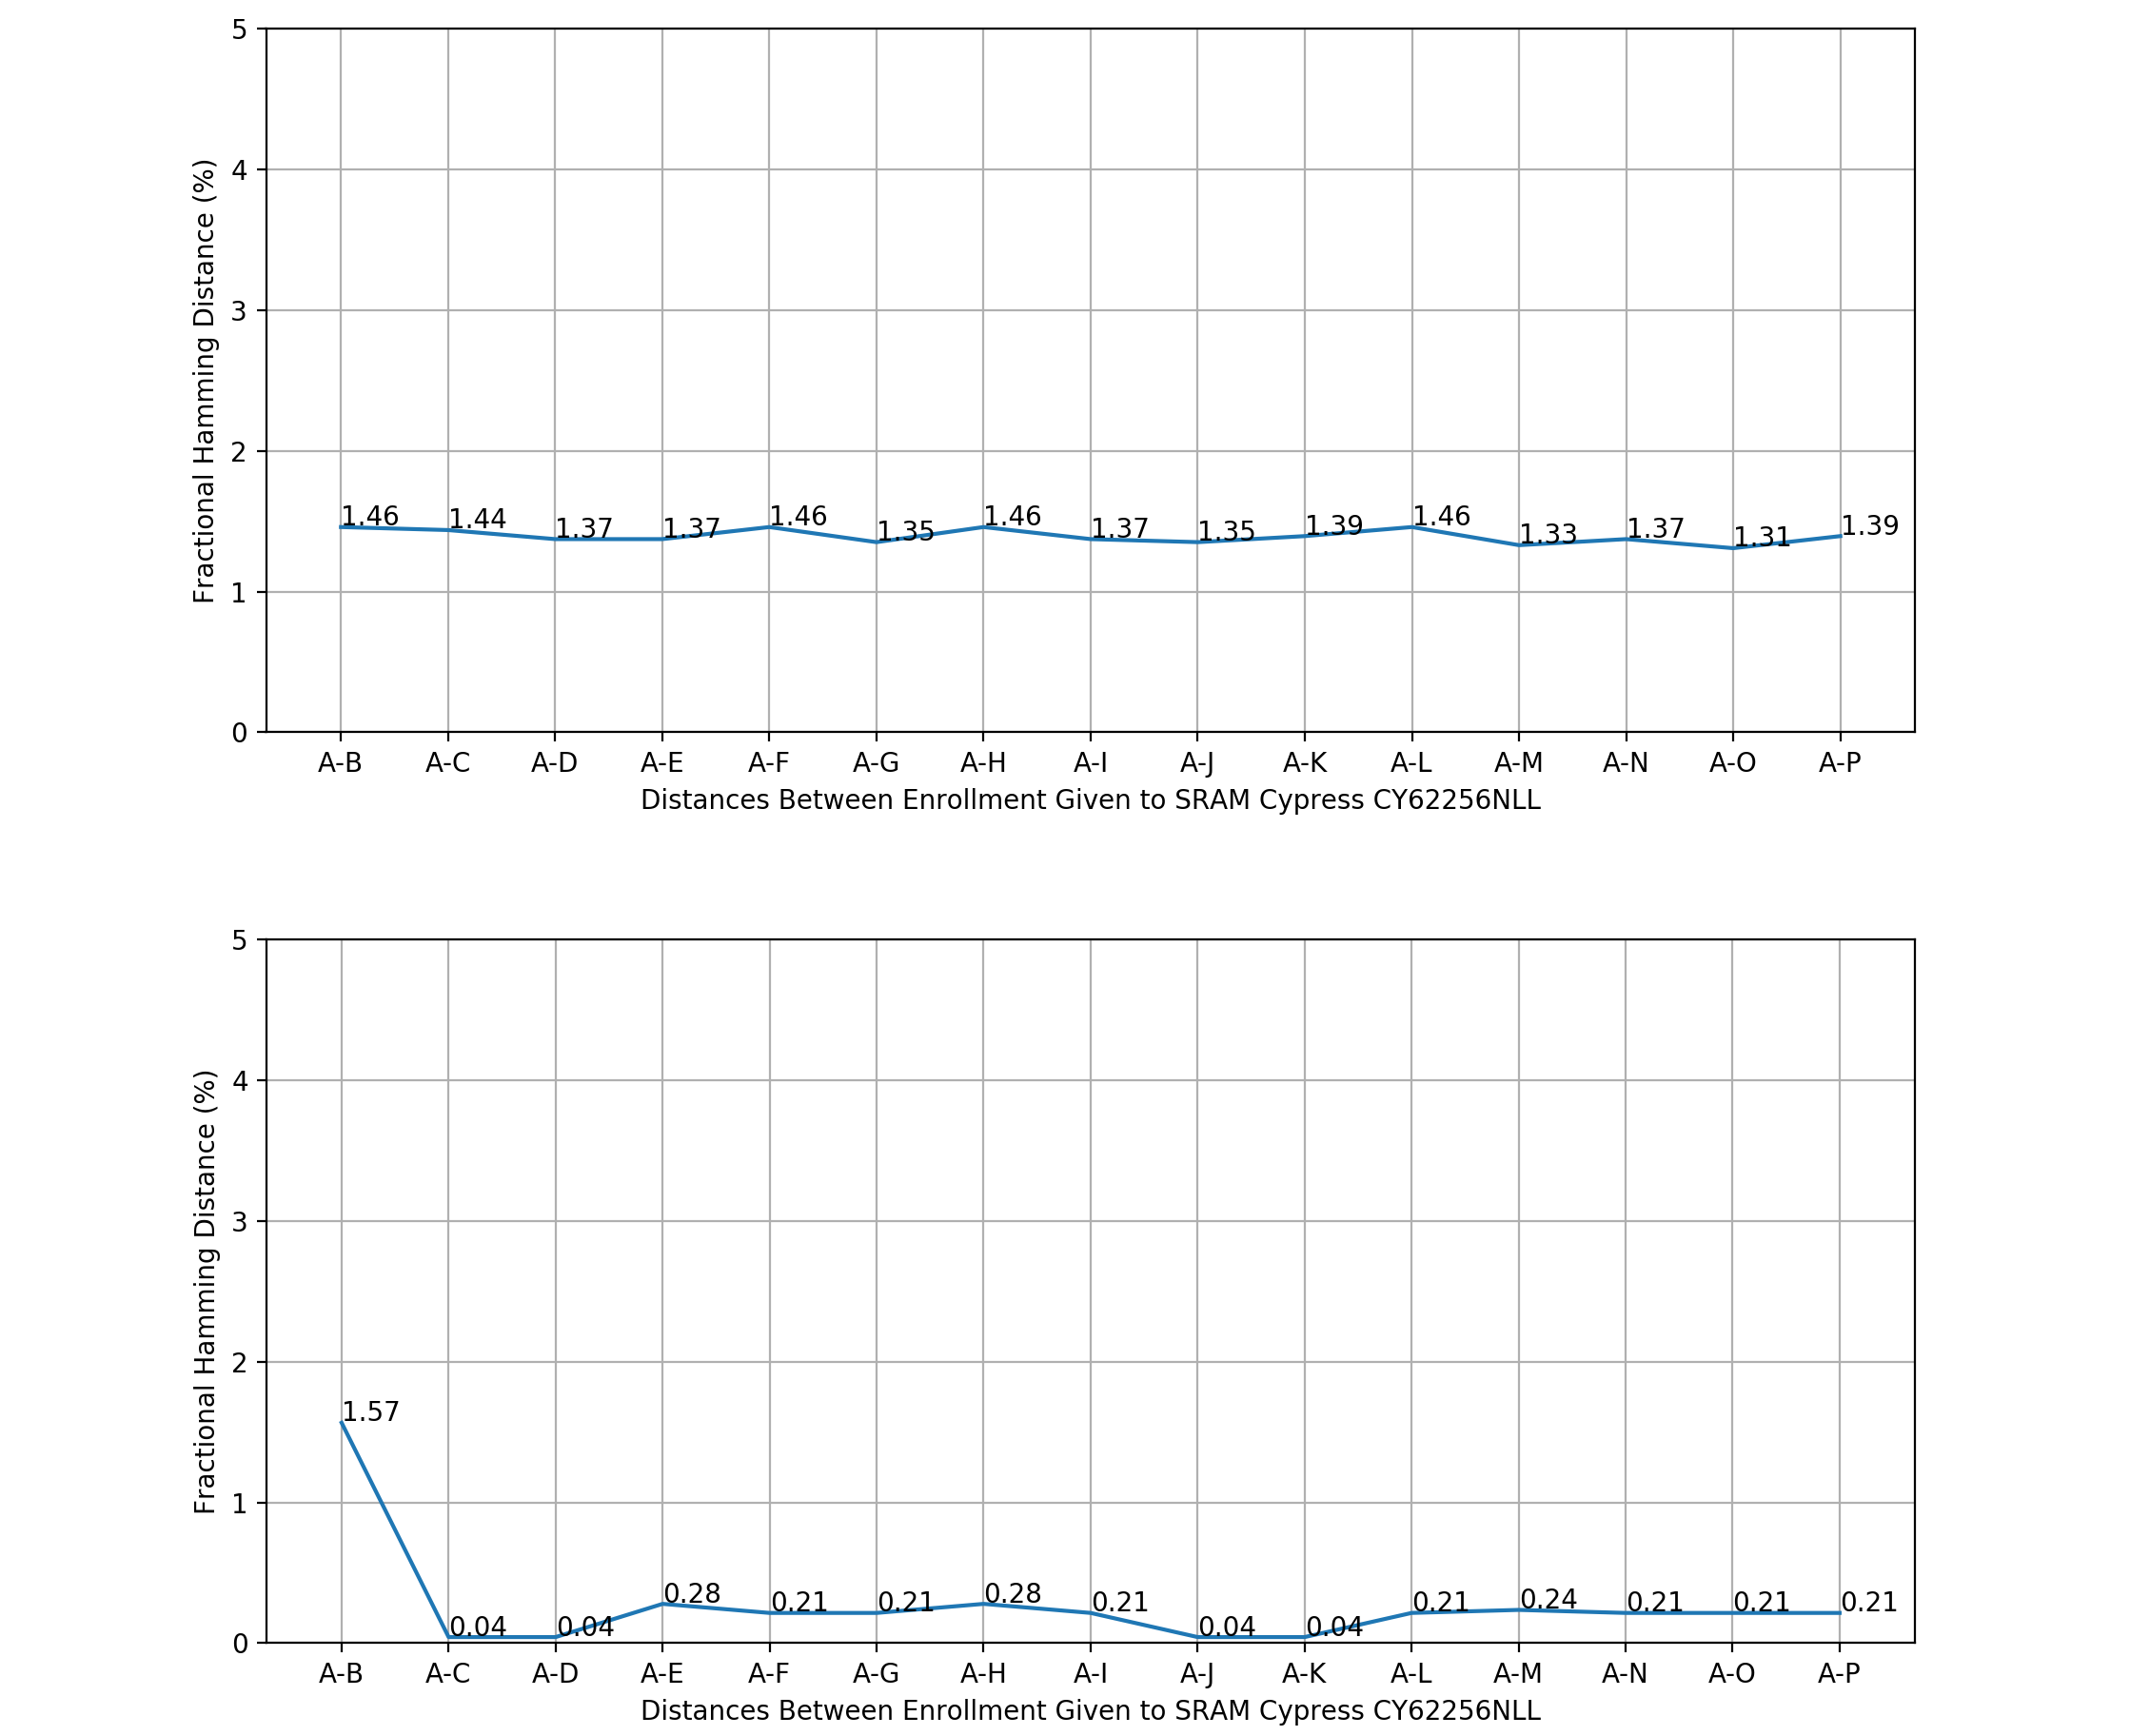
\includegraphics[width={1.1\textwidth}]{images/cy62256nll_hd_intra_time_stable}}
    \caption{Time interval testing results on SRAM Cypress CY62256NLL. The top figure is the testing result on stable bits generated using neighbor analysis, while the bottom one is tested on stable bits generated using data remanence approach. Index A on x-axis refers to enrollment on day 1, B on day 2, etc. Index A-B refers to fractional hamming distance between enrollment on day 1 and day 2.}
    \label{fig:test_stable_cy62256nll}
\end{figure}

\begin{figure}[tph!]
    \centerline{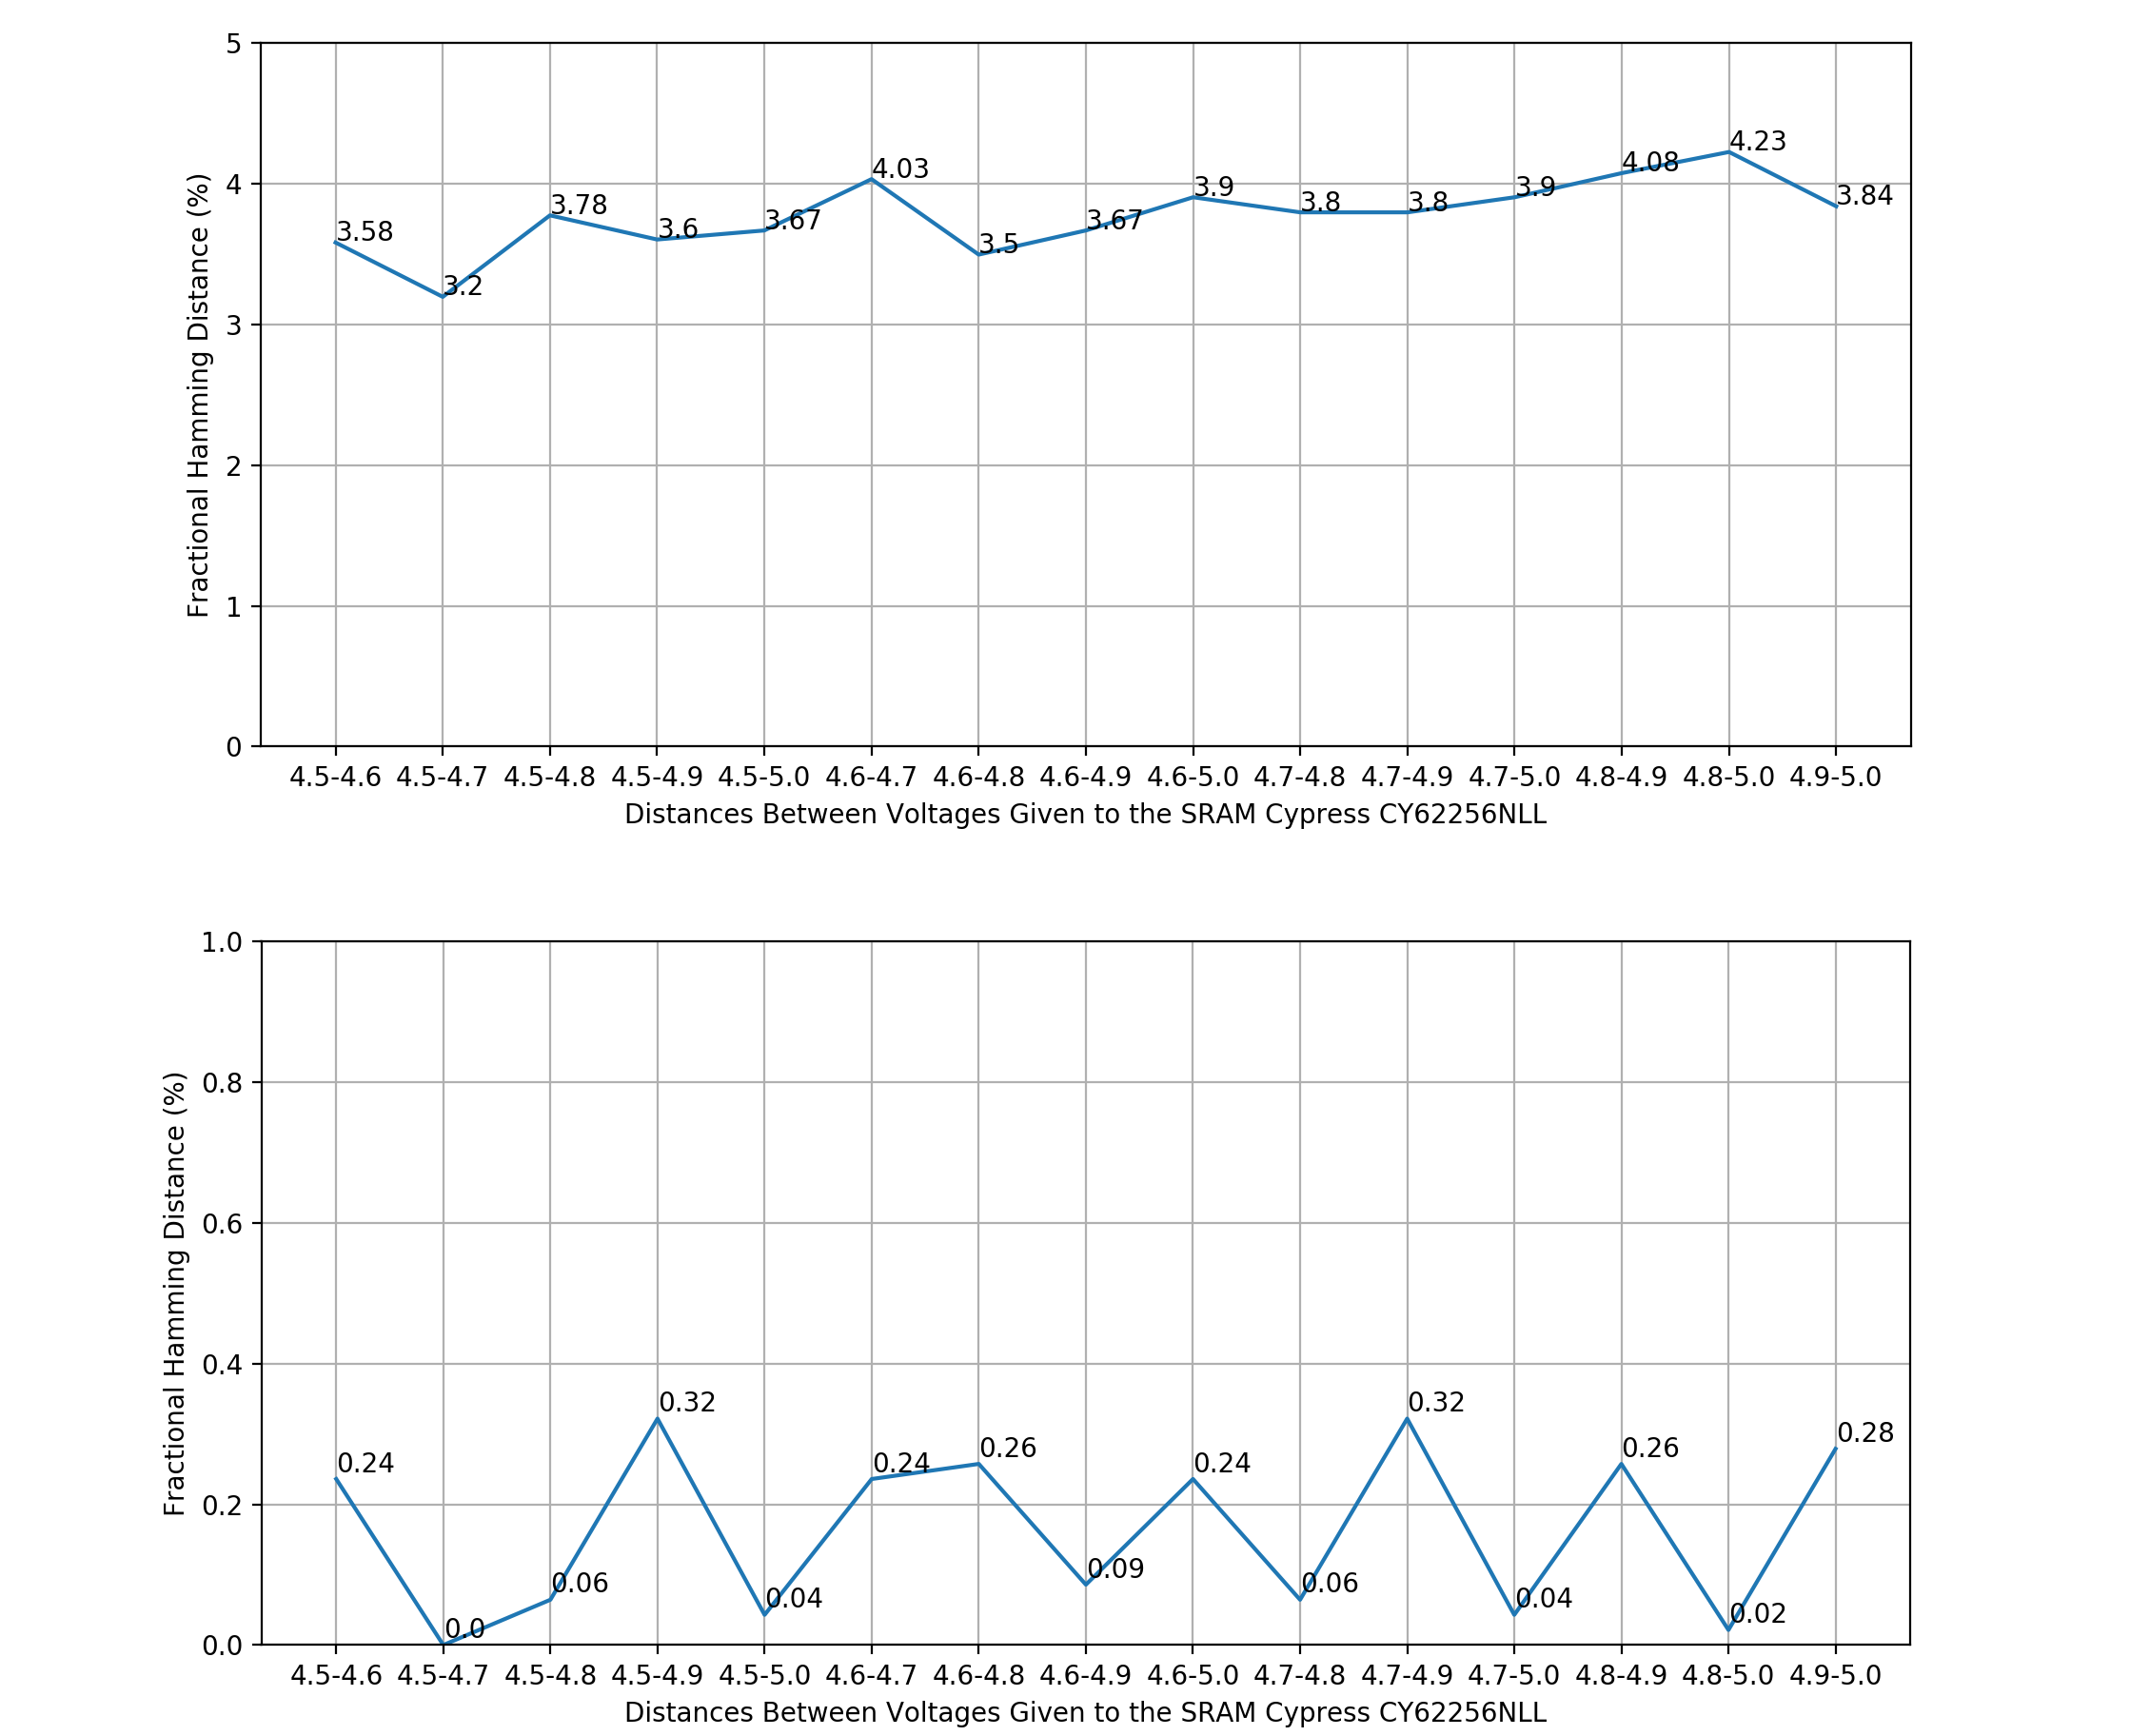
\includegraphics[width={1.1\textwidth}]{images/cy62256nll_hd_intra_voltage_stable}}
    \caption{Voltage variation testing results on SRAM Cypress CY62256NLL. The top figure is the testing result on stable bits generated using neighbor analysis, while the bottom one is tested on stable bits produced by data remanence approach. Index on x-axis refers to two different voltages, e.g. 4.5-4.6 means the fractional hamming distance between enrollment on voltage 4.5V and voltage 4.6V.}
    \label{fig:test_stable_cy62256nll_voltage}
\end{figure}

\subsubsection{Microchip 23LC1024}
\begin{itemize}
  \item Neighbor Stability Analysis\newline
  To get 4662 bits, there are three categories included; rank similar or higher than 6 with 493 bits, rank 5 with 669 bits, and rank 4 with 3500 bits.
  During testing on variated voltage and time interval, the stable bits generated using neighbor stability analysis show a poor performance by having maximum 2389 bits changing  (HD\textsubscript{intra} 51.24\%) which also produces an overlap between HD\textsubscript{intra} and HD\textsubscript{inter}. The maximum difference is produced when the difference between enrollment is 8 days.

  \item Data Remanence Approach\newline
  To get 4662 bits, strong 1's are generated using power down period of 0.185 seconds, while strong 0's are calculated when 0.27 seconds are used as the power down period. The difference between power down period during generation of strong 1's and strong 0's is because the number of 1's that flipped fast are more compared to 0's. This is also related to the 0's and 1's distribution during normal initialization (0's count for 30\% and 1's filled 70\%).
  Similar to the previous algorithm, the stability of bits produced by using this algorithm is also not good. The worst change happens when 8 days is used as the time interval between testing, showing as many as 2328 bits (HD\textsubscript{intra} 49.93\%) and also introduce an overlap between HD\textsubscript{intra} and HD\textsubscript{inter}.
\end{itemize}

\subsubsection{Cypress CY62256NLL}
\begin{itemize}
  \item Neighbor Stability Analysis\newline
  To get 4662 bits, there are six categories included; rank similar or higher than 16 with 712 bits, rank 15 with 350 bits, rank 14 with 502 bits, 726 bits of rank 13, 1104 bits of rank 12, and 1268 bits of rank 11.
  Under the voltage and time interval variation, the stable bits generated using neighbor stability analysis show decent reliability by having maximum 197 changing bits (HD\textsubscript{intra} 4.23\%) when the data is gathered on voltage 4.8V and 5V.

  \item Data Remanence Approach\newline
  Unlike SRAM 23LC1024, power down period when enrolling strong 1's and 0's on CY62256NLL is not different. To get 4662 stable bits, both are enrolled using power down period 0.34 seconds.
  During the voltage and time interval variation, the stable bits produced by using algorithm also shows a promising result. It only accounts for maximum 73 bits difference (HD\textsubscript{intra} 1.56\%).
\end{itemize}


\subsubsection{Stability Test Conclusion}

Based on these results, SRAM Cypress CY62256NLL is shown to be a reliable SRAM candidate for PUF due to its well distribution of 1's 0's inside its memory and small variance when tested on various voltage and time interval between enrollment, especially the stable bits produced by data remanence analysis which has HD\textsubscript{intra} less than 2\% on any testing. If Cypress CY62256NLL is used as the root-of-trust to produce PUF-generated key, the key is ensured to always have the same value since the key generation scheme can tolerate up to 12.7\% while the error rate of stable bits of Cypress CY62256NLL produced by data remanence algorithm is always less than 2\%.
Sadly, the other SRAM, SRAM Microchip 23LC1024, has displayed a poor performance to be eligible as a PUF candidate. Unbalanced 1's and 0's distribution and large HD\textsubscript{intra} when the stable bits are tested (larger than the maximum error capability of the key generation scheme, and even introduces an overlap between HD\textsubscript{intra} and HD\textsubscript{inter}) are two main reasons why this SRAM is not recommended to use as a PUF candidate.

These different results between two types of SRAMs lead us to a thinking that the SRAM size and the technology used in SRAM manufacturing affects a lot of SRAM quality as a PUF candidate. For example, Cypress CY62256NLL has significantly larger size than Microchip 23LC1024 (a rough approximation results in 13.38 times larger). Cypress CY62256NLL also has a smaller capacity (256 kbit) than Microchip 23LC1024 (1024 kbit). In addition, Cypress CY62256NLL is produced using an older technology (90nm) compared to Microchip 23LC1024 which has a higher chance to be produced using a newer technology since it has a much smaller size but larger memory size than Cypress CY62256NLL (there is no information on manufacturing technology used in the production on their websites and the Microchip 23LC1024 manual descriptions). From these explanations, we can conclude that Cypress CY62256NLL has less density than Microchip 23LC1024. These reasons lead us to a confirmation of density effects  explained in Section \ref{ch:sram_noise} which says the more dense an SRAM, the more environments affect the performance of the SRAM. But does it mean that SRAM PUF cannot be produced using an SRAM with a high density? This seems untrue due to some SRAM PUF references mentioned a newer technology in their PUF constructions, e.g. Cortez et. al. in \cite{7102498} use SRAMs which produced using 32nm and 45nm (sadly, there is no information on the type and manufacturer of their tested SRAMs). Moreover, as mentioned in Section \ref{ch:prev_experiments}, the experiments done in \cite{Schrijen:2012:CAS:2492708.2493033} shown that an older manufacturing technology does not always produced a more stable SRAM (Cypress CY7C15632KV18 (65nm) is more stable than Virage HP ASAP SP ULP 32-bit (90nm), even though the most stable is IDT 71V416S15PHI which produced using 180nm technology).
Furthermore, since every company always has their own way of dealing with noises introduced by high density level, we cannot conclude that high density level always lead to low quality of an SRAM as a PUF candidate. Now, this lead to another questions, what is the main criteria if an off-the-shelf SRAM is going to be used a PUF candidate? Should we trust specific company such as Cypress and mistrust another company like Microchip? Or do we need to look into specific product to determine whether an SRAM is suitable for a PUF component? Should we always prefer SRAMs with less density?
% Now, this also brings to other questions, what is the optimum density for an off-the-shelf SRAM to be valid as a PUF candidate?
We suggest the communities and the academics to study these problems further.

Another conclusion that can be retrieved is that data remanence analysis is proven to be a better bit selection algorithm than neighbor analysis which also confirms similar claim by Muqing et. al. \cite{liu_zhou_tang_parhi_kim_2017}. Futhermore, based on this outcome, further testing shown below are only done on SRAM Cypress CY62256NLL and the stable bits used are generated using the data remanence algorithm.

\section{Testing on Bits Locations as A Challenge}
In this section, the testing results on our proposed PUF challenge is presented. As mentioned in the previous chapter, bits locations is selected as the PUF challenge in our application. The test was done on SRAM Cypress CY62256NLL. Cypress CY62256NLL itself has a capacity to store 262144 bits. The number of bits required in a challenge is 2331 bits (the length of the bits required to generate 256 bits key when using scheme shown in Figure \ref{fig:key-generation-scheme}). Using Equation \ref{bits} explained in previous chapter, there are $P(262144, 2331)=\frac{262144!}{\left( 262144-2331 \right) !}\approx 10^{12626}$ possible combinations.

The selected experiment to test this challenge is by calculating the HD\textsubscript{inter} among five SRAMs. Figure \ref{fig:cy62256cy62256nll_hd_inter_stable_remanences} shows the result of this experiment. As shown in that figure, the HD\textsubscript{inter} is ranging between 35.26\% until 46.93\%, with average 42.08\%. Since there is no overlap between HD\textsubscript{intra} (shown on Section \ref{ch:hd_intra_stable}) and HD\textsubscript{inter}, this result shows that using bits locations as a challenge is sufficient to distinguish an SRAM from another.

\begin{figure}[tph!]
    \centerline{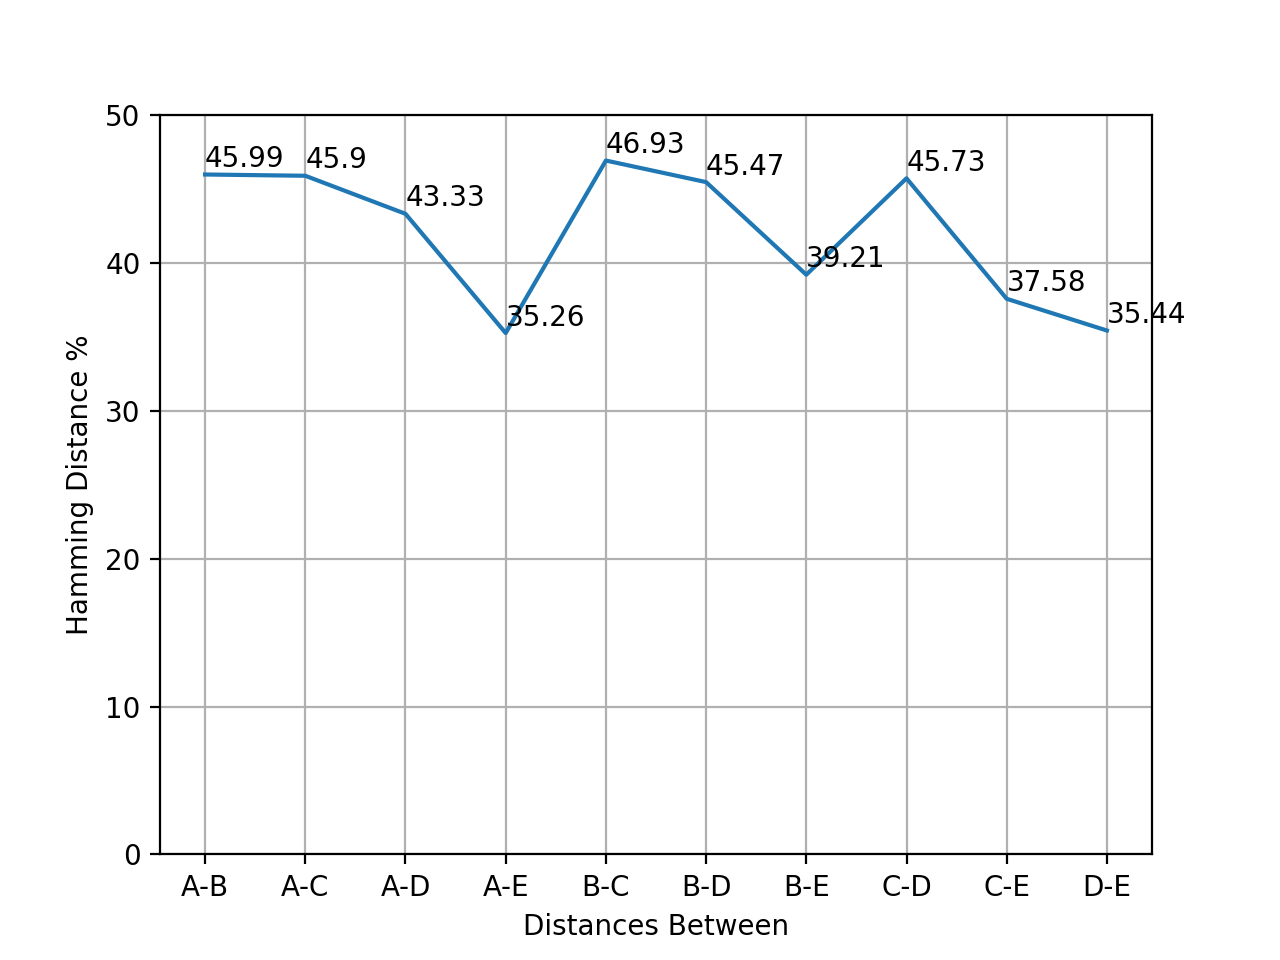
\includegraphics[width={0.9\textwidth}]{images/cy62256nll_hd_inter_stable_remanences}}
    \caption{HD\textsubscript{inter} among five SRAMs Cypress CY62256NLL. }
    \label{fig:cy62256cy62256nll_hd_inter_stable_remanences}
\end{figure}

\section{Complete Enrollment and Reconstruction Scheme}\label{ch:complete_enrollment_scheme}
Based on the experiment results shown before, we construct a complete enrollment and reconstruction scheme. The enrollment scheme has a goal to create challenge and helper data which will be used in our proposed secure data and key storage scheme (further explanation is available on Section \ref{chp:data_protection_scheme}). The reconstruction scheme has a function to reconstruct the PUF-generated key. Details on the key reconstruction can be seen on Figure \ref{fig:scheme-data-protection} and Figure \ref{fig:key-generation-scheme} in previous chapter.

Similar to the automatic profiling system, the enrollment scheme also consists of a PC, act as a master, and an Arduino connected to an external SRAM component which acts as a slave. The PC side will run Python codes while Arduino side requires Arduino codes.
Our complete enrollment scheme is shown in Figure \ref{fig:enrollment}. We also present Figure \ref{fig:cy62256nll_scheme_sd} to show how to connect an Arduino Mega 2560, an SRAM Cypress CY62256NLL and a microSD.

The enrollment scheme starts by locating stable bits using bit selection algorithm. The chosen bit selection algorithm is data remanence analysis due to its better result and shorter time needed compared to neighbor analysis. Using this algorithm, we detect the position of 4662 stable bits. Afterwards, these stable bits are shuffled to form a set of 2331 bits locations which will be used as the PUF challenge. Using Equation \ref{bits} explained in previous chapter, there are $P(4662, 2331)=\frac{4662!}{\left( 4662-2331 \right) !}\approx 8.97\times10^{8240}$ possible stable bits combinations.
The process continues with creating the helper data based on the PUF challenge. The enrollment scheme ends with storing the helper data and the PUF challenge to a microSD. Later, if one wants to reconstruct the PUF-generated key from the helper data and the challenge, he only requires an Arduino, no PC is needed (the Arduino codes used for reconstructing the PUF-generated key is different from the Arduino codes for testing and performing the enrollment scheme when it act as a slave).

\begin{figure}[tph!]
    \centerline{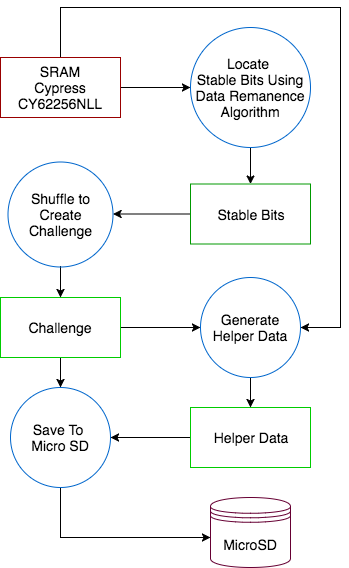
\includegraphics[width={0.5\textwidth}]{images/enrollment}}
    \caption{Complete enrollment scheme using SRAM Cypress CY62256NLL, data remanence algorithm and stable bits locations as the PUF challenge. At the end of the enrollment scheme, the challenge and helper data will be generated and saved in a microSD.}
    \label{fig:enrollment}
\end{figure}

\begin{figure}[tph!]
    \centerline{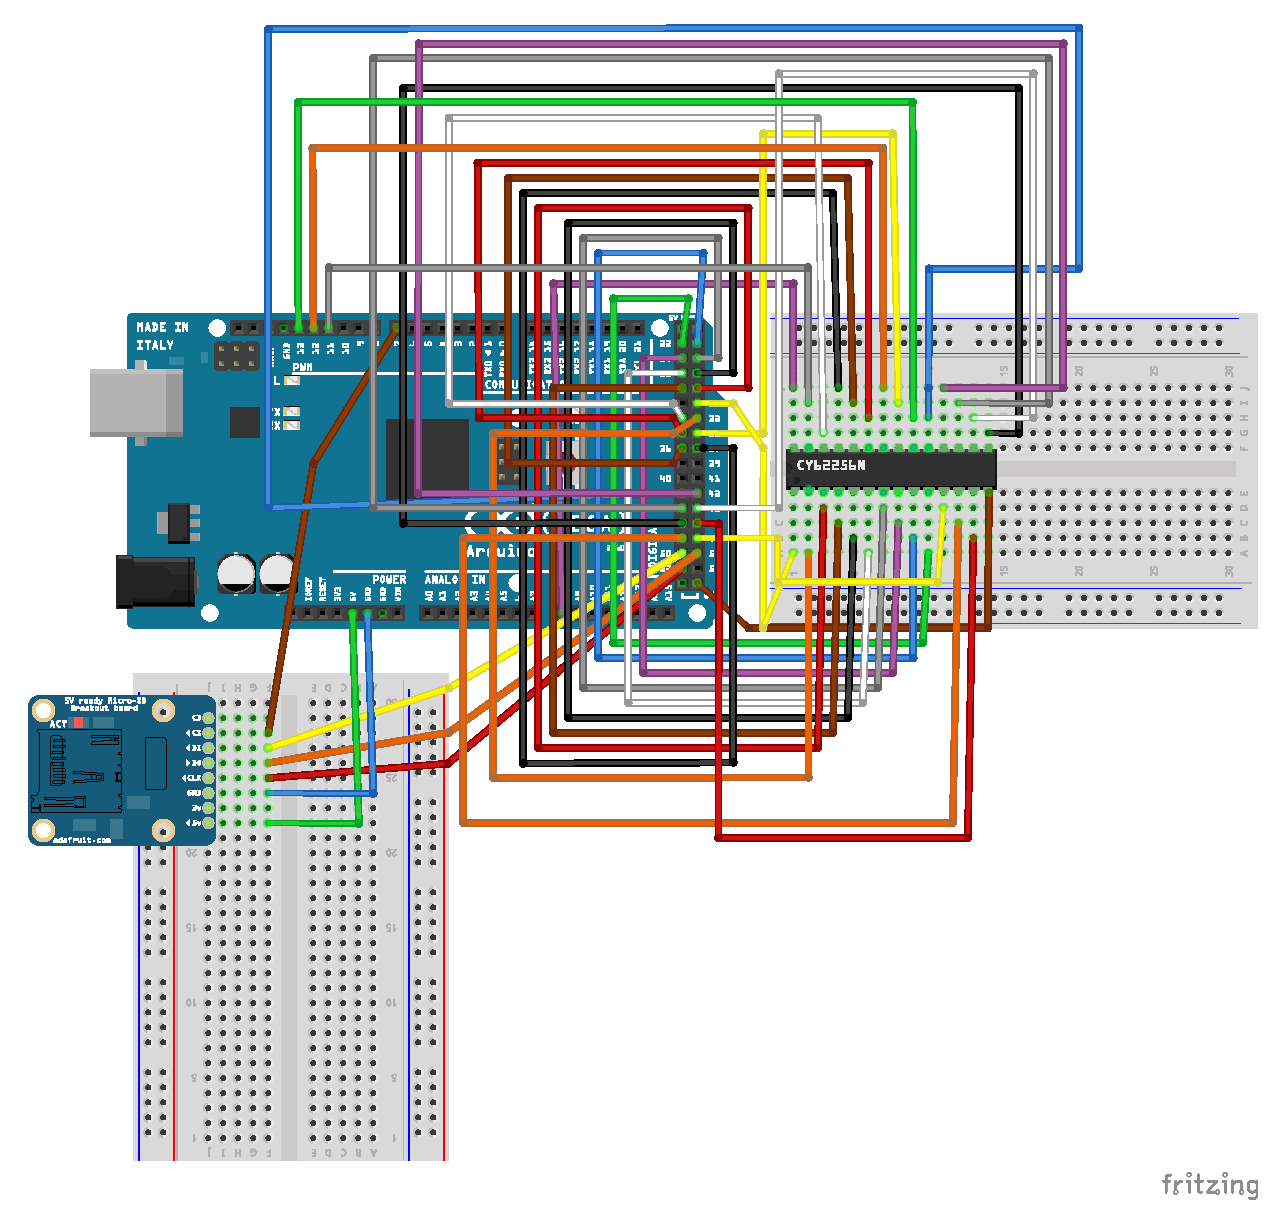
\includegraphics[width={\textwidth}]{images/CY62256-new-SD_bb}}
    \caption{An illustration on how to connect an Arduino Mega 2560 with an SRAM Cypress CY62256NLL and a microSD.}
    \label{fig:cy62256nll_scheme_sd}
\end{figure}


\section{Procedure on Developing SRAM PUF-Based Applications}\label{ch:procedure_develop}
After presenting the complete enrollment scheme, we also come up with a procedure to develop SRAM PUF-based applications using any off-the-shelf SRAM.
Similar to the complete enrollment scheme, this procedure scheme also requires a PC, acting as a master, and an Arduino connected to an external SRAM component which acts as a slave. The PC side will run Python code. To reconstruct the PUF-generated key, similar to the enrollment scheme, one also only need an Arduino, no PC is needed.
This procedure will check whether the quality of the off-the-shelf SRAM is sufficient as a PUF root-of-trust or not. In addition, the procedure also generates the helper data and the challenge of the SRAM which can be used to reconstruct PUF-generated key. Using this PUF-generated key, anyone can build their applications. For example, this PUF-generated key can be utilized as the root-of-trust in an authentication application. Below are the steps defined in this procedure:
% the off-the-shelf SRAM testing, enrollment and reconstruction mechanism
\begin{itemize}
  % First, one should be test the off-the-shelf SRAM quality to be a PUF component. If passed, the procedure continues to the next step which consists of enrollment-reconstruction mechanism which will be able to create a PUF-generated key. Last, using the PUF-generated key, one can develop any PUF-based application.
  \item Step 1: \textit{Test the off-the-shelf SRAM quality as a PUF component.}\newline
  This step can be started by getting any off-the-shelf SRAM from the market. Ensure that the Arduino and the PC are able to communicate perfectly with off-the-shelf SRAM. Afterwards, locate the stable bits using data remanence algorithm. Then, test the stable bits on various conditions. If the stable bits show an acceptable result, continue using this SRAM. Otherwise, abandon and try another off-the-shelf SRAM. In addition, also ensure there is no overlap between HD\textsubscript{inter} and HD\textsubscript{intra} to enable unique identification on the off-the-shelf SRAM.
  \item Step 2: \textit{Use enrollment-reconstruction mechanism which will be able to create a PUF-generated key.}\newline
  Using the enrollment scheme shown in Section \ref{ch:complete_enrollment_scheme}, one can generate the challenge and the helper data. Both the helper data and the challenge is unique to the tested SRAM component. Later, using the challenge and the helper data, one will be able to reconstruct the PUF-generated key.
  \item Step 3: \textit{Develop a PUF-based application using the PUF-generated key.}\newline
  The PUF-generated key can be applied as a root-of-trust in any application.
\end{itemize}

\section{Testing on Secure Data and Key Storage Scheme}\label{ch:testing_scheme}
To check the validity of the proposed data and key storage scheme, several testings are performed. First, the final key generated using HMAC SHA3 is checked. Afterwards, the result of the encryption and decryption using the final key is also tested. Last, the time required in the scheme is also measured. During the time measurement, the stage is divided into multiple stages to ease the analysis.

To check the validity of the final key, a comparison between the generated final key and an online HMAC SHA3 calculator \cite{hmac_calculator} is performed. As a reminder, the key for HMAC function is the PUF generated key and the message input for the HMAC is the user's password. Below is the testing result:
\begin{itemize}
  \item PUF generated key: \seqsplit{d20f5656bf436516cd0f3d2e734851dc537df51897484128ccae67ee1310f69b}
  \begin{itemize}
    \item user's password: 70617373776f7264\newline
    final key: \seqsplit{084536fcb3135af89e1e32d423156511f13e52246acaa591b1d4115666727814}\newline
    valid: yes
    \item user's password: 6b6f6e746f6c6b61626568\newline
    final key: \seqsplit{1d1e467224d72c81ede61fcd5d1ac10535f3ebafa6e9f0d5086e6086a30787c7}\newline
    valid: yes
    \item user's password: \seqsplit{71776572747975696f706173646667686a6b6c7a786376626e6d}\newline
    final key: \seqsplit{dda21605fc56b55659cffdf57f5453a9e380aa7bd78fe52b7dc64ff4515ff4a0}\newline
    valid: yes
  \end{itemize}
  \item PUF generated key: \seqsplit{35e2f312bd28a36a359eb1a1e37f212d17da41a5b17cb2c642f5fd8e42bbd4f0}
  \begin{itemize}
    \item user's password: 70617373776f7264\newline
    final key: \seqsplit{c2892f1b1d52d59549591d410a40527b265b91d444d2032f28ce7374f7246152}\newline
    valid: yes
    \item user's password: 6b6f6e746f6c6b61626568\newline
    final key: \seqsplit{ec85915ae65f3e5141128a520327c4d5cd3119cb6769fddd948d3061dfb6fed9}\newline
    valid: yes
    \item user's password: \seqsplit{71776572747975696f706173646667686a6b6c7a786376626e6d}\newline
    final key: \seqsplit{da9e28f76754dcd4946c1343a3dd8550338d98e46d3a11e09f903204044ac9c7}\newline
    valid: yes
  \end{itemize}
\end{itemize}

After checking the validity of the final key, a testing on encryption and decryption using the final key is performed. The input data on this testing is user’s key. To check the validity of the ciphertext, an online encryption calculator \cite{aes_calculator} is utilized. The ciphertext result of the encryption process will be used as the input for the decryption test. If the decryption result is similar with the user’s key, then both encryption and decryption process in this scheme is valid.

\begin{itemize}
  \item user's key: \seqsplit{70617373776f726470617373776f726470617373776f726470617373776f7264}
  \begin{itemize}
    \item final key: \seqsplit{084536fcb3135af89e1e32d423156511f13e52246acaa591b1d4115666727814}\newline
    ciphertext: \seqsplit{fa656b2690ea048ae807e21fefd1c4cafa656b2690ea048ae807e21fefd1c4ca}\newline
    ciphertext validity: yes\newline
    decryption result: \seqsplit{70617373776f726470617373776f726470617373776f726470617373776f7264}\newline
    decryption validity: yes

    \item final key: \seqsplit{1d1e467224d72c81ede61fcd5d1ac10535f3ebafa6e9f0d5086e6086a30787c7}\newline
    ciphertext: \seqsplit{c007e79a23c5534eb7a5bb3841304973c007e79a23c5534eb7a5bb3841304973}\newline
    ciphertext validity: yes\newline
    decryption result: \seqsplit{70617373776f726470617373776f726470617373776f726470617373776f7264}\newline
    decryption validity: yes

    \item final key: \seqsplit{dda21605fc56b55659cffdf57f5453a9e380aa7bd78fe52b7dc64ff4515ff4a0}\newline
    ciphertext: \seqsplit{7ecc0a763eb6c263c84e80307168dbd47ecc0a763eb6c263c84e80307168dbd4}\newline
    ciphertext validity: yes\newline
    decryption result: \seqsplit{70617373776f726470617373776f726470617373776f726470617373776f7264}\newline
    decryption validity: yes

    \item final key: \seqsplit{c2892f1b1d52d59549591d410a40527b265b91d444d2032f28ce7374f7246152}\newline
    ciphertext: \seqsplit{63ea246ddfff00def87c1a45ed7d09d863ea246ddfff00def87c1a45ed7d09d8}\newline
    ciphertext validity: yes\newline
    decryption result: \seqsplit{70617373776f726470617373776f726470617373776f726470617373776f7264}\newline
    decryption validity: yes

    \item final key: \seqsplit{ec85915ae65f3e5141128a520327c4d5cd3119cb6769fddd948d3061dfb6fed9}\newline
    ciphertext: \seqsplit{82e3d875ba4892f639196dfc0bd0091182e3d875ba4892f639196dfc0bd00911}\newline
    ciphertext validity: yes\newline
    decryption result: \seqsplit{70617373776f726470617373776f726470617373776f726470617373776f7264}\newline
    decryption validity: yes

    \item final key: \seqsplit{da9e28f76754dcd4946c1343a3dd8550338d98e46d3a11e09f903204044ac9c7}\newline
    ciphertext: \seqsplit{ef03a64e3bd5549a78738b64ed1c6a78ef03a64e3bd5549a78738b64ed1c6a78}\newline
    ciphertext validity: yes\newline
    decryption result: \seqsplit{70617373776f726470617373776f726470617373776f726470617373776f7264}\newline
    decryption validity: yes
  \end{itemize}

\end{itemize}

Measurement of time required in this scheme is also done. During the time measurement, the scheme is divided into eight stages. Stage one is on the initialization of the libraries required to access SRAM Cypress CY62256NLL and microSD. Stage two is when the challenge and the helper data are loaded from microSD. The third one is calculated when reconstructing the PUF key. Next stage is during the derivation of the final key (derived from user's password and PUF-generated key). Stage five and stage six refers to the processes of encryption and saving ciphertext to microSD. Stage seven and stage eight refers to the procedure of reading ciphertext from microSD and the decryption process (reconstructing the user's key). The measurement result can be seen on Table \ref{tab:time_scheme}. It can be seen that the longest time required is when loading the challenge and the helper data from the microSD (stage 2), followed by the initialization stage (stage 1). Due to this significant time required, a further optimization on accessing data from microSD is suggested in possible future works.

\begin{table}[htbp]
  \centering
  \caption{Time measurement of the secure data and key storage scheme in ms.}
    \begin{tabular}{|c|c|c|c|c|}
    \hline
    \textbf{No} & \textbf{Stage 1} & \textbf{Stage 2} & \textbf{Stage 3} & \textbf{Stage 4} \\
    \hline
    1     & 1022.66 & 2205.25 & 978.15 & 33.57 \\
    \hline
    2     & 1022.65 & 2205.24 & 974.39 & 33.57 \\
    \hline
    3     & 1022.63 & 2205.25 & 981.27 & 33.57 \\
    \hline
    Average & 1022.65 & 2205.25 & 977.94 & 33.57 \\
    \hline
    \textbf{No} & \textbf{Stage 5} & \textbf{Stage 6} & \textbf{Stage 7} & \textbf{Stage 8} \\
    \hline
    1     & 0.84  & 39.96 & 13.02 & 1.72 \\
    \hline
    2     & 0.85  & 39.88 & 13.02 & 1.71 \\
    \hline
    3     & 0.84  & 39.78 & 13.01 & 1.72 \\
    \hline
    Average & 0.84  & 39.87 & 13.02 & 1.71 \\
    \hline
    \end{tabular}%
  \label{tab:time_scheme}%
\end{table}%

To ensure the functionality of the system, we also constructed test cases for the source code. The testing is only performed on the functionality of the system which does not has a direct interaction with hardware (e.g. code to read microSD and SRAM). This decision is taken because to ensure the code is properly working, the hardware has to be in a proper condition, while checking the hardware condition is sometimes problematic and cannot be automated. The quality of the test cases is shown by code coverage which generated using GCOV and LCOV. Figure \ref{fig:code_coverage} shows the code coverage result. As seen there, there are directories where the line coverage is not 100\% covered. The reasons are some directories are just library to enable code testing (folder 'gmock' and folder 'gtest', both are libraries created by Google which required to enable the testing) and one directory is a part of LLVM compiler infrastructure (folder 'v1'). Another directory which is not fully covered is 'Crypto', this folder is a library required to do the encryption, decryption, and HMAC but provides more functional than the required for constructing the system. Thus, the test is only done on the functionality that is actually needed by the system which leads to a not full percentage of code coverage.

\begin{figure}[tph!]
    \centerline{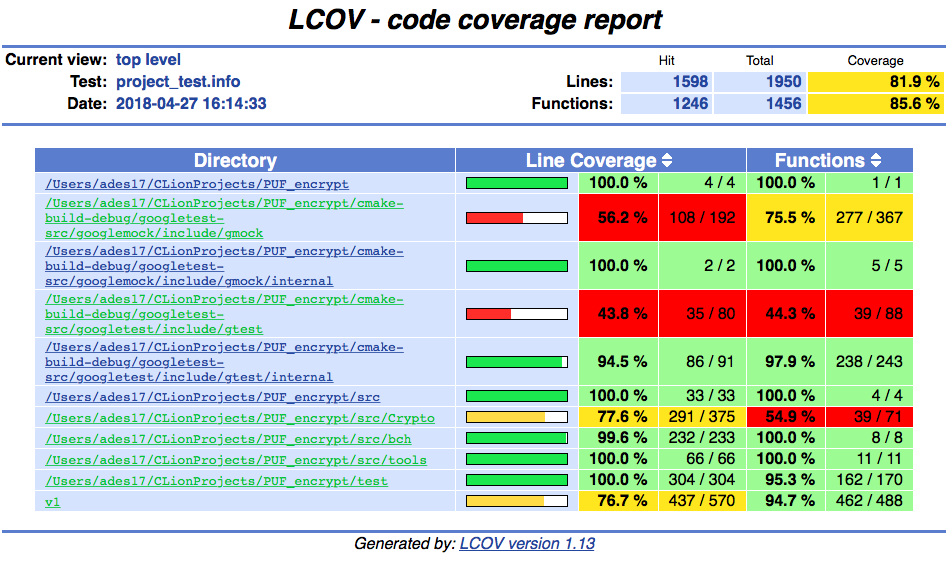
\includegraphics[width={\textwidth}]{images/code_coverage}}
    \caption{Code coverage of the constructed project.}
    \label{fig:code_coverage}
\end{figure}

% \section{Concluding Experiment with Cybercurrency}
\section{Concluding Experiment with Cybercurrency}
As the final experiment of this thesis, we present a demo of storing a private key of a cybercurrency. We believes this proves the usefulness and viability of this work for realistic use-cases. The chosen cybercurrency in this demo is Bitcoin. In Bitcoin, the private key has a length of 256-bit or 32 bytes \cite{bitcoin_key}. The experiments starts by performing an enrollment on an Arduino board with an SRAM Cypress CY62256NLL and a microSD connected to it, resulting in challenge and helper data which store in the microSD. Using the produced challenge and helper data, user creates a final key which derived from the PUF-generated key and user's password. The final key is utilized to encrypt a Bitcoin key, then the ciphertext is stored in microSD. Afterwards, the Arduino is turned off.
Later, the microSD and the SRAM are transferred to another Arduino board. The new Arduino board is powered on, then it is used to reconstruct the final key by inputing the correct user's password. Finally, the reconstructed final key is applied to the ciphertext which is loaded from the microSD. The Bitcoin key storing experiment is considered successful if the result of decryption is the same as the Bitcoin key.
Moreover, we also shows that the Bitcoin key will not be reconstructed successfully if user's password is incorrect or the SRAM is not similar with the one that use to encrypt the Bitcoin key.

This experiment was done on five SRAMs Cypress CY62256NLL which can be identified by having index 'A', 'B', 'C', 'D', and E.
The result of this experiment is shown on Appendix \ref{app:screenshot}. These figures show that the stored / secured Bitcoin key can only be reconstructed using a correct user's password and the exact SRAM that used during the storing (encryption) stage. If the SRAM is not similar with the one used for the encryption stage or the input password is inaccurate, the Bitcoin key cannot be reconstructed to the actual one.
Based on these result, we conclude that the constructed data and key storage scheme is secure and successfully built.

\section{Conclusion}
In this chapter, we provide explanations of several experiment setups and results. We start by presenting two chosen SRAMs that used in experiments; Microchip 23LC1024 and Cypress CY62256NLL. Both are tested on the effect of voltage variations regarding the HD\textsubscript{intra}, HD\textsubscript{inter}, distribution of 1's and 0's. Afterwards, the testing results on two bit selection algorithms (neighbor analysis and data remanence approach) and the reliability of the stable bits produced by these algorithms are displayed. From these experiments, we concluded that the Microchip 23LC1024 is unreliable to be a PUF candidate while Cypress CY62256NLL has a solid ground to be the root-of-trust of PUF. We also able to determine that data remanence approach can produce more stable bits compared to neighbor analysis.
The chapter continues with examination on our proposed PUF challenge. Since Cypress CY62256NLL has a capacity of 262144 bits and the required bits for PUF generation is 2331 bits, there are $P(262144, 2331)=\frac{262144!}{\left( 262144-2331 \right) !}\approx 10^{12626}$ possible challenges. We also display our complete enrollment scheme and the procedure on developing SRAM PUF-based applications using any off-the-shelf SRAM.
Moreover, we also propose a procedure to develop SRAM PUF-based applications using any off-the-shelf SRAM. The procedure consists of three main steps; test the off-the-shelf SRAM quality to be a PUF component, create a PUF-generated key using enrollment-reconstruction mechanism, and develop any PUF-based application utilizing the PUF-generated key.
Next, testing on the designed secure data and key storage scheme is shown. Last, experiment outcomes on storing Bitcoin private key conclude this chapter.


% CONCLUSIONS AND FUTURE WORK
\chapter{\chapterSix}
\label{chp:6}

\section{Conclusions}
This thesis starts by showing the potential of using SRAM PUF as a secure way to protect our key and data. Embraced with a bright prospect, it is unfortunate that the development of PUF in the real world seems to lack of public involvement. The currently available solution is usually locked to specific entities, such as companies or universities. There is no open source project available for tech enthusiast to embrace this amazing technology. Here, we initiate an open source project to develop software-based SRAM PUF technology using off-the-shelf SRAM.
% We also present an automated enrollment system. The system, inspired by the concept of master-slave, consists of an Arduino source code (act as a slave) and a python source code, perform as a master, run in PC.  Using this system, two types of SRAM are tested; Microchip 23LC1024 and Cypress CY62256NLL. Both are tested on the distribution of 0's and 1's in their cells, intra hamming distance, inter hamming distance and the effect of voltage and time interval between enrollment.

We also present testing results on two off-the-shelf SRAMs as SRAM PUF candidates; Microchip 23LC1024 and Cypress CY62256NLL. Both are tested on the distribution of 0's and 1's in their cells, intra hamming distance, inter hamming distance, and the effect of voltage variation and time interval between enrollment. Testing on two bit-selection algorithms (data remanence analysis and neighbor analysis) are also performed on both SRAMs. The testing results show that Cypress CY62256NLL is a qualified PUF candidate due to well distributed of 1's and 0's inside its memory and the stability of its stable bits produced by data remanence analysis against voltage variation and time variation between interval. Sadly, SRAM Microchip 23LC1024 has displayed a poor performance to be eligible as a PUF candidate due to unbalanced 1's and 0's distribution and large HD\textsubscript{intra} when the stable bits are tested. We believe a factor that make Cypress CY62256NLL performs better than Microchip 23LC1024 is its less density level. Unfortunetely, we cannot a hundred percent sure that high density level always make an off-the-shelf SRAM performs poorly as a PUF candidate due to some SRAM PUF references mentioned a newer technology in their PUF constructions, e.g. Cortez et. al. in \cite{7102498} use SRAMs which produced using 32nm and 45nm. Another reason is because every company always has their own way of dealing with noises introduced by high density level, thus opening a possibility that maybe SRAM produced from specific company is better than the other. We suggest the communities and academicians to study this problem further.
These experiments also confirms the claim by Muqing et. al. in \cite{liu_zhou_tang_parhi_kim_2017} which says data remanence analysis is a better bit selection algorithm than neighbor analysis.
Afterwards, based on the testing results, we introduce a PUF enrollment scheme using data remanence analysis as the bit selection algorithm which will locate the location of the stable bits and SRAM Cypress CY62256NLL as the off-the-shelf SRAM component.


% We provide an enrollment mechanism to look for stable bits which will be used as the basis for PUF application. There are two algorithms for looking stable bits tested here; neighbors analysis and data remanence approach. Based on the experiment results, in our final enrollment scheme, we present a concrete SRAM PUF enrollment using an Arduino, an SRAM Cypress CY62256NLL and a microSD with data remanence approach as the bit selection algorithm. A microSD is required to store the helper data and the PUF challenge.

In addition, an idea to create a strong PUF using SRAM is also proposed here. Using a collection of bits as a challenge, the stable bits are permutated among themselves to create a challenge which has a tremendous number of possibilities.
Due to the large CRPs, we believe this concept can be an approach to be a strong PUF even though only using SRAM PUF.

Furthermore, we also introduce a secure data protection and key storage scheme using SRAM PUF. The proposed scheme is influenced by multi-factor authentication. Using a combination of a PUF-generated key and user's password, a derived key is produced and utilized as the final key to protect user's data or/and user's key. Unlike the automated enrollment system, this scheme only consists of an Arduino source code. Evaluation on this scheme time and code size are also presented.

\section{Future Work}

There are two major parts on possible future work, first is suggestion on possible experiments to do on off-the-shelf SRAMs and second, possible improvements on our secure data protection and key storage scheme. Explanations on these two will be provided below.

\subsubsection{Possible Experiments on Off-the-shelf SRAMs}
In this thesis, the SRAM testing is only done on the effect of time interval between enrollment and voltage variation. We believe another testing on temperature and aging is required to ensure whether SRAM Cypress CY62256NLL is indeed a capable candidate for SRAM PUF. The capability to test on temperature and the aging effect is suggested to be included as an addition of our automated enrollment system.
In addition, we also encouraged others to test other types of SRAMs to enrich the knowledge of possible off-the-shelf SRAM as a PUF candidate and to check if a high density level always lead to a poor performance for an SRAM to be a PUF candidate. Doing testing on other types of SRAMs can also confirm whether a product from specific is qualified as a PUF root-of-trust or not.


\subsubsection{Improvement on Secure Data Protection and Key Storage Scheme}
As mentioned in Section \ref{ch:testing_scheme}, during the time measurement of our proposed key storage scheme, two procedures which spend significant time is the reading challenge from microSD and the initialization stages. We suggest to further optimize these stages to give a better and faster performance.

This thesis only presents an idea to secure user's data using symmetric encryption. To see similar application but using asymmetric encryption concept, one should look further to the thesis done by Akhundov \cite{haji}. He presents a public key infrastructure (PKI) concept using the PUF-generated key as the root of trust. A possible integration between our work and his work is combining our 'final' key into his construction as a root of trust.

Moreover, our secure data protection and key storage scheme is only designed to work offline. We believe by making it works in an online scenario will lead to more usable applications in real life. The first step we suggest on evolving it to be an online scheme is by providing the Arduino with an internet connection and by storing the helper data and the challenge in the cloud infrastructure. This step will reduce the necessity for the Arduino to always connected to a microSD. To reconstruct the PUF-generated key, Arduino will just have to get the challenge and the helper data from the cloud. We also advise to do extensive security analysis if it is decided to work online since the risks in an online environment are numerous.

In addition, our idea of using user's password and the PUF-generated key is not the highest level of security in multi-factor authentication. As mentioned in Section \ref{chp:2.mfa}, the most secure multi-factor authentication can be achieved when all three factors are combined together; knowledge, possession, and inherence. Since there are only two factors utilize (knowledge and possession) in this thesis' proposed secure data protection and key storage scheme, an addition of inherence factor when generating the final key can increase the security level. As mentioned in Section \ref{ris_puf}, biometric-based authentication and PUF are utilized to secure self-sovereign identity in Pouwelse and de Vos's proposed technology stack during trust creation in blockchain era. A further read on their article mentioned that there is a working prototype of fingerprint authentication using a smartphone camera. Since that project and our work share the same principle, open source and open ecosystem, we suggest integrating this fingerprint authentication into our proposed scheme to enable an even higher level of security.


% BIBLIOGRAPHY
% \addcontentsline{toc}{chapter}{Bibliography}
% \bibliographystyle{bib/latex8}
\bibliographystyle{unsrt}
% \bibliography{bib/all}
\bibliography{bib/article,bib/book,bib/inbook,bib/inproceedings,bib/misc,bib/mscthesis}


\appendix

\chapter{Screenshot of Secure Data and Key Storage Scheme}
\label{app:screenshot}
Appendix body

% SRAM A
\begin{figure}[tph!]
    \centerline{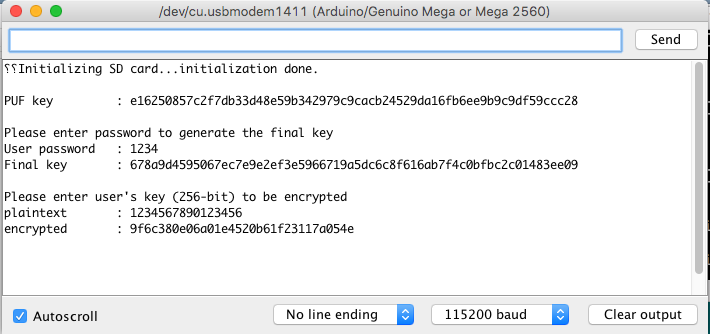
\includegraphics[width={\textwidth}]{images/A_encrypt}}
    \caption{Screenshot of the Bitcoin key storing experiment during encryption stage using SRAM Cypress CY62256NLL 'A'.
    User's password is 'password' and the Bitcoin key (user's key) is 'passwordpasswordpasswordpassword'.}
    \label{fig:A_encrypt}
\end{figure}

\begin{figure}[tph!]
    \centerline{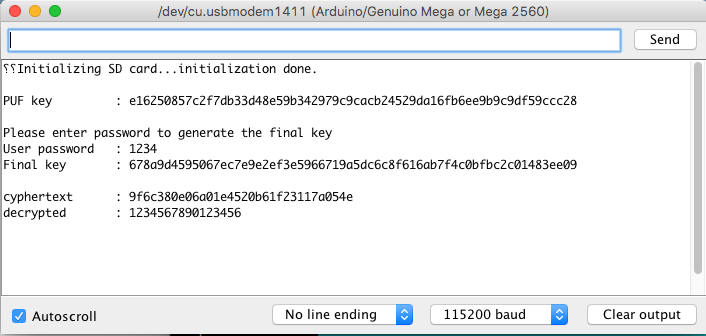
\includegraphics[width={\textwidth}]{images/A_decrypt_correct}}
    \caption{Screenshot of the Bitcoin key storing experiment during decryption stage. The Bitcoin key 'passwordpasswordpasswordpassword' is previously secured by using SRAM Cypress CY62256NLL 'A' and user's password 'password'.
    The Bitcoin key can be reconstructed because user's password is correct and the utilized SRAM is SRAM Cypress CY62256NLL 'A'.}
    \label{fig:A_decrypt_correct}
\end{figure}

\begin{figure}[tph!]
    \centerline{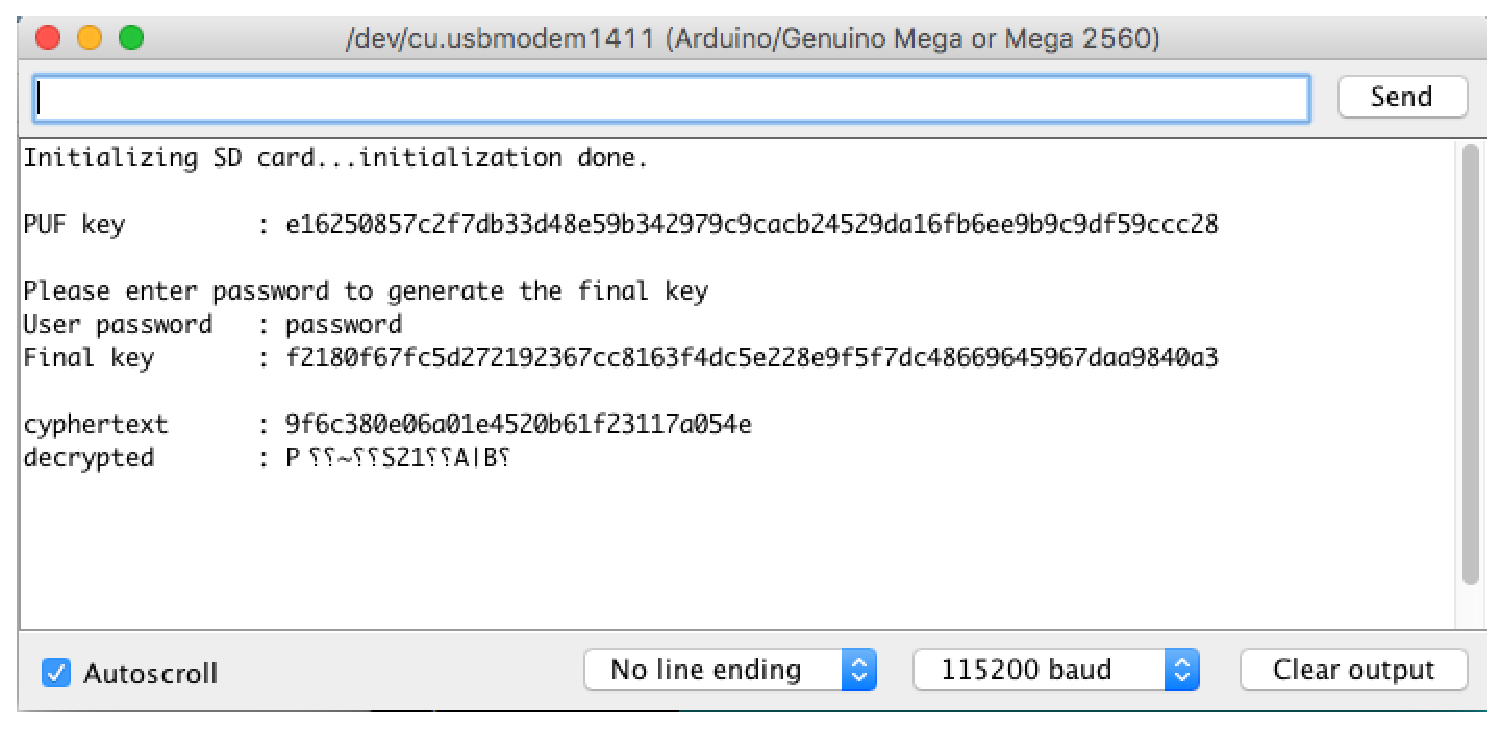
\includegraphics[width={\textwidth}]{images/A_decrypt_wrong_password}}
    \caption{Screenshot of the Bitcoin key storing experiment during decryption stage. The Bitcoin key 'passwordpasswordpasswordpassword' is previously secured by using SRAM Cypress CY62256NLL 'A' and user's password 'password'.
    Even though the utilized SRAM is the correct SRAM (SRAM Cypress CY62256NLL 'A'), the Bitcoin key cannot be reconstructed because user's password is wrong.}
    \label{fig:A_decrypt_wrong_password}
\end{figure}

\begin{figure}[tph!]
    \centerline{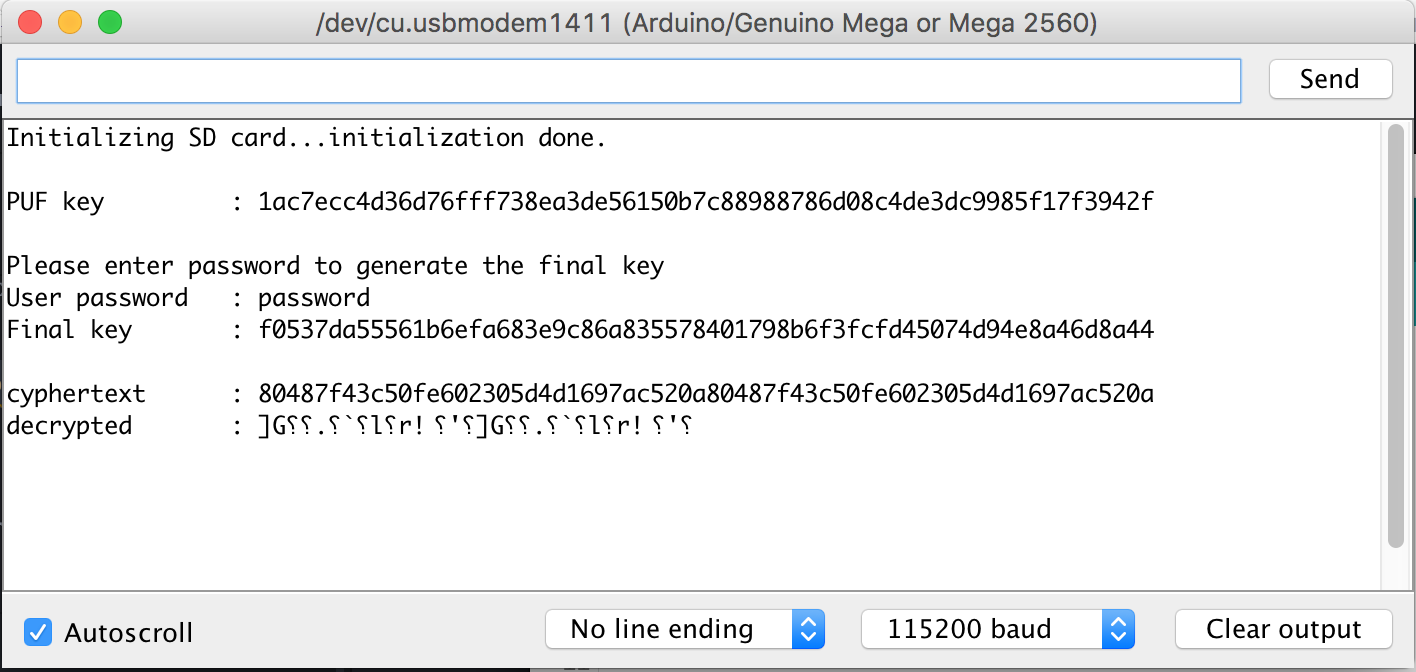
\includegraphics[width={\textwidth}]{images/A_decrypt_wrong_SRAM}}
    \caption{Screenshot of the Bitcoin key storing experiment during decryption stage. The Bitcoin key '1234567890123456' is previously secured by using SRAM Cypress CY62256NLL 'A' and user's password 'password'.
    Even though user's password is correct, the Bitcoin key cannot be reconstructed because the SRAM utilized for the decryption is SRAM Cypress CY62256NLL 'D'.}
    \label{fig:A_decrypt_wrong_SRAM}
\end{figure}

% SRAM B
\begin{figure}[tph!]
    \centerline{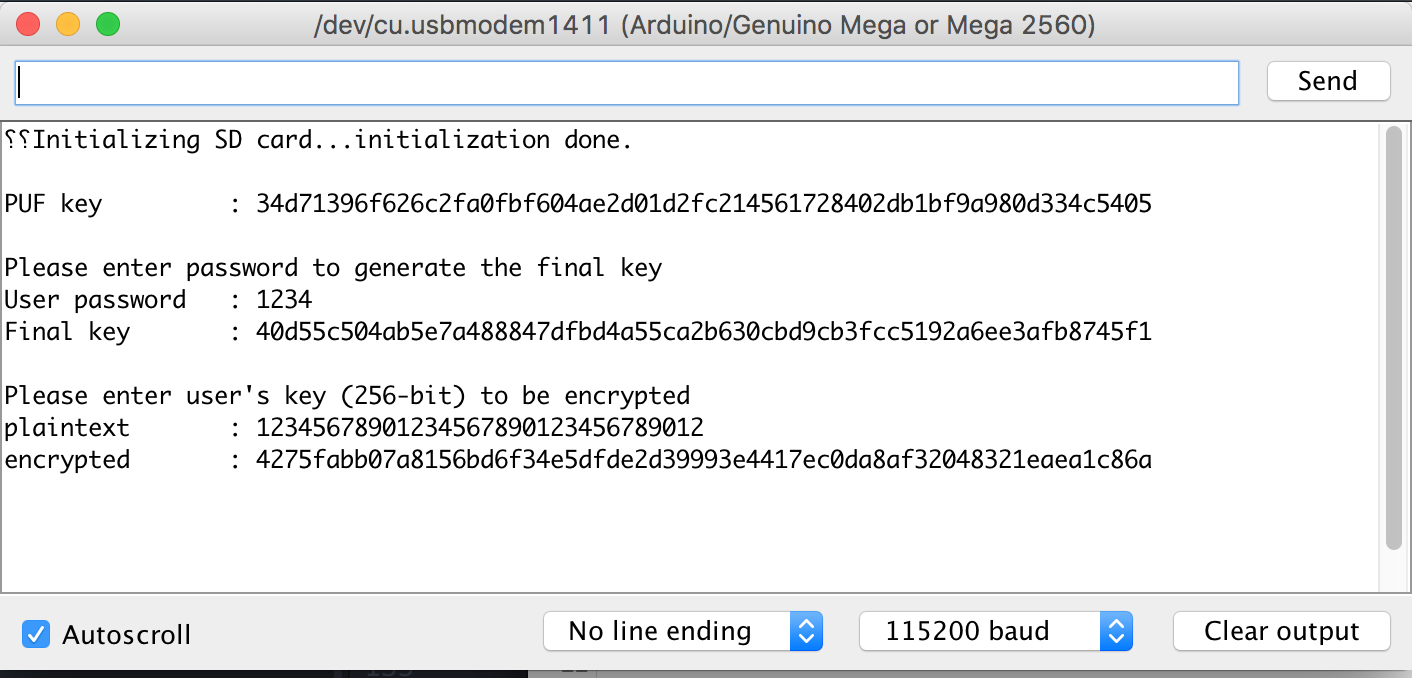
\includegraphics[width={\textwidth}]{images/B_encrypt}}
    \caption{Screenshot of the Bitcoin key storing experiment during encryption stage using SRAM Cypress CY62256NLL 'B'.
    User's password is '1234' and the Bitcoin key (user's key) is '12345678901234567890123456789012'.}
    \label{fig:B_encrypt}
\end{figure}

\begin{figure}[tph!]
    \centerline{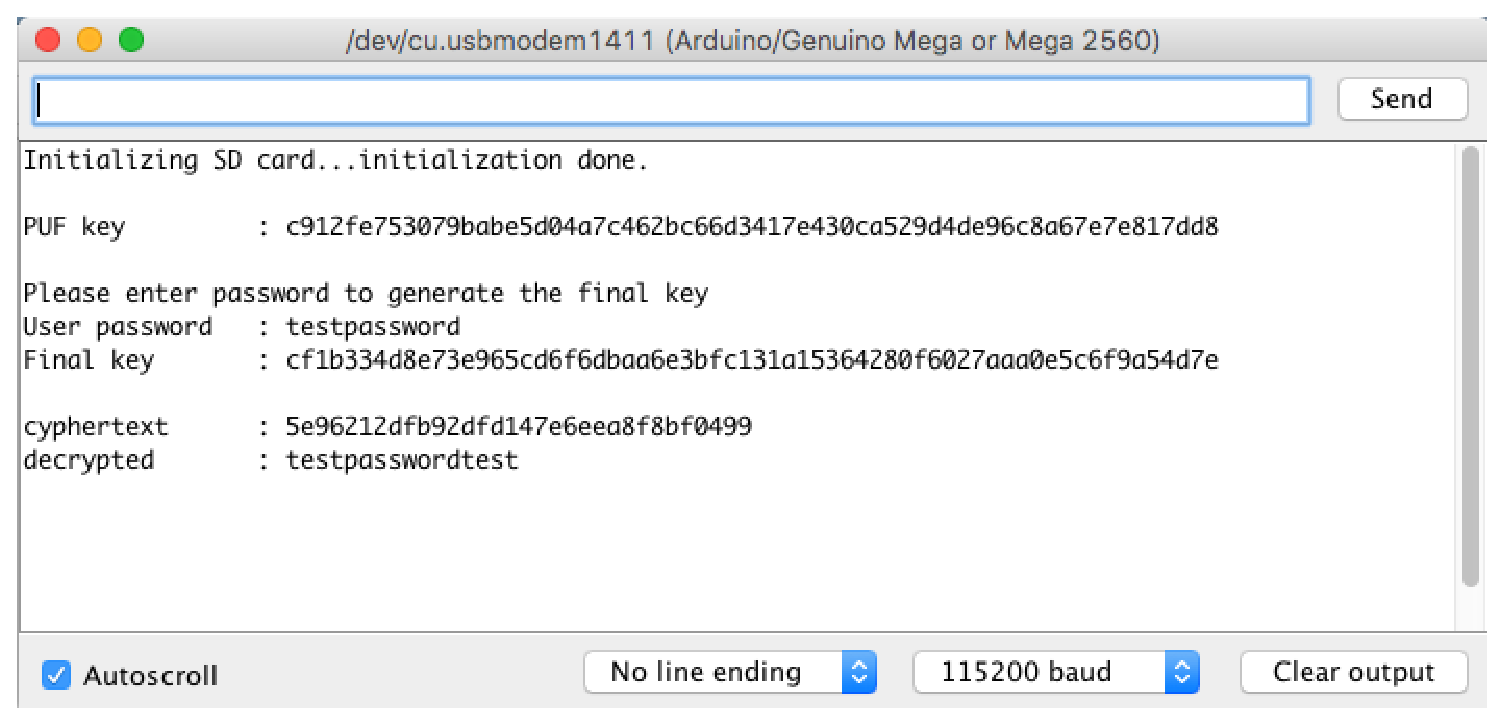
\includegraphics[width={\textwidth}]{images/B_decrypt_correct}}
    \caption{Screenshot of the Bitcoin key storing experiment during decryption stage. The Bitcoin key '12345678901234567890123456789012' is previously secured by using SRAM Cypress CY62256NLL 'B' and user's password '1234'.
    The Bitcoin key can be reconstructed because user's password is correct and the utilized SRAM is SRAM Cypress CY62256NLL 'B'.}
    \label{fig:B_decrypt_correct}
\end{figure}

\begin{figure}[tph!]
    \centerline{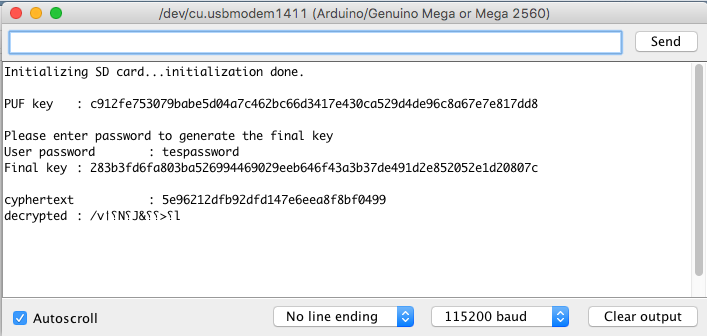
\includegraphics[width={\textwidth}]{images/B_decrypt_wrong_password}}
    \caption{Screenshot of the Bitcoin key storing experiment during decryption stage. The Bitcoin key '12345678901234567890123456789012' is previously secured by using SRAM Cypress CY62256NLL 'B' and user's password '1234'.
    Even though the utilized SRAM is the correct SRAM (SRAM Cypress CY62256NLL 'B'), the Bitcoin key cannot be reconstructed because user's password is wrong.}
    \label{fig:B_decrypt_wrong_password}
\end{figure}

\begin{figure}[tph!]
    \centerline{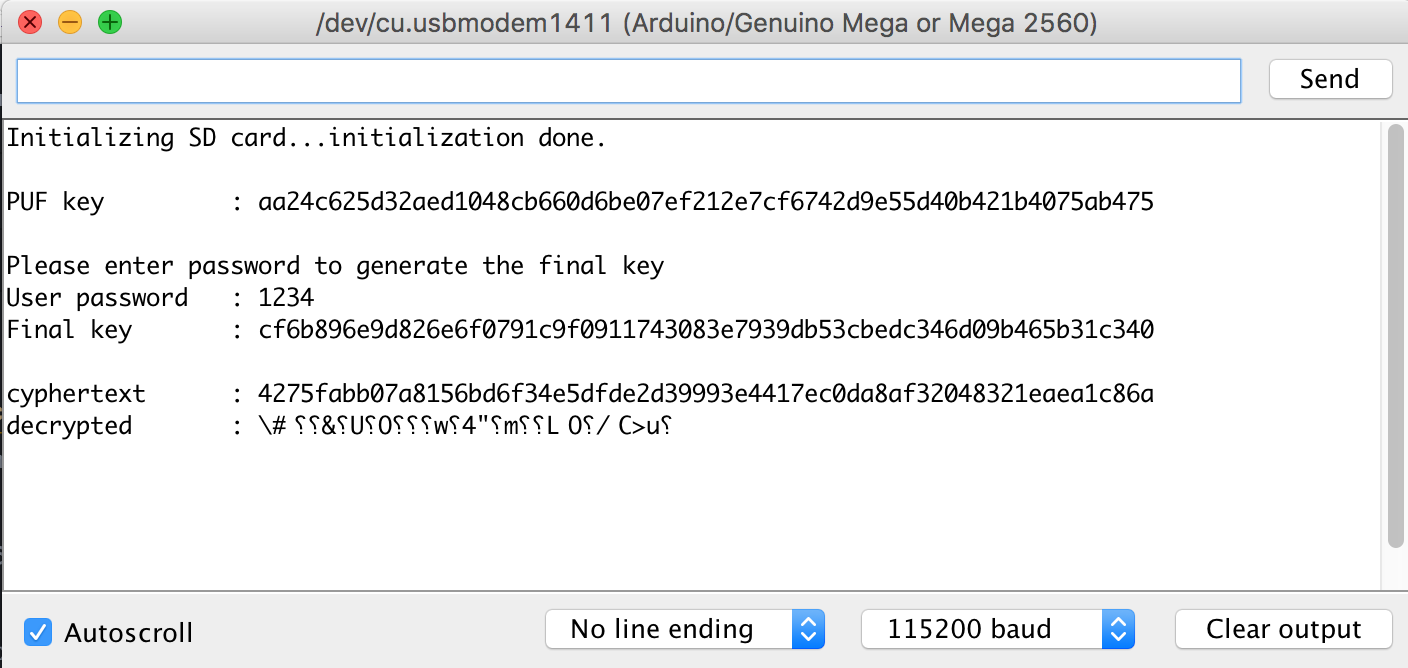
\includegraphics[width={\textwidth}]{images/B_decrypt_wrong_SRAM}}
    \caption{Screenshot of the Bitcoin key storing experiment during decryption stage. The Bitcoin key '12345678901234567890123456789012' is previously secured by using SRAM Cypress CY62256NLL 'B' and user's password '1234'.
    Even though user's password is correct, the Bitcoin key cannot be reconstructed because the SRAM utilized for the decryption is SRAM Cypress CY62256NLL 'A'.}
    \label{fig:B_decrypt_wrong_SRAM}
\end{figure}

% SRAM C
\begin{figure}[tph!]
    \centerline{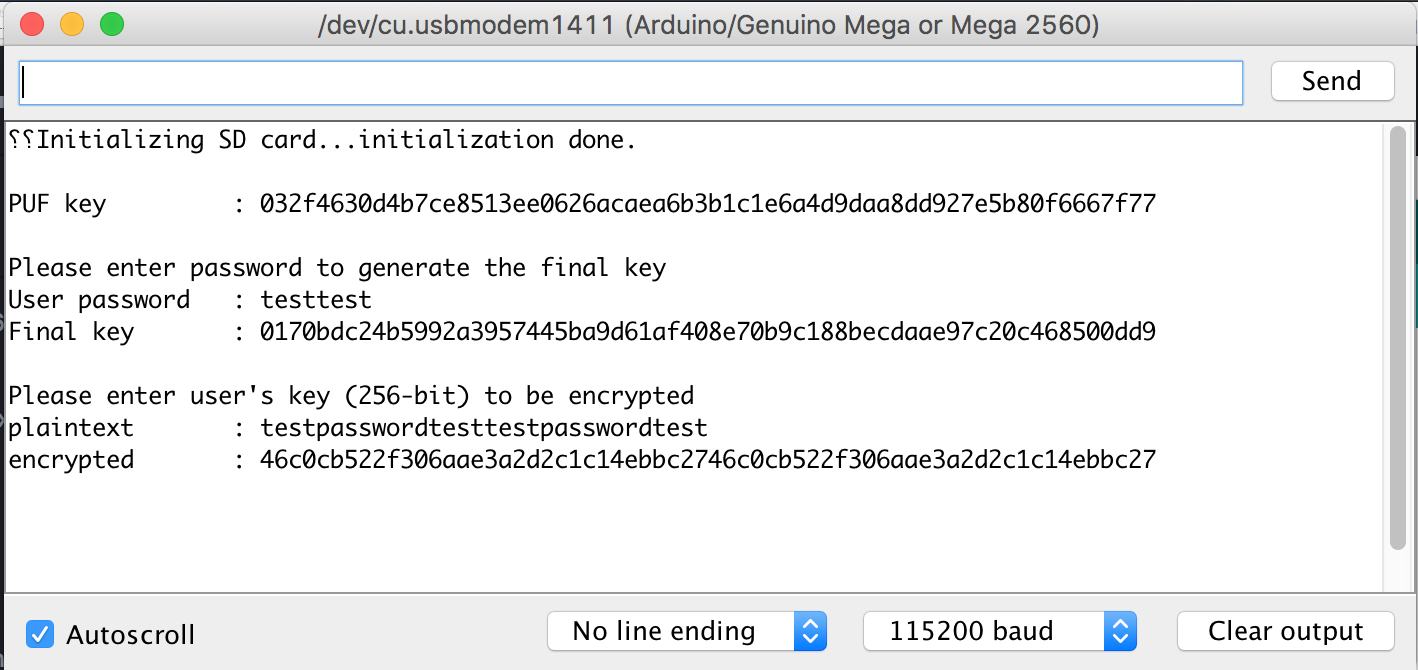
\includegraphics[width={\textwidth}]{images/C_encrypt}}
    \caption{Screenshot of the Bitcoin key storing experiment during encryption stage using SRAM Cypress CY62256NLL 'C'.
    User's password is 'testtest' and the Bitcoin key (user's key) is 'testpasswordtesttestpasswordtest'.}
    \label{fig:C_encrypt}
\end{figure}

\begin{figure}[tph!]
    \centerline{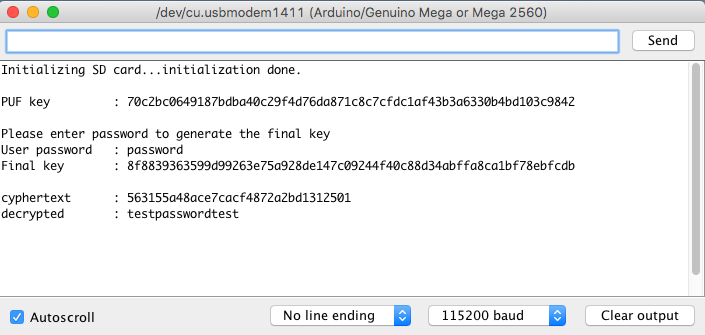
\includegraphics[width={\textwidth}]{images/C_decrypt_correct}}
    \caption{Screenshot of the Bitcoin key storing experiment during decryption stage. The Bitcoin key 'testpasswordtesttestpasswordtest' is previously secured by using SRAM Cypress CY62256NLL 'C' and user's password 'testtest'.
    The Bitcoin key can be reconstructed because user's password is correct and the utilized SRAM is SRAM Cypress CY62256NLL 'C'.}
    \label{fig:C_decrypt_correct}
\end{figure}

\begin{figure}[tph!]
    \centerline{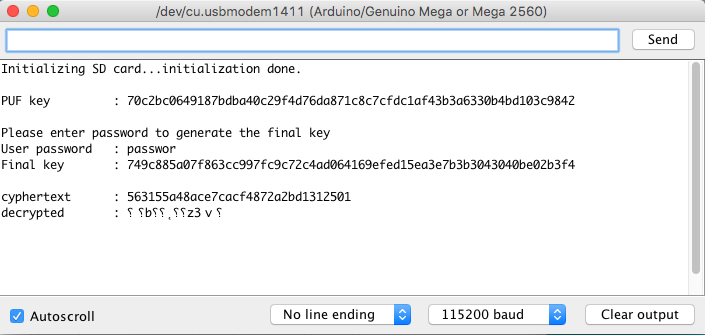
\includegraphics[width={\textwidth}]{images/C_decrypt_wrong_password}}
    \caption{Screenshot of the Bitcoin key storing experiment during decryption stage. The Bitcoin key 'testpasswordtesttestpasswordtest' is previously secured by using SRAM Cypress CY62256NLL 'C' and user's password 'testtest'.
    Even though the utilized SRAM is the correct SRAM (SRAM Cypress CY62256NLL 'C'), the Bitcoin key cannot be reconstructed because user's password is wrong.}
    \label{fig:C_decrypt_wrong_password}
\end{figure}

\begin{figure}[tph!]
    \centerline{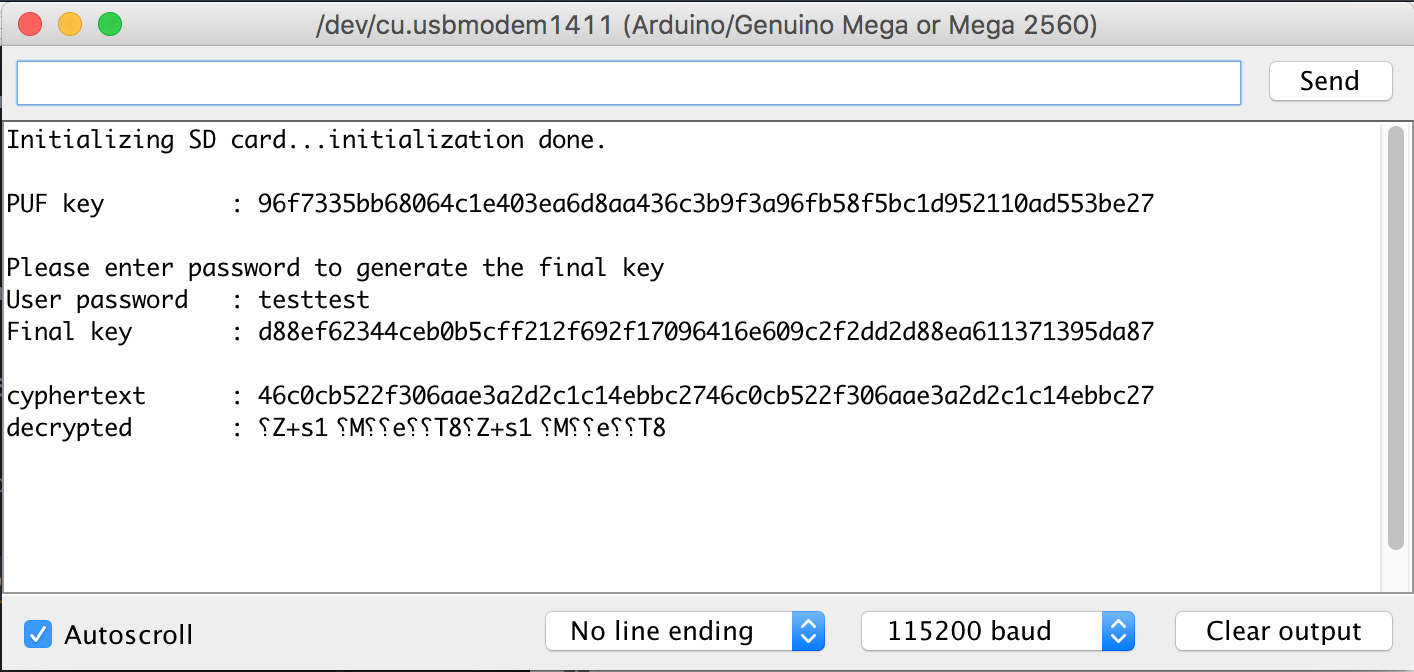
\includegraphics[width={\textwidth}]{images/C_decrypt_wrong_SRAM}}
    \caption{Screenshot of the Bitcoin key storing experiment during decryption stage. The Bitcoin key 'testpasswordtesttestpasswordtest' is previously secured by using SRAM Cypress CY62256NLL 'C' and user's password 'testtest'.
    Even though user's password is correct, the Bitcoin key cannot be reconstructed because the SRAM utilized for the decryption is SRAM Cypress CY62256NLL 'D'.}
    \label{fig:C_decrypt_wrong_SRAM}
\end{figure}

% SRAM D
\begin{figure}[tph!]
    \centerline{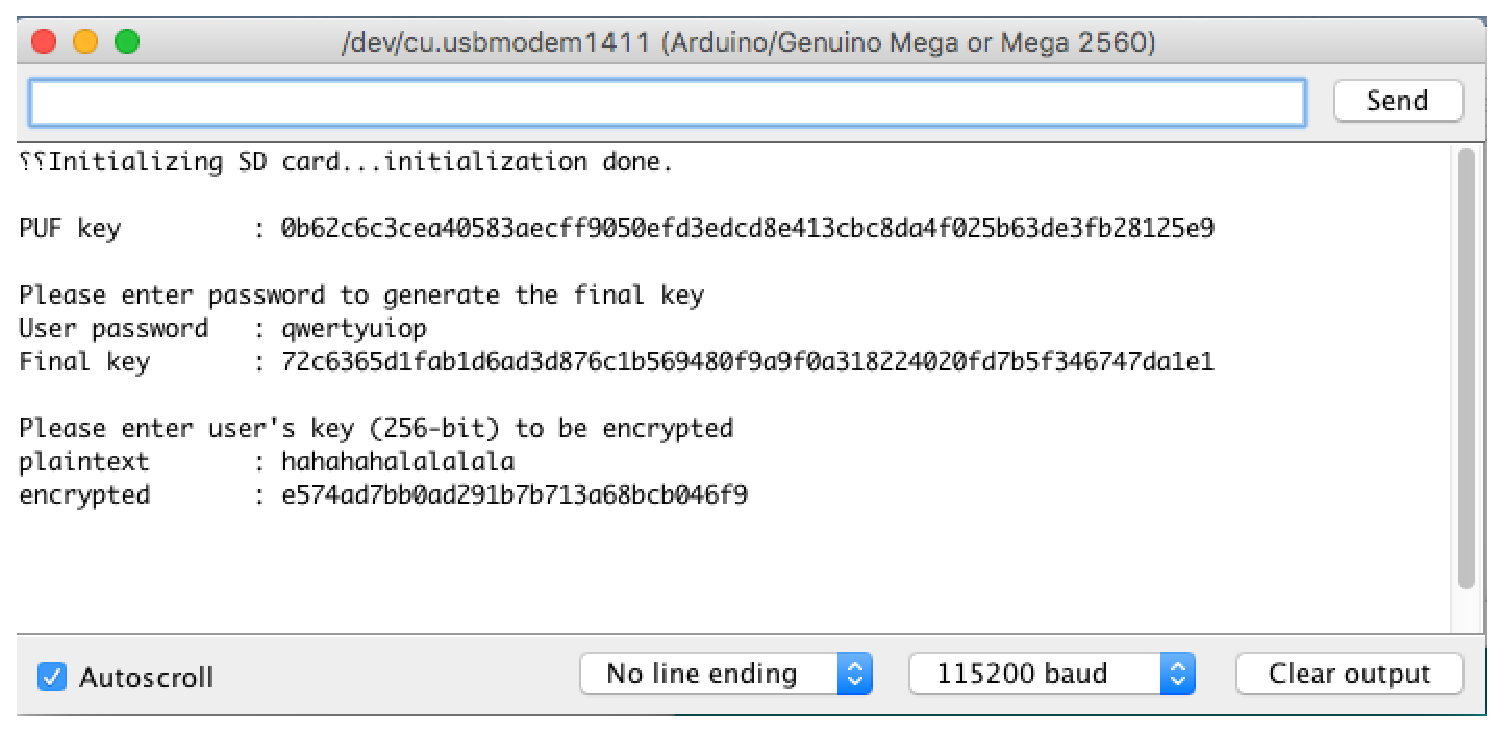
\includegraphics[width={\textwidth}]{images/D_encrypt}}
    \caption{Screenshot of the Bitcoin key storing experiment during encryption stage using SRAM Cypress CY62256NLL 'D'.
    User's password is 'passpass' and the Bitcoin key (user's key) is 'qwertyuiqwertyuiqwertyuiqwertyui'.}
    \label{fig:D_encrypt}
\end{figure}

\begin{figure}[tph!]
    \centerline{\includegraphics[width={\textwidth}]{images/D_decrypt_correct}}
    \caption{Screenshot of the Bitcoin key storing experiment during decryption stage. The Bitcoin key 'qwertyuiqwertyuiqwertyuiqwertyui' is previously secured by using SRAM Cypress CY62256NLL 'D' and user's password 'passpass'.
    The Bitcoin key can be reconstructed because user's password is correct and the utilized SRAM is SRAM Cypress CY62256NLL 'D'.}
    \label{fig:D_decrypt_correct}
\end{figure}

\begin{figure}[tph!]
    \centerline{\includegraphics[width={\textwidth}]{images/D_decrypt_wrong_password}}
    \caption{Screenshot of the Bitcoin key storing experiment during decryption stage. The Bitcoin key 'qwertyuiqwertyuiqwertyuiqwertyui' is previously secured by using SRAM Cypress CY62256NLL 'D' and user's password 'passpass'.
    Even though the utilized SRAM is the correct SRAM (SRAM Cypress CY62256NLL 'D'), the Bitcoin key cannot be reconstructed because user's password is wrong.}
    \label{fig:D_decrypt_wrong_password}
\end{figure}

\begin{figure}[tph!]
    \centerline{\includegraphics[width={\textwidth}]{images/D_decrypt_wrong_SRAM}}
    \caption{Screenshot of the Bitcoin key storing experiment during decryption stage. The Bitcoin key 'qwertyuiqwertyuiqwertyuiqwertyui' is previously secured by using SRAM Cypress CY62256NLL 'D' and user's password 'passpass'.
    Even though user's password is correct, the Bitcoin key cannot be reconstructed because the SRAM utilized for the decryption is SRAM Cypress CY62256NLL 'B'.}
    \label{fig:D_decrypt_wrong_SRAM}
\end{figure}

% SRAM E
\begin{figure}[tph!]
    \centerline{\includegraphics[width={\textwidth}]{images/E_encrypt}}
    \caption{Screenshot of the Bitcoin key storing experiment during encryption stage using SRAM Cypress CY62256NLL 'E'.
    User's password is 'qwertyuiop' and the Bitcoin key (user's key) is 'qwer1234qwer1234qwer1234qwer1234'.}
    \label{fig:E_encrypt}
\end{figure}

\begin{figure}[tph!]
    \centerline{\includegraphics[width={\textwidth}]{images/E_decrypt_correct}}
    \caption{Screenshot of the Bitcoin key storing experiment during decryption stage. The Bitcoin key 'qwer1234qwer1234qwer1234qwer1234' is previously secured by using SRAM Cypress CY62256NLL 'E' and user's password 'qwertyuiop'.
    The Bitcoin key can be reconstructed because user's password is correct and the utilized SRAM is SRAM Cypress CY62256NLL 'E'.}
    \label{fig:E_decrypt_correct}
\end{figure}

\begin{figure}[tph!]
    \centerline{\includegraphics[width={\textwidth}]{images/E_decrypt_wrong_password}}
    \caption{Screenshot of the Bitcoin key storing experiment during decryption stage. The Bitcoin 'qwer1234qwer1234qwer1234qwer1234' is previously secured by using SRAM Cypress CY62256NLL 'E' and user's password 'qwertyuiop'.
    Even though the utilized SRAM is the correct SRAM (SRAM Cypress CY62256NLL 'E'), the Bitcoin key 'testpasswordtest' cannot be reconstructed because user's password is incorrect .}
    \label{fig:E_decrypt_wrong_password}
\end{figure}

\begin{figure}[tph!]
    \centerline{\includegraphics[width={\textwidth}]{images/E_decrypt_wrong_SRAM}}
    \caption{Screenshot of the Bitcoin key storing experiment during decryption stage. The Bitcoin key 'qwer1234qwer1234qwer1234qwer1234' is previously secured by using SRAM Cypress CY62256NLL 'E' and user's password 'qwertyuiop'.
    Even though user's password is correct, the Bitcoin key cannot be reconstructed because the SRAM utilized for the decryption is SRAM Cypress CY62256NLL 'C'.}
    \label{fig:E_decrypt_wrong_SRAM}
\end{figure}


\end{document}
